%\documentclass[a4paper,twoside,12pt,dvipdfm]{report}
\documentclass[11pt, a4paper]{report}

\usepackage [shownotes]{101labs}

\addbibresource{101labs.bib}
\addbibresource{latex-exercise.bib}

\coursecode{COMP10120}
\coursename{Introductory Labs}
\title{Lab exercises}
\date{August 2013}
\author{Steve Pettifer, Toby Howard, Graham Gough and John Latham}
\bottomstuff{\noindent
\includegraphics[width=2cm]{images/rpi-logo}\hspace*{\fill}
\includegraphics[width=2cm]{images/Tux}}

\mkcmdanchor{echo}{Miscellaneous}
\mkcmdanchor{ls}{File_System_Utilities} 
\mkcmdanchor{mkdir}{File_System_Utilities} 
\mkcmdanchor{cd}{File_System_Utilities} 
\mkcmdanchor{pwd}{File_System_Utilities}  
\mkcmdanchor{rm}{File_System_Utilities}   
\mkcmdanchor{mv}{File_System_Utilities}    
\mkcmdanchor{which}{Finding_Files}    
\mkcmdanchor{gzip}{File_Compression}
\mkcmdanchor{zip}{File_Compression}
\mkcmdanchor{tar}{File_Compression}
\mkcmdanchor{man}{Getting_Help}
\mkcmdanchor{less}{File_Viewing}
\mkcmdanchor{more}{File_Viewing}
\mkcmdanchor{cat}{File_Viewing}
\mkcmdanchor{head}{File_Viewing}
\mkcmdanchor{tail}{File_Viewing}

 
  \input{includes}
  \dominitoc
  
\begin{document}

\maketitle
\tableofcontents
\clearpage


%%% Local Variables: 
%%% mode: latex
%%% End: 

\coursecode{Welcome}
\setcounter{chapter}{-1}
\renewcommand{\chaptername}{Welcome Lab Session}
\newcommand{\splunge}{\textcolor{red}{\bf SPLUNGE}}

\chapter{Getting started}
\label{cha:getting-started}

\minitoc

\section{Welcome}


Hello and welcome. In this first, introductory, lab we're going to
cover some of the basic things you'll need to know about the IT
infrastructure here in the School of Computer Science. Some of what we
tell you may well seem very obvious to you, and if that's the case
we'd ask you to be patient. Some other things might not be so obvious...

In this and every lab there will be academic staff and postgraduate students (demonstrators) around to help you. If you're stuck or find something that you really can't understand, then \emph{please ask for help}; that's what the lab staff are here for, don't just sit there getting frustrated.

All the desktop PCs in the labs in the Kilburn building are
`dual-boot': they can be started up running either Linux or
Windows. This is for flexibility -- the labs for most course units  use
Linux, but some use Windows, and of course, outside the labs, you're free to use
whichever you prefer for any aspect of your studies. If you're not
familiar with Linux, don't worry. We'll be telling you a bit about it
in this lab, and you'll be looking at it in much more detail in subsequent labs.

\section{Using Windows}
\label{sec:using-windows}

We'll start with Windows, so the first thing we need to do is to make
sure your PC is running Windows. Have a look. If it is, 
and the screen looks like Figure~\ref{figure:welc-screen}, then you  you can move on to the end of this subsection and login.

If it's currently in Linux, showing a black screen with a login prompt,  you need to reboot the PC. To do
this, press \ttout{ctrl}, \ttout{alt} and \ttout{delete}.

This will probably cause strange messages to appear on the screen,
disappear, and be replaced by yet more strange messages. Be patient,
watch it all happen, and don't worry what it all means.

After a while,
everything should settle down and the screen will look like
Figure~\ref{figure:welc-grub}.

\begin{figure}
\centerline{\includegraphics[width=15cm]{images/TH-win-welcome}}
\caption{The Windows7 Welcome screen.}
\label{figure:welc-screen}
\end{figure}

\begin{figure}
\centerline{\includegraphics[width=15cm]{images/TH-grub-win}}
\caption{The boot selection menu screen.}
\label{figure:welc-grub}
\end{figure}

This is where you decide whether to start up Windows or Linux. \emph{If you do nothing, this will automatically boot into the default operating system after a fixed timeout period. In order to stop this timeout process, just press the space bar (or any other key).}

Now use the
up/down arrow keys on the keyboard to highlight the line
reading \ttout{Windows 7}, and press the enter key. After a short while, the Windows 7
welcome screen will appear, as shown in Figure~\ref{figure:welc-screen}. Now use the ctrl-alt-del chord again as instructed and you should see the Windows 7 login screen, as shown in Figure~\ref{figure:login-screen}.

\begin{figure}
\centerline{\includegraphics[width=15cm]{images/TH-win-login}}
\caption{The Windows 7 login screen.}
\label{figure:login-screen}
\end{figure}

To log in to your personal account, type in your username (this is an
8-character name starting with an `m' that you were given at registration). Your password will
be the one  you set at registration. If your password doesn't work, or if you've forgotten it,
you need to fix this urgently. You can:

\begin{itemize}
  \item On a machine running Windows, login with the username \ttout{register} and password \ttout{register}, then follow the instructions.
\item If you have access to a web browser, use the password recovery page at\\ \url{https://iam.manchester.ac.uk/recovery_login/overview}
%\item Visit the \verb|it.changes| Helpdesk in Kilburn Lower First area (Welcome Week, 09:00 -- 17:00)
\item Outside lab times, you can contact the University IT helpdesk (opening hours are Monday to Friday 9am to 5pm.) by phone on 0161 306 5544, or dial 65544 from a University internal phone; or you can visit the helpdesk in John Rylands Library (Building 55 on
the Campus Map), at the top of the escalator in the Blue 1 area.
\item Remember, if you need help, ask!
\end{itemize}

Once you're logged in, go to your MyManchester page in a web browser, at

\url{https://my.manchester.ac.uk}

This page should look something like Figure~\ref{figure:welc-mymanchester}.

\subsection{Reading your email}

We use email extensively in the School, so it's vitally important that
you read your mail regularly -- at least once a day (and probably much
more often!). Follow the mail link (indicated by the green arrow in
Figure~\ref{figure:welc-mymanchester}) to access your email on the
University's Office365 system. This is a fully-featured system that
gives you 25GB of email storage space and an integrated calendar. You should
see a page looking something like Figure~\ref{figure:welc-mail365}.

Have a look around for a few minutes and check what mail you've
got. In particular, look for one with ``The Monday Mail'' in the
Subject line. This an important mail you'll receive every Monday
(hence the name) throughout your 3 or 4 years with us in the
School. The Monday Mail tells you what's going on each week in the
School. Take a moment to read it now. You can always read the Monday Mail, by the way, at the archive located at\\  \urlnop{studentnet.cs.manchester.ac.uk/ugt/mondaymail/}

\begin{figure}
\centerline{\includegraphics[width=15cm]{images/hamza-email-link.png}}
\caption{Your MyManchester page.}
\label{figure:welc-mymanchester}
\end{figure}

\begin{figure}
\centerline{\includegraphics[width=15cm]{images/hamza-365-mail.png}}
\caption{Your Office365 email.}
\label{figure:welc-mail365}
\end{figure}

\label{sec:reading-your-mail}

Office365, like most modern email systems, supports the IMAP
protocol -- which means that you can access your mail from any device
that can run an IMAP mail client. Some examples of such clients are:
Mozilla Thunderbird, Mac Mail, Windows Live Mail and mail apps on mobile devices. No matter what
client you use, you need to tell it the appropriate settings. The mechanism for finding these setting can be found in our student wiki, which is located on the web at \urlnop{wiki.manchester.ac.uk/compsci/index.php/It.changes}. Look for the answer to question 'How do I configure my favourite IMAP mail client?'. This wiki provides help about the major changes we have made to our IT infrastructure this summer; there is also a general FAQ at \urlnop{wiki.manchester.ac.uk/compsci/index.php/StudentFAQ}. Please make use of these useful sources of information.

Once you've found the settings, use Office365 to email this information to yourself, to your
University account:

\url{firstname.lastname@student.manchester.ac.uk}

You'll need this information in a later lab so please don't delete this email after you've read it.

Finally, if you use an IMAP mail client on your phone or mobile
device, configure it to use the settings you've just found, and check
that you can read and send email successfully.

That's all on Windows for now, but of course  you're free to boot an available PC into Windows  and use it at any time unless you are in a lab that requires the use of Linux. Next, we're going to take a first look at Linux.

\subsection{Rebooting into Linux}
\label{sec:rebooting-into-linux}

So let's reboot the PC, and start it up in Linux. First, log out of
Windows by selecting the Windows icon in bottom left and then \ttout{Log off}). Get back to the login screen, click the
small icon in the lower right of the screen (see Figure~\ref{figure:welc-restart}) and select \ttout{Restart}.

\begin{figure}
\centerline{\includegraphics[width=0.4\textwidth]{images/TH-shutdown-win}}
\caption{Restarting the PC.}
\label{figure:welc-restart}
\end{figure}

The system will shut down and we'll be back to the boot selection menu
screen we saw earlier in Figure~\ref{figure:welc-grub}. This time, use
the up/down arrow keys to select \ttout{EPS Linux (Scientific
  Linux)}. Linux will now start, and after a short while you should
see a black screen, with a white login prompt. We won't login to Linux
at this stage, that can wait until a later lab, next week. We would,
however, like you to read the rest of this document, which gives you
some useful and interesting background information about Linux. If you
don't have time to finish reading it in the lab, please make sure you
do so before the next lab session.

%\section{Using the School Linux system}
\section{Unix and Linux}

Over the next couple of weeks you will be undertaking a number of
introductory labs to familiarise yourself with the School's computing
infrastructure. Much of this is based on devices and machines running Linux, a
variant of the Unix family of operating systems; this document
provides some background on Unix and explains why we think it is
important. It would very useful if you could read this before you
attend the first introductory labs, where the emphasis will be on
leading you through a series of tasks to explore our setup.

\subsection{Operating Systems}

An \wikipedia{Operating_system}{operating system} (OS) is a suite of
software that makes computer hardware usable; it makes the `raw
computing power' of the hardware available to the user. You're
probably most familiar with
the \wikipedia{Microsoft_windows}{Microsoft Windows} and
Apple \wikipedia{OS_X}{OS X} families of operating systems for
`desktop' computers, and \wikipedia{Ios}{iOS} (Apple, again) and
Google's \wikipedia{Android_(operating_system)}{Android} for mobile
devices; but many other more specialist operating systems exist, and
you'll be studying some of these and the principles that underpin OS
design in COMP25111 in your second year. In the meantime, a potted
history of OS development will tide us over\ldots
 
\subsection{Unix Origins}
\label{sec:unix}

In the late 1950s, an American company
called \wikipedia{Bell_Labs}{Bell Laboratories} decided that they
needed a system to improve the way they worked with their computer
hardware (it's probably quite hard to imagine what interacting with a
computer \emph{without} an operating system might be; but it wasn't
pretty and involved manually loading and running programs one by
one). Together with the \wikipedia{General_Electric_Company}{General
Electric Company} and the \wikipedia{MIT}{Massachusetts Institute of
Technology}, they set about the design of an operating system they
called \wikipedia{Multics}{Multics}: the `Multiplexed Information and
Computing Service'. Multics was hugely innovative, and introduced many
concepts that we now take for granted in modern operating systems such
as the ability for more than one program to run `at once'; but it did
rather suffer from `design by committee', and the final system was
seen at the time as being overly complex and rather bloated (`bloated'
is all a matter of perspective of course: its sobering to realise
though that the entire Multics operating system was only around
135Kb. Today's operating systems are something like 30,000 times this
size\ldots). In the late 1960s, a group of programmers at Bell Labs
created a cut-down, leaner and cleaner version of Multics that would
work on more modest hardware. Legend has it that this was to allow
them to play their favourite (only!) computer
game, \wikipedia{Space_Travel_(video_game)}{Space Travel}. In an early
example of the trend of giving things `punny' names, to contrast with
the more clumsy Multics, they called this new system Unix. The
so-called \wikipedia{Jargon_File}{Jargon File} is a good source of
explanations of various bits of computer slang and their obscure
origins, and is well worth a read: in part to give some background
history, but mostly as an insight into the minds of the computing
pioneers of the past!

%\begin{htmlonly}
%(See the Unix entry in the useful and amusing
%\htmladdnormallink{Jargon
%file}{http://www.new.ox.ac.uk/admin/jargon/html/entry/Unix.html}, a
%file}{http://www.cs.manchester.ac.uk/software/jargon/html/entry/Unix.html}, a
%file}{\jargonFileUnix}, a
%`collection of slang terms used by various subcultures of computer
%\htmladdnormallink{hackers}
%{http://www.cs.manchester.ac.uk/software/jargon/html/entry/hacker.html}'.)
%{\jargonFileHackers}'.)
%\end{htmlonly}

Even though Unix is now quite old, most Computer Scientists recognise that the designers of Unix got most of the fundamental concepts and
architecture right. Given how much computing has changed since the 1960s, this was an astonishing intellectual achievement. Although Microsoft's \wikipedia{Microsoft_Windows}{Windows} is by far the most common operating system on \emph{desktop} machines, the majority of the Internet, much of the world's corporate infrastructure, virtually all supercomputers, and even some mobile devices are powered by Unix-like operating systems. So, while the polished graphical user interfaces of Windows and \wikipedia{OS_X}{OS X} appear to dominate the world of computing, most of the real hard-core and leading-edge computation relies on an elegant operating system designed nearly 50 years ago (by a team of scientists who wanted to play a game).  

\subsection{Modern Unix Variants}
\label{sec:modern-unix-variants}


The history of Unix is complex and convoluted, with the system being updated, re-implemented, and mimicked repeatedly over the years, primarily by commercial companies who guarded their versions jealously. Figure \ref{fig:unix-history} shows a tiny fragment of the Unix's `family tree' (the full diagram, which you can find at \urlnop{www.levenez.com/unix/unix.pdf}, is \emph{many} times the size of the portion you can see here).

\begin{figure}[h!tb]
  \begin{center}
    \includegraphics[width=13cm]{images/unix}
  \end{center}
\caption{A fragment of \'{E}ric L\'{e}v\'{e}nez's Unix History chart, reproduced with permission and showing the beginnings of Linux in amongst other versions of Unix.}
\label{fig:unix-history}
\end{figure}
 
Although many of the branches represent interesting innovations of one kind or another, there are perhaps two that deserve particular attention. The first of these was the decision by Apple some time around the turn of the millennium to drop their own---highly popular, but ageing---bespoke operating system (unimaginatively called \wikipedia{Mac_os_9}{Mac OS 9}) in favour of a Unix-based system (now the more familiar `OS X', where `X' is both the Roman numeral `10' and a nod in the direction of the uniX nature of the OS). Although the majority of Mac users are blissfully unaware of the fact, behind the slick front-end of OS X, sits a variant of Unix. The second, and perhaps more profound of these events was the creation in 1991 by Swedish programmer \wikipedia{Linus_torvalds}{Linus Torvalds} of a Unix-like system, the source code to which \emph{he gave away for free}\footnote{`free' here in the sense both of `freedom to reuse or adapt', and also in the sense of `without charge'.}; this became known as the \wikipedia{Linux_kernel}{Linux Kernel}. Combined with other free software created by the \wikipedia{Free_software_foundation}{Free Software Foundation}, a non-commercial version of Unix called \wikipedia{GNU/Linux}{GNU/Linux} was born (GNU here is a recursive acronym for ``GNU's not Unix'', a swipe at other commercial non-Free versions; much to the annoyance of the Free Software Foundation, GNU/Linux is almost always called just `Linux'\footnote{Linux
is pronounced ``Linn-ucks'', despite the fact the name was coined by
its creator, and his name `Linus' is pronounced
``Leen-uss''!}.) 

Linux has been, and continues to be, developed cooperatively by
thousands of programmers across the world contributing their effort
largely free of charge. It is amazing to think that such
a project could ever happen---and it is surely a testament to the
better side of Human nature. But what is interesting is the
observation that these programmers are not motivated by commercial
concerns, but by the desire to make good reliable software and have it
used by lots of people. Thus, Linux is a good choice of Unix: it's
Free, it's efficient, and it's reliable, and it is now used by large corporations, governments, research labs and individuals around the world. Even Google's \wikipedia{Android_(operating_system)}{Android} platform is a Linux-based mobile OS, and the  \wikipedia{Amazon_Kindle}{Amazon Kindle} is also a Linux box behind the electronic ink of its user interface (Figure \ref{fig:kindlelinux}).

\begin{figure}[h!tb]
  \begin{center}
    \includegraphics[width=13cm]{images/kindleroot}
  \end{center}
\caption{A photograph of Liraz Siri's `rooted' kindle, showing the Linux command prompt. Reproduced with the author's kind permission from \urlnop{www.turnkeylinux.org/blog/kindle-root}}
\label{fig:kindlelinux}
\end{figure}

One of the results of the fact that Linux is Free is that several
organisations and companies have created their own distributions of
it; these vary a bit (in fact, anybody is free to make any change they
like to Linux, and pass it on to whoever wants it). The distribution
we use in this School is \textbf{Fedora}, which is
one of the most popular and is sponsored by a
US company called \textbf{Red Hat}.
%, which is the latest release

So, if you are to become an expert computer professional, it is
important that you understand the theory and practice of Unix based
systems. Learning Unix is not only a crucial skill for any serious
computer scientist, it is a very rewarding experience; the labs over
the next couple of weeks are designed to help you become familiar with what will be your daily working environment.


\renewcommand{\chaptername}{Intro Lab Session}
\coursecode{Introductory Labs}
\chapter{Getting started with Raspberry Pi}

\notesurl{rpi1}

% TODO: Intro to what they have been given, and labelling their Pi
% TODO: References, references.
% TODO: Wikipedia links
% TODO: The Pi is yours to keep; if you lose it you'll have to buy another
% TODO: What you'll need to use the Pi at home
% TODO: Where do we introduce 'devices', 'files' and 'processes'? They will see virtual devices like tty0 and sda1 

The Raspberry Pi is an astonishing piece of hardware. Not because it is super-fast or super-powerful---it's actually quite a slow computer by today's standards---but because it is small, cheap and needs very little energy to run. Its cheapness means you can experiment with it safe in the knowledge that if you mess it up, lose it, or drop it into the canal, getting hold of a replacement isn't going to cost you much more than a text-book or a night out at the cinema. Its small size and fairly modest power requirements mean you can be put to use in lots of applications where a regular-sized PC would be impractical.  We hope this will encourage you to experiment and explore, and to take risks playing with both its hardware and software that you might be reluctant to do on your own computer or tablet, or simply can't do with the School's lab machines. 

This lab session is designed to get you familiar with the Raspberry Pi itself, and with some of the basics of the Linux operating system it uses. We're going to be covering a lot of ground quite quickly, and it's important that you read these notes carefully and follow the instructions precisely for now. As the lab sessions progress, the instructions will become much less prescriptive, and we'll be encouraging you to experiment and explore much more, and to find out things for yourself. But for now, just follow our lead. 

Scattered throughout the main text of these exercises there are information boxes of various kinds:
\\

\begin{tabular}{m{1.5cm}m{12cm}}
{\includegraphics[width=1.5cm]{images/bomb}} & \textbf{Danger!} The bomb icon explains problems and pitfalls, and how to avoid them. It's really important that you read these sections, or you may regret it later.\\
\\

\includegraphics[width=1.5cm]{images/rpi-logo} & \textbf{Raspberry Pi Facts and Factoids.} These sections explain useful but non-essential things about the Raspberry Pi. If you're pushed for time, you can safely skip these boxes and perhaps come back to them another time.\\
\\
\includegraphics[width=1.5cm]{images/diversion} & \textbf{We digress\ldots} Boxes marked with this icon contain digressions and facts that are hopefully interesting but are probably tangential to the main flow of the exercise.\\
\end{tabular}

\FloatBarrier 
\section{The Raspberry Pi}

The most remarkable thing about the Pi is that, although it's a bit underpowered in many ways, it is capable of running the same full Linux Operating System as the machines that you'll be using in the labs for the duration of your studies, and which you'll undoubtedly encounter in your future careers. Actually we're going to be using slightly different flavours of Linux on the Pi and the lab machines, but the differences are fairly minor---more on that later. Let's get started. 

The Raspberry Pi itself is just the circuit board shown from the top in Figure \ref{figure:bare-rpi}. The case we've put yours in is clear plastic so you can see the Pi inside, but you're welcome to change it for another style if you prefer (there are plenty available to buy online, and lots of people have made their own unique ones just for the fun of it). The Pi is reasonably robust, and you can use it without a case, but obviously it's a bit more vulnerable if its not in a box of some sort. Figure \ref{figure:bare-rpi-underside} shows the Pi's circuit board from beneath, with an SD card inserted.

\begin{rpi}{Why Pi?}
  The Raspberry Pi apparently got its name because (a) lots of other computer systems have been named after fruit (you'll know of Apple and Blackberry, but in the past there has also been at least Apricot and Tangerine), and (b) the \wikipedia{Python_(programming_language)}{Python language} was one of the first things ported to run on it. The logo was created by Paul Beech, and is based on Buckminsterfullerene, a spherical fullerene molecule more commonly called a Buckyball. Its designer pointed out that a full buckyball has 32 faces, but that only 11 are visible in the 2D logo; and that the Raspberry Pi has a 32-bit processor and an ARM11 on board.

The ARM processor, on which the Pi and the vast majority of the world's other mobile devices are based, was originally designed by a team led by \wikipedia{Steve_Furber}{Steve Furber}, who is a Professor in this School.  
\end{rpi}

\begin{figure}
\centerline{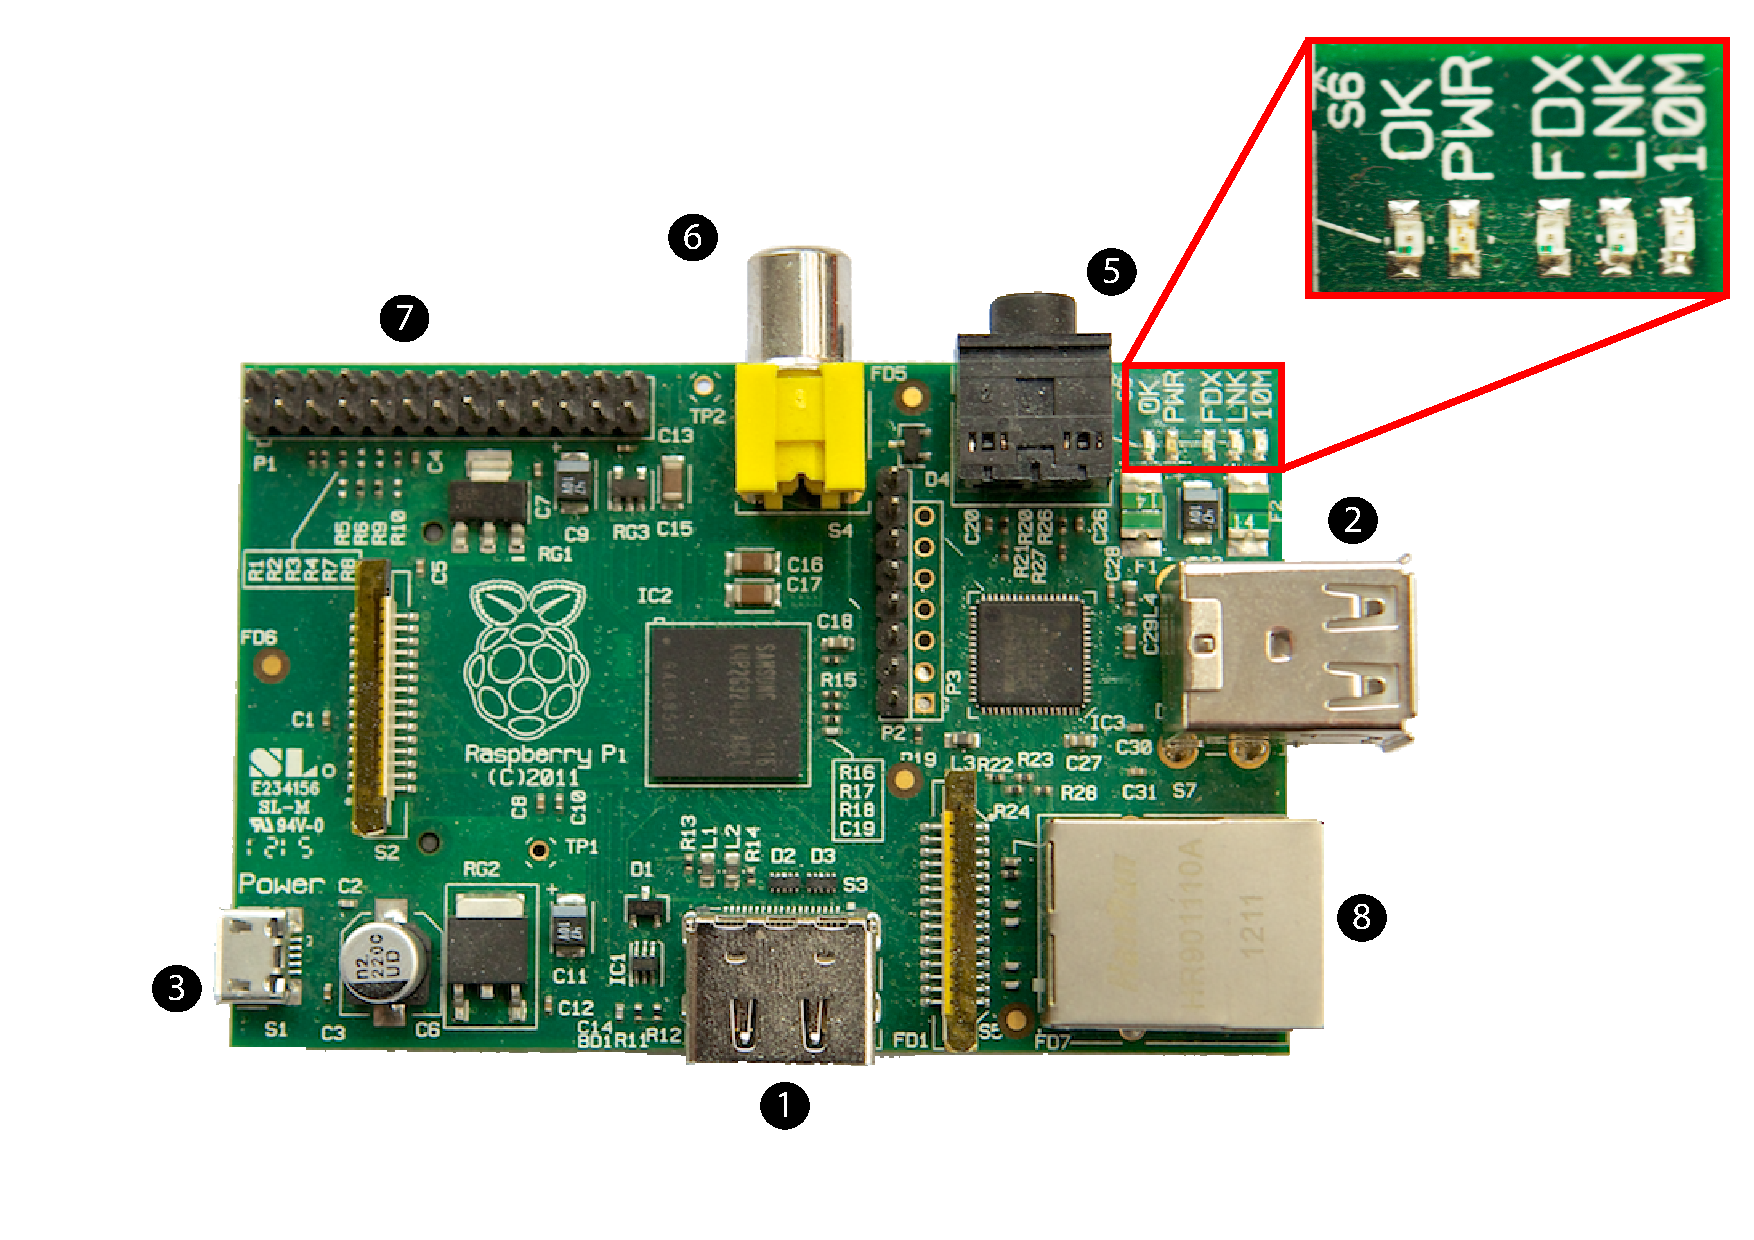
\includegraphics[width=15cm]{images/bare-rpi-annotated}}
\caption{An uncased Raspberry Pi, and an expanded view of the indicator LEDs at the board's top right. The numbered connectors are \protect\circled{1} HDMI output,  \protect\circled{2} USB,  \protect\circled{3} power,  \protect\circled{5} audio output,  \protect\circled{6} composite video out,  \protect\circled{7} General Purpose Input/Output (GPIO),  \protect\circled{8} Ethernet.}\label{figure:bare-rpi}
\end{figure}

\begin{figure}
\centerline{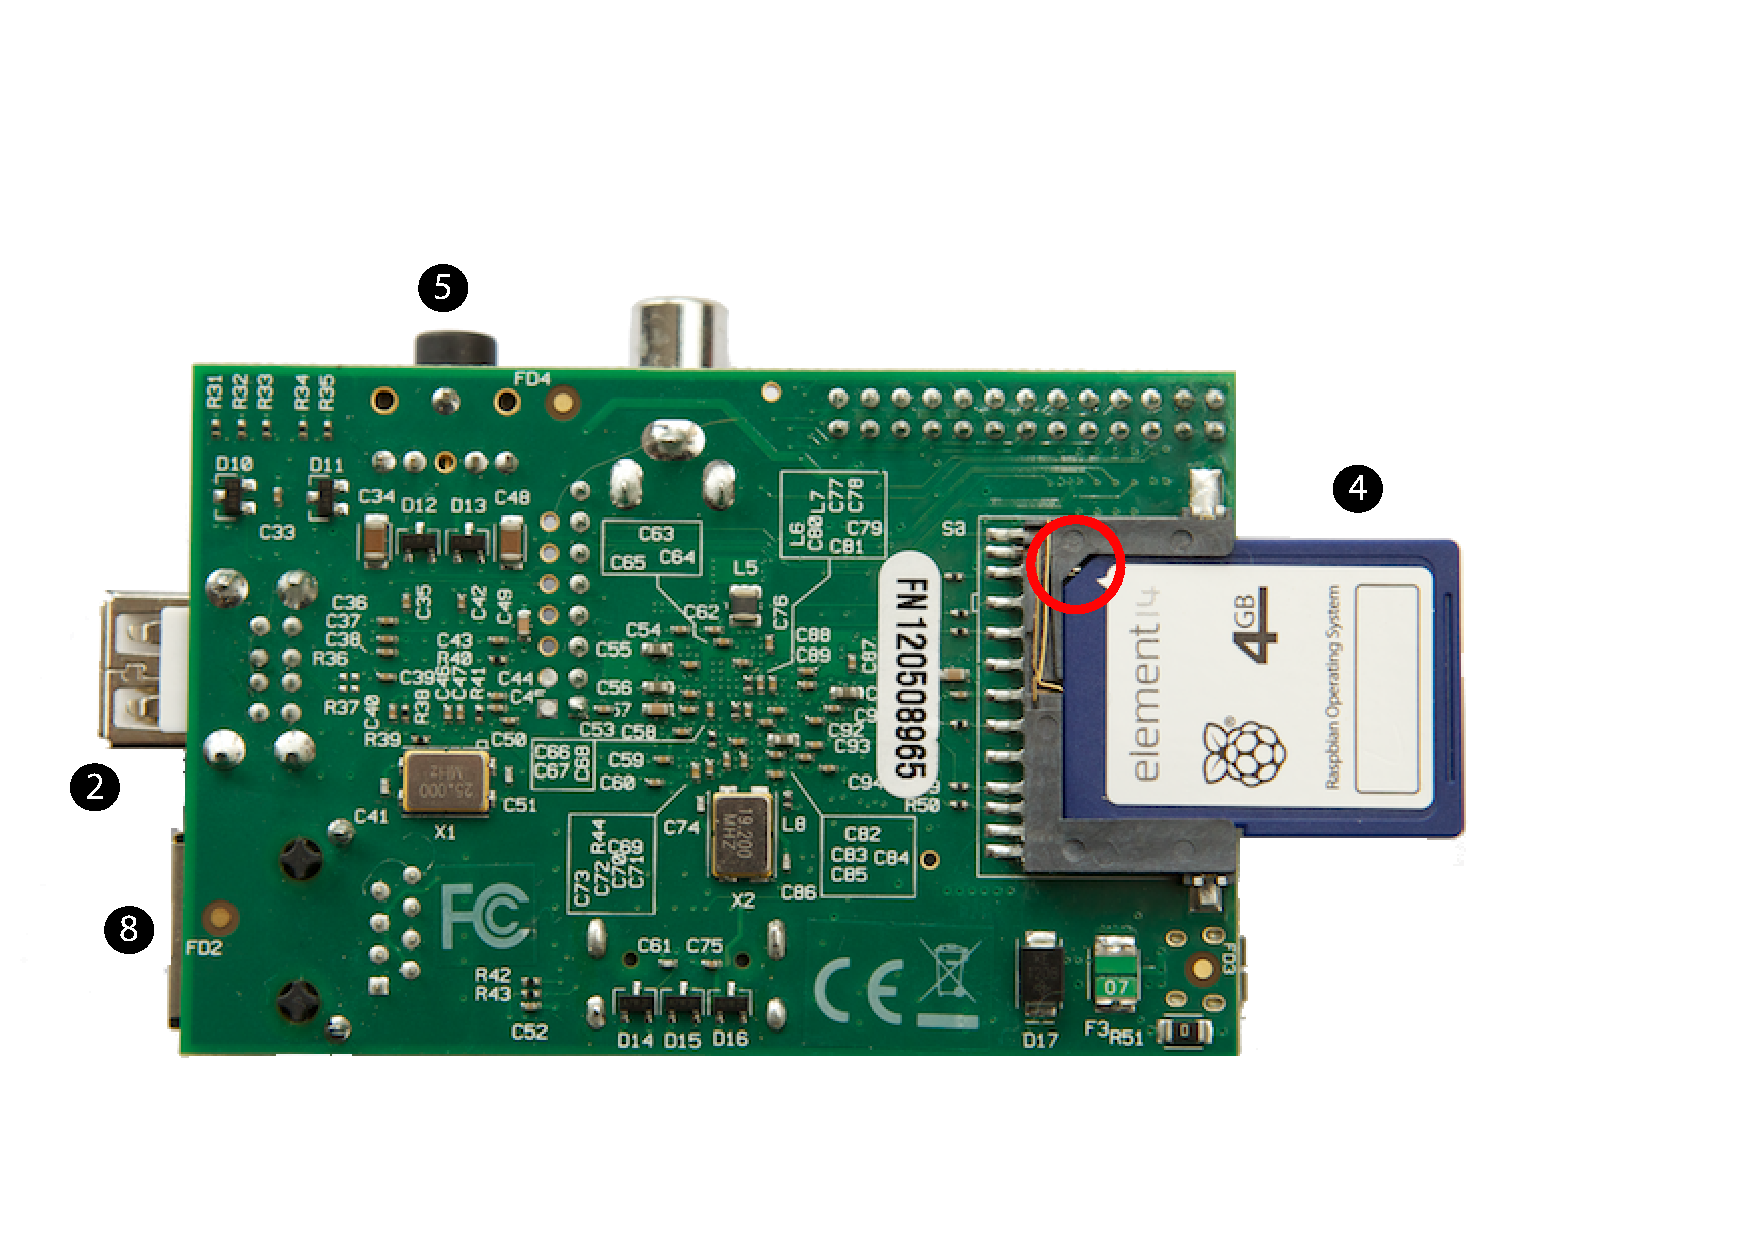
\includegraphics[width=15cm]{images/bare-rpi-underside-annotated}}
\caption{A naked Raspberry Pi. The circle indicates the location of the bevelled corner to orient the card. The ports are numbered as in Figure~\ref{figure:bare-rpi}, and in addition \protect\circled{4} shows the location of the SD (Secure Digital) memory card. The red circle indicates the locating bevel on the card.}\label{figure:bare-rpi-underside}
\end{figure}

It's important that you connect the Pi up in exactly the order specified here---so even if you are familiar with using a Pi, please don't jump ahead and plug everything in at once (no harm will come to the Pi if you do, but this exercise relies on your following our instructions closely). The monitors in the LF31 Lab are all fitted with an extra video lead for connecting up the Pis. Locate the HDMI lead, and plug this into the socket marked \circled{1} on Figure~\ref{figure:bare-rpi}. Next we'll need to connect a keyboard. Follow the cable that comes out the back of the keyboard towards where it vanishes into the desk, and you'll see an inline USB connector that will allow you to unplug the keyboard from the desktop PC and into one of the two USB sockets on your Pi; these are marked with \circled{2} on the Figure. It doesn't matter which USB socket you choose, but please make sure to reconnect this to the PC when you're done with these experiments, just as a courtesy to the next user. 

Next, we need to insert the \wikipedia{Secure_Digital}{Secure Digital} (SD) card that contains the Pi's operating system, and on which you'll be storing your own files. Look at Figure ~\ref{figure:bare-rpi-underside}, make sure the SD card is orientated correctly (note the position of the little cut corner) and gently push it into the socket; around half of the card will remain protruding outside the case. \textbf{Don't} plug a mouse in at this stage; you won't need it until the very last part of the exercise.

\begin{rpi}{Raspbian}
  The SD card we've provided for you has already had the standard Raspbian version of Linux written onto it (it's a version of the Debian release of Linux, tuned for the Pi). If you do manage to corrupt the operating system, or just want to start from scratch, then re-writing the SD card with a fresh image is reasonably straightforward: there are plenty of instructions online on how to do this, and we've provided you with a USB multi-card reader/writer that you can use for the job. The process does require access to what's called the `raw' device though, and on Linux that requires administrator access to the machine, so you'll have to use your home machine or someone else's Raspberry Pi to do this.

  Instructions on how to get hold of the files you'll need, and how to write them to the SD card on various operating systems are available at \urlnop{www.raspberrypi.org/downloads}. You might want to think about getting a larger SD card in any case; the one we've given you is fine for the labwork we've set, but probably a bit on the small side for anything else. SD cards are widely available in shops and online, and aren't expensive. But you should check whether the specific card you're going to buy is compatible with the Pi before parting with any money---differences in the read/write speeds of some cards mean they don't play nicely with the Pi.
\end{rpi}

Now you're ready to power up the Pi. From the back of the monitor you'll notice a Micro USB cable (the same connector that you'll find on many modern smartphones and tablet devices). This goes into the socket marked \circled{3} on Figure \ref{figure:bare-rpi}. There is no power switch on the Pi, so as soon as the power cable goes in, it will start to boot (this strange term is explained in breakout box~\ref{boot box}): the red PWR LED should light up and stay on, and you'll also notice that the OK LED (which indicates SD-card activity) to its left also flickers. If any of the other three LEDs marked FDX, LNK, or 10M are lit, then that means you've already plugged a network cable into your Pi, in which case please unplug that now!

\begin{danger}{Pi Power} 
Like most other computers, the Pi doesn't like having its power removed without being shut down properly. Although you might get away with it, there's a reasonable chance of messing up the operating system if you remove the power while the Pi is in the middle of doing something. And because the Pi runs a multi-tasking operating system, it's almost always `doing something', so pulling the power out unexpectedly is always a bad idea. You're unlikely to damage the Pi's hardware like this, but you may find that you lose work, and may have to reinstall the operating system. For instructions on how to shut the Pi down safely, see Section \ref{section:shutdown}.
\end{danger}

Refer to Figure~\ref{figure:monitorswitch} and switch the Input Selection on the monitor from VGA (which is the input used by the PC under the desk) to DVI (the cable you've connected your Pi to is a HDMI to DVI cable), and all being well you should see a black screen containing the Raspberry Pi logo at the top left, and white text that scrolls up the screen as the Pi boots. When the boot process finishes for the first time (it will take somewhere about 20--30 seconds), if all has gone well you should see the Pi's configuration tool appear (see Figure \ref{figure:raspi-config}).

% TODO: needs a photo of the monitor / switch here
\begin{figure}
\centerline{\includegraphics[width=5cm]{images/mysteryimage}}
\caption{The Input Selection switch on the monitor.}\label{figure:monitorswitch}
\end{figure}

\begin{diversion}{Booting}
\label{bootbox}
The phrase `booting' to refer to the process of starting up some computer system has become quite commonplace, but its origins are rather strange. It's thought to have first been used in early 19th Century America as a way of describing an obviously impossible action such as to ``pull onself over a fence by one's bootstraps''. These days it is used to refer to any self-sustaining process that is able to happen without external help. 

So why is starting a computer a bootstrapping process? In order for you as a user to be able to run a program, the computer needs an operating system. But in order to load its operating system, it needs some instructions that tell it how to understand the file system. And in order to load the instructions that tell it how to understand the file system it needs to\ldots well, you get the idea. In reality, most computers have a very small set of instructions hardwired into them that begin the process of loading a  slightly more complex `bootloader', which then begins the process of loading the OS kernel and any modules needed to interact with the hardware, and then starts loading services and features of increasing sophistication that rely on the simpler ones loaded previously to function. 

As an aside, you want to consider this: if you need a text editor to write programs, how did the first text editor (which is itself a program) get written?
\end{diversion}

\begin{figure}
\centerline{\includegraphics[width=13cm]{images/raspi-config.png}}
\caption{The Raspberry Pi config tool. The highlight bar can be moved between the different controls using the Tab key, or up and down in the menu using cursor keys.}\label{figure:raspi-config}
\end{figure}

Before using the Pi for real, you'll need to perform one task using this menu. Use the up and down cursor keys to move the selection bar to the \ttout{expand\_rootfs} option, and press Enter. You'll see a confirmation that `Root partition has been resized. The filesystem will be enlarged upon the next reboot'. If that doesn't mean anything much to you right now, don't worry, we'll come back to an explanation of that later (see Section~\ref{section:expandfs}). For now just press Enter again to get back to the main menu. 

At this stage you could tweak various other options that affect the display and the layout of keyboard being used; but conveniently the defaults set on the Pi will do just fine for now (it is a mostly British invention after all, so it defaults to UK keyboard layout!) Use the Tab key to move the red highlight to \ttout{<Finish>}, and hit Enter again. The Pi will reboot (an example of what this looks like is shown in Figure \ref{figure:piboot}) and this time when the process finishes you'll be presented by a UNIX login prompt which will say something like:

\begin{figure}
\centerline{\includegraphics[width=15cm]{images/bootscreen}}
\caption{A sample Raspberry Pi bootscreen. The exact layout and details may vary depending on the size/shape of the screen and the configuration of the Pi.}\label{figure:piboot}
\end{figure}

\begin{ttoutenv}
Debian GNU/Linux wheezy/sid raspberrypi tty1

raspberrypi login:
\end{ttoutenv}

At the login line enter \totype{pi} as the username, and when prompted for the password, type \totype{raspberry}. \textbf{Note that the username will appear on screen as you type it, but the password will not} (so make sure you're typing carefully!) You should see:

\lstset{moredelim=[is][\textbf]{|}{|}}
\begin{lstlisting}
Last login: Sat May 11 14:20:48 BST 2013 on tty1                                                                                                   Linux raspberrypi 3.2.27+ #250 PREEMPT Thu Oct 18 19:03:02 BST 2012 armv6l

The programs included with the Debian GNU/Linux system are free software;
the exact distribution terms for each program are described in the
individual files in /usr/share/doc/*/copyright.

Debian GNU/Linux comes with ABSOLUTELY NO WARRANTY, to the extent
permitted by applicable law.
|pi@raspberrypi ~ $|
\end{lstlisting}


%

The last line of this text (which is shown in bold here but will be green and blue on your screen) is the command prompt. It might look innocent enough, but in the right hands, the command prompt is one of the most powerful ways of controlling a computer. It may feel a bit odd at first if you're used to a graphical interface, but being comfortable with issuing instructions to a machine via a textual command-line rather is a crucial skill that you'll need during your studies here at University, and also in your future career. In fact, employers have often said that our students' abilities with the command line come as a very pleasant surprise to them.


\begin{diversion}{Don't be a WIMP}
The familiar Windows, Icons, Menus and Pointer (WIMP) paradigm used on most graphical desktop environments is enormously powerful, but it's not suitable for every task, and understanding when you're better off using the command-line or a keyboard shortcut instead will make you a lot more efficient.

Sometimes the clumisness of the GUI comes from the fact that there's no convenient visual metaphor for a particular action; how do you graphically represent the concept of `rename all the files I created yesterday so they start with a capital letter'? 

But a lot of the time the issue is simply that it takes much longer to do some things with the mouse than it does with a keystroke or two. Every time you use the mouse, a little time is wasted shifting your hand off the keyboard and a little more time used up tracking the pointer between the on-screen widgets. For casual use, this wasted time really doesn't matter. But as a computer scientist you're going to be spending a lot of time time in front of a machine, and all the seconds wasted moving the mouse pointer around add up. 

What's really fascinating here, though, is that although the keyboard versus mouse debate is one that has been running for at least the mid-1980s, there isn't a clear winner, or even any definitive guidelines as to when one is better than the other. 

In any case, you should definitely learn the keyboard shortcuts for the most common operations in your favourite tools, and a handful of useful command-line tools. For example, when you're writing code you'll be saving files very regularly; maybe even several times a minute when you're debugging. There are two options for this: 1) move hand off keyboard to mouse; use pointer to find the `File' menu, from the file menu move the pointer to the `Save' option; move hand from mouse back to keyboard. Or 2) Press the combination of keys that perform the `save' function. Which do you think is faster?

And think carefully about the best tool for the job; sometimes it'll be the mouse/menu combination, but perhaps more often than you might think, a few selected commands may get the job done considerably more quickly. In particular, you've probably had more experience of doing things the GUI-way up until now, so if it's not obvious which is the better choice for a particular task, we suggest you go for the command-line option until you're familiar enough with the pros and cons of both approaches to make an informed decision each time.
\end{diversion}

The default command prompt on the Pi consists of four components shown in Figure \ref{figure:prompt}.

\begin{figure}
\centerline{\includegraphics[width=7cm]{images/default-prompt}}
\caption{The different components of the Pi's default command prompt.}\label{figure:prompt}
\end{figure}


\begin{itemize}
\item To the left of the \ttout{@} symbol is the name of the user, and in this case that's \ttout{pi}, since you've just logged in under that name
\item To the right of the \ttout{@} is the hostname of the machine, which on a Raspberry Pi is quite reasonably set to \ttout{raspberrypi} by default.
\item The \texttildelow{} tells you where in the filestore you're currently working. We'll explain this in a lot more detail later on, for now all you need to know is that the \texttildelow{} symbol is called a \textit{tilde} (pronounced something like till-duh, though locally its often referred to colloquially just as a `twiddle'), and is used here to refer to the `home' of the current user. 
\item the \$ symbol signifies that you can type your commands from here on. 
\end{itemize}

You can change this prompt to something more or less verbose later, but for now we'll leave it as it is. For simplicity in these notes, we'll use the \$ notation from now on to mean `type something at the command prompt and press Enter'. So for example

\begin{ttoutenv}
$ echo Hello World
\end{ttoutenv}

\noindent means `type \totype{echo Hello World} at the command prompt and then press Enter' (you can do this if you like; the result will be that `Hello World' gets `echoed' back to you on the next line of the screen). 

Before we do any real work on the Pi, we should make it a bit more secure than it currently is. Remember, you've logged in using the default username `pi' and the default password `raspberry', so anybody else could do the same. To change the password to something that's unique. For inspiration and advice on creating good passwords, see Figure \ref{figure:xkcd-password}.

\begin{figure}
\centerline{\includegraphics[width=13.5cm]{images/xkcd-password-strength}}
\caption{XKCD's take on password creation \urlnop{xkcd.com/936/}}\label{figure:xkcd-password}
\end{figure}

The command to change the password is \totype{passwd}; typing this at the command prompt and entering your current (i.e. `raspberry') and new password (twice, to be sure), should look like this:

\begin{ttoutenv}
$ passwd
Changing password for pi.
(current) UNIX password:
Enter new UNIX password:
Retype new UNIX password:
\end{ttoutenv}

\noindent Note in the above, we're using lines that don't start with the dollar symbol to show output as a result of what you've typed, and that none of the passwords you're typing actually appear on screen for obvious sneaky over-the-shoulder-peeking reasons. \textbf{Don't forget this password: there's no easy way to get back into your Pi without resetting everything.}

\begin{danger}{Memory Loss} 
Although the Pi uses a fairly standard UNIX operating system, it's probably not quite as secure as a normal desktop machine because of its small size and easily-removable storage media. Once the Pi has booted from the SD card, it's about as secure as any other Linux machine. But because the memory card is easily removable, it can trivially be connected to another machine as a `removable media' device; and at that point the host machine can almost certainly see its contents, including any of the files you've created, because the filesystem itself isn't encrypted. And because the Pi is small and portable, it's easier to lose it than a laptop or desktop machine; so, be careful!
\end{danger}

Now that your password isn't the same as the `out of the box' Pi one, it's safe to plug your Pi into the network. There's a spare ethernet cable poking out of the desk; plug that into the appropriate socket on your Pi (number \circled{8} on Figure~\ref{figure:bare-rpi}) and you should see the FDX, LNK and 10M LEDs light up. To confirm that you're now connected to the network, use the \totype{ping} command, which sends a low-level network message to a designated place and checks for a response, to see if you can reach our School's web server. 

\begin{ttoutenv} 
$ ping www.cs.manchester.ac.uk
PING waldorf.cs.manchester.ac.uk (130.88.194.191): 56 data bytes
64 bytes from 130.88.194.191: icmp_seq=0 ttl=52 time=37.914 ms
64 bytes from 130.88.194.191: icmp_seq=1 ttl=52 time=40.392 ms
64 bytes from 130.88.194.191: icmp_seq=2 ttl=52 time=41.006 ms
\end{ttoutenv}

% $

Each of the lines starting with `\ttout{64 bytes}' represents a short response from the machine you've just pinged, and you're shown the round-trip time for ping's data to leave your Pi, find (in this case) \fname{www.cs.manchester.ac.uk} on the network, and return back to your Pi. Since we're just using ping here to give us some confidence that the network is okay, we don't need to leave it pinging away for ages, so let's stop the ping command in its tracks. Hold down the control key (marked `ctrl' on the keyboard), and press `c'. This will signal the currently executing command that it should stop what its doing and return to the command prompt (quite often this is referred to as ``control-c'ing'' a command, and it will have the same effect on the majority of command-line tools).

\begin{diversion}{Ping}
  The \totype{ping} command is named after its use in the field of active sonar, where an actual `ping' sound was sent through water, and distance calculated by listening for the echo to return. It's the classic boingy pingy noise associated with submarine movies! 
\end{diversion}

\section{Processes and the Unix Shell}

Before doing anything else, let's take a few steps back and look in a bit more detail at what you've just done; you may be surprised how much stuff happened as a result of that simple command you've just typed. 

The first concept you'll need to understand is that you have been
interacting with what is known in Unix circles as a \wikipedia{Shell_(computing)}{shell}: a program that prompts
the user for commands, accepts them, executes them and displays the
results. A shell is just a program running on the Linux operating system like any other program---it's not `built in' to the computer or the operating system in any special way, it just happens that by default, the Pi is set up so that when a user logs in, the first program that gets executed on behalf of that user is an interactive shell that allows the user to execute further programs themselves. Later in this course we'll look at the file that determines which program gets executed first for a user, and indeed at the order in which programs are run by the operating system as it boots up, because in Linux all of these things can be easily configured by changing a few lines in the appropriate text file. For now, it's enough to understand that the shell is just a program that interacts with the user via the keyboard and display, and allows you to execute commands to do useful things.

But what do we mean by `execute commands'? And if the shell is `just a program', how does it get to communicate with the keyboard and monitor? What is a `command' anyway, where do commands come from?

To understand what's going on here you'll need to make sense of a concept that's fundamental to pretty-much any operating system; that of a \wikipedia{Process_(computing)}{process}. As you no-doubt know, modern computers have one or more Central Processing Units which are capable of carrying out simple instructions; a basic computer like your Pi will have a single CPU, whereas a big server machine or supercomputer may have several tens of CPUs in a single box. To a first approximation, each CPU is only capable of following one instruction at a time, and the illusion that a computer is capable of doing a very large number of things simultaneously (streaming music, displaying web pages, downloading a video of a unicycling kitten and playing Minecraft) is achieved by the operating system arranging for each of these tasks to be given access in turn to the CPU for a tiny fraction of a second. More technically, the unit of activity that's being scheduled to run on the CPU is called a \textit{process}. The relationship between anything that you as a user may recognise---for example a desktop application---and what's happening in the operating system in terms of processes is quite complex, since many applications are made up of several processes, and there will be a whole load of other processes doing housekeeping jobs that aren't immediately obvious to a user. But for now we'll gloss over this detail and work on the assumption that when you ask a computer to do something for you that the operating system will start up a process to deal with that task for you. 

In terms of what's just happened when you ran the ping command a moment ago, there are at least two processes involved. The shell program itself is a process that's waiting for you to type something at the keyboard; when you pressed return after having typed your command, the shell interpreted your input, and started up a second process to run the ping program for you. It handed over temporary access to the keyboard and monitor over to the process running ping, and then then went to sleep briefly to wait for the ping command to finish. When ping finished (in this case because you aborted it), the shell woke up again, took back control of the keyboard/screen, and was ready for your next instruction. 
You will learn much more about processes and the way they are managed in COMP15111 and COMP25111; for now there's one more thing you need to understand about the relationship between processes. 

\subsection{The process `family tree'}
\label{section:family-tree}

When the shell's started up a process to run your command, the new process (the one that's running the command) is thought of as a `child' of the shell's process. The child inherits many of the properties of its parent (you'll see why this is important in Section \ref{section:permissions}, generally speaking the child cannot exist without its parent. If something caused the parent process to abort, then the child process would also die. If the child process for whatever reason itself starts up any new processes, they would be it's children (and, if you like `grandchildren' of the original shell); so in this case, causing the shell to die would wipe out all its offspring. Generally this is the behaviour that you want (it certainly is for most commands issued from the shell), but some times you want a process that you've started to outlive its parent (for example, to continue running even when you've quit your shell and logged out): breakout \ref{breakout:background-and-nohup} explains how to change the default behaviour. 



\begin{diversion}{Unix shells}
Unix has many shells: the first shell was called the `Thompson' shell (also known as just `sh', and pronounced ``shell''), written by Ken Thompson for the first Unix system; then came the `Bourne' shell (also called `sh'), written for a later commercial version of Unix by Stephen Bourne. You have just been using the Free Software Foundation's `Bourne Again' shell (another pun-name taking a dig at its commercial fore-runner), or `bash'. The various different shells offer the user different facilities: `sh' is rather
primitive compared to the more modern ones. However, their basic
functionality is always the same: they accept commands from the
\textbf{standard input} (for now, we can treat that as meaning `the keyboard'), execute them, and display
the results on the \textbf{standard output} (i.e. for now `the screen', which in
this case was the entire screen, or \textbf{console}). Shells repeat
this process until they have reached the end of their input, and then
they die. Unix shells are rather like \textbf{Command Prompt} windows in Microsoft
Windows, except that Unix shells are considerably more sophisticated.
\end{diversion}

\begin{note}
Put stuff about fish here
\end{note}

\section{Files systems and files}

Next we're going to explore the Pi's filesystem a little. You'll be familiar with the idea of a hierarchy of files and folders from whatever graphical environment you're used to using on desktop or mobile devices: files represents things that you've created or downloaded such as documents, images or movies, and folders are a way of organising these into related collections. By putting folders inside folders, you can organise your stuff starting with general concepts such as `Photographs' and ending up with much more specific collections, e.g. `Holidays', then `Bognor Regis 2013'. 

Interacting with a standard UNIX filesystem via the command-line uses similar concepts (actually, it's the graphical environment that's being `similar' here really, since the UNIX command-line existed quite some time before anything graphical appeared). Files are called files, but what are commonly represented as `folders' in graphical environments are more correctly called `directories' when we are operating at this level (and we'll call them directories from now on, because it'll make many of the command names make more sense). 

Let's first see what stuff we already have on our Pi. The \totype{ls} command lists files and directories. Type it now, and you should see that two folders have already been created for you, one called \fname{python\_games} and the other called \fname{Desktop}. 

\begin{ttoutenv}
$ ls
Desktop python_games
\end{ttoutenv}

% $

When we're using a command-line prompt, we have the notion of of \wikipedia{http://en.wikipedia.org/wiki/Working_directory}{current working directory} which is the directory that we're currently `in'. Any commands we issue that don't specify another directory are assumed to refer to the current working directory; so \totype{ls} on its own really meant `run the list command on my current working directory'. 

Let's say we want to look at the contents of the \fname{python\_games} directory. There are several ways of doing this, but for now we'll break the process down into simple steps. Use the \totype{cd} command to Change Directory to \fname{python\_games}:

\begin{ttoutenv}
$ cd python_games
\end{ttoutenv}

\noindent and then use the \totype{ls} command to list its contents. You should see a long list of files: some are programs written in the Python programming language (these files end in .py), others are images or sounds used by those programs (ending in .png or .wav). At the prompt type:

\begin{ttoutenv}
$ python wormy.py
\end{ttoutenv}

to start a simple version of the classic `Snake' game. You can guide your green snake around the screen with the cursor keys; you score a point every time you eat one of the red squares, and extra segment gets added to your snake. The game finishes if you crash into the edge of the screen or eat yourself. Once you've convinced yourself this is working (don't spend too long playing the game!), press the Escape key to return to the command prompt. You'll be writing a more sophisticated version of this game soon enough in the Java labs.

Take a look now at the command prompt; whereas before it was just
\\
\\
\totype{pi@raspberrypi \texttildelow{} \$}
\\
\\
it has now become
\\
\\
\totype{pi@raspberrypi \texttildelow{}/python\_games \$}
\\
\\
to indicate that we've changed our current directory to \fname{python\_games} (remember the \texttildelow{} symbol means `home directory', so \fname{\texttildelow{}/python\_games} really means 'a subdirectory called python\_games which is in my home directory').

%\FloatBarrier
\subsection{The UNIX filesystem}

In UNIX, as with most other operating systems, the files and directories you create can have more-or-less any name you like. It is very sensible to give them names which mean something and make their purpose clear. This is despite some of the traditional file names in Unix being rather cryptic---this is particularly true for most UNIX commands. You'll get used to that. 

\begin{danger}{File name formats}
The filesystem on your Pi (which uses a type of filesystem called `ext4') is \textit{case sensitive}, which means that \fname{Hello.txt} and \fname{hello.txt} are treated as different files because they have different case letters in their names. The filesystem used by Microsoft Windows since XP (called `NTFS') is also case-sensitive. Apple's OS X, however uses `HFS Plus' (which usually appears as `Mac OS Extended (Journaled)'), and this is not a proper case-sensitive file system; although it will remember whether you called a file \fname{Hello.txt} or \fname{hello.txt} so files \textit{appear} to be case sensitive, the OS itself treats them as being \textit{the same file}! The same is true for the FAT32 filesystem used on most removable USB drives -- because it's one of the few formats that's understood by Windows, Mac and Linux. 

Most of the time this isn't a problem, but you should be careful of the effects when copying files from one filesystem to another, especially if you are using a USB drive to transfer files from a Linux box to somewhere else. For example, if you have two files in the same directory on Linux but with different capitalisation, one file will overwrite the other when you copy them onto your USB drive (and which one survives will depend on the order in which they are copied). One way around this problem is to use something like \totype{tar} or \totype{zip} to bundle the files up into a single archive file, and then transfer that via the USB drive. 
\end{danger}

\begin{linux}{Spaced out filenames}
Because of its roots in the early days of computing long before the advent of graphical user interfaces, UNIX filenames tend not to have spaces in them because this conflicts with the use of a space to separate out commands and their parameters. The UNIX filesystem does allow spaces in filenames, but you'll have to use a technique called `escaping' if you want to manipulate them from the command line; this involves prefixing spaces in filenames with the backslash character \textbackslash{} to tell the command line not to interpret what follows the space as a new parameter. For example, a file called \fname{my diary.txt} would be typed as \fname{my\textbackslash{} diary.txt}. It's a bit ugly, but it works fine. 
\end{linux} 

As you already know, directories are created within directories to create a hierarchical structure. But where is the `top' directory? Surely that has to go somewhere? On each machine, there is one directory called `/' which is referred to as the \textit{root}, which is not contained in any other directory. All other files and directories are contained in root, either directly or indirectly. The root directory is written just as \fname{/} (note this is the opposite slanting slash character to that used in Windows, which means something similar but different). 

If we wish to talk about the file \fname{y} within the directory, \fname{x} we write \fname{x/y}. Of course, \fname{y} may itself be a directory, and may contain the file \fname{z}, which we can describe as \fname{x/y/z}.

You can think of this structure as defining a tree, with \fname{/} as the root (hence its name), directories as branches, and other files as leaves. You will study trees as abstract data structures, later in this year, and in Year 2, but this simplified model of the Unix file system structure will do for now. 

One really important, and slightly strange thing to get used to, though, is that computer science trees grow upside down, so although we call them trees, the `root' is usually thought of as being at the top, and the `leaves' at the bottom. You'll hear phrases like `go up to the root directory, and then down one level to the home directory'. We normally think of the root directory as being at the top of the tree. (For those of you who are interested: Unix actually allows links, which means the structure can really be a cyclic graph. Links are similar to, but fundamentally not the same thing as, shortcuts in Windows.)

Apart from \fname{/} there are two more directories of special note:
\begin{itemize}
\item Your \textit{home directory} is the directory where you find yourself when you log in. It might be tempting to think of this as being the `top' of the tree (and for every-day purposes thinking this way is probably okay), but in reality your home directory is probably one or more levels away from the root of the file system. We'll find out where this is on the Pi shortly. 
\item Your \textit{current working directory} is the one you are working in at a particular moment. \end{itemize}

So let's see where we are in the Pi's filesystem at the moment. Assuming you're following these instructions properly you should still be in the \fname{python\_games} directory (check the command prompt to confirm this is the case). To go back to our home directory, we can use the \totype{cd} command without any parameters:
\begin{ttoutenv}
$ cd
\end{ttoutenv}

You should see the command prompt change back to being as it was when we first logged in. So where in the filesystem is our home directory? We can find out where we currently are using the \totype{pwd} command, which stands for Print Working Directory:

\begin{ttoutenv}
$ pwd
/home/pi
\end{ttoutenv}

So apparently we're in a directory called \fname{/home/pi} which sounds plausible enough. Notice that the \totype{pwd} command has returned us an \textit{absolute pathname}, because \fname{/home/pi} starts with a \fname{/} character, so we now know that the home directory for the user \fname{pi} is in a directory called \fname{home} which itself is a subdirectory of root. 

Let's confirm that this is true. Issue the command:
\begin{ttoutenv}
$ cd /
\end{ttoutenv}

which just means `change directory to the root directory' and use the \totype{ls} command to look at the root directory's contents. You'll see several directories with names like \fname{bin}, \fname{boot}, \fname{dev} and \fname{lib}. Most of these contain `housekeeping' files for the operating system, and at this stage you don't need to know what's in them (though Table \ref{table-dirs} gives you a brief description if you're interested). The one called \fname{bin} is quite interesting though, so let's investigate that by typing: 

\begin{ttoutenv}
$ cd bin
$ ls
\end{ttoutenv}

\noindent You should see a fairly long list of files. Look carefully, and you'll find two names that you recognise: \totype{ls} and \totype{pwd}. These are the `binary executable' files for the commands that you've just been using (which is why they are in the `bin' directory, which is short for binary). In UNIX, most commands are not `built into the system', but are just programs put in a special place in the filesystem that are picked up by the shell when you type things. This makes UNIX very easy to extend with new features; you just write a program to do what you want, and put it in the right place. We'll look at how the system knows where to find commands later, and explore several of the other commands you can see in this directory as well. 

We now need to get back to our home directory. You should by now be able to think of at least four different ways of getting there!

\begin{enumerate}
\item \totype{cd} on its own means `take me directly to my home directory'.
\item We know that the tilde symbol also means `my home directory', so \totype{cd \texttildelow{}} will also work (though at the expense of two extra keystrokes!)
\item We could go back to the root directory by first typing \totype{cd /}, then \totype{cd home} and finally \totype{cd pi}, or 
\item We could go straight from where we are now (which in \fname{/bin}, remember) by typing \totype{cd /home/pi}. 
\end{enumerate}

Now we're back in our home directory (check the command prompt to make sure), you may have noticed that our commands for navigating around the filesystem are missing one feature. We can go to the `top' of our home directory easily enough; and we can go straight to very top of the whole filestore using \totype{cd /}; and we know how to descend into a subdirectory (e.g. \totype{cd python\_games}). But how do we go up one level? If we were in some nested subdirectory several levels below our home, and wanted to go just one level back up the tree, it would be very tedious to have to start back at our home directory and traverse back down to where we wanted to be. 

UNIX represents the idea of going `up' one directory with the \fname{..} symbol (that's two fullstops typed immediately after one another with no spaces). So if you are in, say, \fname{python\_games} and want to go \textit{back up} to the directory above, you could type:

\begin{ttoutenv}
$ cd ..
\end{ttoutenv}

You can mix in the \fname{..} notation in relative and absolute paths anywhere you like. So, assuming you are still in \fname{python\_games}, how could you get into \fname{/bin} using only a \textit{relative} path in the \totype{cd} command? Yes, this is a slightly artificial exercise because the simplest solution would just be to use the absolute path \totype{cd /bin}, but just go with the flow for now and work it out using a relative path. The answer is shown in Figure \ref{figure:simple-navigation}. 

\begin{figure}[t]
\centerline{\includegraphics[width=13.5cm]{images/simple-navigation}}
\caption{Given the Pi's default filesystem structure, starting in the \fname{python\_games} directory, the command \fname{cd ../../../bin} will take you to the \fname{/bin} directory (by an admittedly tortuous route!)}\label{figure:simple-navigation}
\end{figure}

\subsection{Files in more detail}

The files we've looked at so far, and the commands we've used to manipulate them should feel fairly familiar---we're just doing similar things on the command line to actions that you'll have performed using a graphical interface before. But the Unix take on files is rather more sophisticated than this, and to understand that, we'll need to think in a bit more detail about what a file actually is. When we think of an image or a music track as being stored `in a file', what do we actually mean? 

In abstract terms, a file is just a sequence of numbers, ultimately stored in binary on some storage device such as a hard drive. The right program can interpret these numbers, and turn them into pictures on screen, or sounds coming out of your speakers. The wrong program would be able to make no sense of a file at all; if you could `display' an audio track on screen, or `play' an image file as sound, it would just be a meaningless mess. So there's nothing very special about a file that makes its contents mean one thing or another; it's just up to a program to interpret what's in the file correctly. So what are the properties of a file? So far we've seen that files have a filename, and a location within a file system. We've seen that some files can be executed (which means their contents are instructions to the computers CPU to do something), whereas other files contain data. But in both these cases, files are just sequences of numbers. Although we've not explored this yet, some files can be written to or modified, whereas others can only be read from; but they are still just sequences of numbers which when interpreted correctly have a particular meaning. 

The designers of Unix exploited this idea to create a very elegant way of representing the hardware of underlying computer, and many of the properties of the operating system by treating anything that can be thought of as behaving like a file as being a file. 

What, for example, might a hard disc look like to the operating system? Well, a hard disk is a device that can store a long sequence of numbers, and if you interpret those numbers correctly, they can be made to represent a filesystem. So as far as Unix is concerned, a hard disk is a bit like a file that you can read from and write to. 

What about a process? Well that's a sequence of numbers that happen to be instructions to the CPU to do useful things; so that's a file too (probably in this case a read-only file). 

What about a keyboard? Surely that's not a file? Actually it can be thought of as having some file-like properties; it's a stream of numbers that represent the keys pressed by the user, so it too is a sort-of read-only file. And the console? That too is file-like\ldots because it represents a sequence of numbers that can be interpreted as the output from various processes; so it's a bit like a write-only file. 

This may seem all a bit esoteric and confusing right now, but as we explore more examples of these file-like things, you'll start to see how elegant the idea is. 

For now, to give this stuff about files some time to sink in a bit, let's play another game. 

%\FloatBarrier
\section{The Colossal Cave}

We're now going to explore a bit of computing history, and install and play one of the very early computer games. Colossal Cave Adventure was the first `adventure game', in which a virtual world is described using only text, and the player controls the game's protagonist using simple textual commands. The game was created in 1976 by a keen caver called \wikipedia{William_Crowther}{Will Crowther} who at time was a programmer at Bold, Berenek \& Newman, the company that developed \wikipedia{ARPANET}{ARPANET}, the forerunner to the modern Internet. He later collaborated with \wikipedia{Don_Woods_(programmer)}{Don Woods}, then a graduate student at Stanford University, to create the Colossal Cave Adventure as we would recognise it today. The original version consisted of around 700 lines of \wikipedia{Fortran}{FORTRAN} code and a similar number of lines of data. When running on a \wikipedia{PDP-10}{PDP-10} (see Figure~\ref{figure:cern-pdp-10} for a picture of what one of these machines looked like) would consume around half of the machine's memory. To put this in perspective, the tiny Raspberry Pi computer on your desk has roughly 1000 times as much memory as the PDP-10; it can run Colossal Cave with ease. 

\begin{figure}[t]
\centerline{\includegraphics[width=14cm]{images/cern-pdp10+pi.png}}
\caption{A PDP-10 from CERN, circa 1974, reproduced with permission. \urlnop{cds.cern.ch/record/916840}. We've taken the liberty of crudely superimposing a Raspberry Pi to approximately the right scale on the operator's desk, just to give a sense of the difference in size between the two machines.}\label{figure:cern-pdp-10}
\end{figure}

Although the original FORTRAN source code for Colossal Cave still exists, the version you're going to play with is based on a re-implementation of the game on what became known as the \wikipedia{Z-machine}{Z-Machine}: a virtual machine specifically for running interactive fiction games.\footnote{Don't confuse the Z-machine, which is a virtual machine for adventure games, with the Z Machine, which is the largest X-ray generator in the world. Doing so is likely to make your lamp melt, and the trolls very grumpy.}
 
\FloatBarrier
\section{Installing Frotz, a Z-Machine Interpreter}

Unlike the other commands that you've used so far, the program we need to be able to play Colossal Cave Adventure isn't pre-installed on the Raspberry Pi, so we're going to have to fetch and install it ourselves. Fortunately, the version of Linux that we have on the Pi comes with a package management system that makes this quite easy. 

But first, we're going to have to understand a command called \totype{sudo}. Everything that you've done so far has involved looking at files that either belong to the `pi' user, or are parts of the system that can be read or executed by any user. But of course, installing a new piece of software involves not just reading, but \textit{modifying} the Pi's operating system in some way, and that's not something that you want to do casually since mistakes could potentially mess up whole device. 

You'll be familiar with the idea of a user with Administrator privileges from Windows or OS X; on Linux the `superuser' that can do anything to any part of the system is called `root' (because this user can modify any part of the system from the root of the filestore downwards). In the early days of UNIX, administrators would log in as the root user to modify, update and repair the system. This had two major downsides: first, that if you accidentally left yourself logged in as the superuser when you nipped out for a coffee, the machine was vulnerable to misuse by anybody who would get at the keyboard; but second and more serious, all the normal safety nets that prevent you from accidentally deleting or damaging the operating system itself are deactivated, so its much easier for a slip of the finger or a brief moment of stupidity to have disasterous effects. To avoid these problems, UNIX systems now usually recommend the use of the \totype{sudo} ('Super User Do') command to temporarily elevate a normal users' privilege that that of super user for a single command. 

The system that we're going to use to install this game is called \totype{apt}, which stands for Advanced Packaging Tool. The \totype{apt} maintains a list of remote \textit{repositories} in which packages have been put that contain all the executables, libraries and data files necessary to install a particular Linux program. It can deal with fetching packages over the Internet, as well as extracting and copying their contents into the right places on your system. It also performs a series of sanity-checks to make sure that what you're adding is compatible what whatever you've already got in place.

The system we want to install to play this game is called \textit{frotz} (to learn why, you'll have to play the game a bit!) Let's try running the \totype{apt-get} command \textit{without} having gained superuser privilege first. Try typing:

\begin{ttoutenv}
$ apt-get install frotz
\end{ttoutenv}

\noindent The operating system will respond with something like:

\begin{alltt}
  \small
E: Could not open lock file /var/lib/dpkg/lock - open (13: Permission denied)
E: Unable to lock the administration directory (/var/lib/dpkg/), are you root?
\end{alltt}

Notice the question at the end: `are you root?'. Well, no you're not, so Linux has rightly prevented you from performing this operation. Now we'll try again using the \totype{sudo} command. This time type:

\begin{ttoutenv}
$ sudo apt-get install frotz
\end{ttoutenv}

You should see a series of lines printed out on the console, ending with:

\begin{ttoutenv}
Setting up frotz (2.43-4) ...
\end{ttoutenv}

\noindent before being returned to the command prompt (note the version number for frotz may have changed from 2.43-4 by the time you use this tutorial, don't worry, that's fine). It's possible that \totype{apt-get} will fail to find the frotz package in one of the repositories it knows about; if this happens, it's usually because the repository has moved somewhere else on the internet, so you need to tell the APT system to update itself first: run the command \totype{sudo apt-get update}, and when that has completed try installing the frotz package again, and all should be well. 

\begin{rpi}{APT}
The APT system is a very convenient way of managing packages, since it will automate the process of finding, fetching, configuring and installing software on your Pi (or indeed, on other Debian-based Linux installations). The RPM system does something similar for distributions based on Red Hat's version of Linux.

The various repositories that contain the packages for your Pi are updated regularly, so it's worth running \totype{apt-get update} once in a while to refresh your Pi's list of software. 

You should also at some point run \totype{apt-get upgrade}, which will cause all the packages that have already been installed to be upgraded to the latest version that the APT system can find. This lab will work just fine with the versions of software that are pre-installed on your Pi, and the upgrade process can take quite some time (hours, possibly), so you mustn't do it now or you won't be able to complete this lab in time. Try it at home, or outside of a lab session. 
\end{rpi}

The frotz system on its own is just a virtual machine into which you can load adventure game data, so we'll need to fetch the Colossal Cave datafile before we can play anything. We've put a copy of the game at \urlnop{studentnet.cs.manchester.ac.uk/ugt/2013/COMP10120/files/Advent.z5} so you can fetch it from there.

Oh, hang on. No web browser. Oh dear.

Although it is actually possible to browse the web in console mode on the Pi (we'll experiment with this in the next lab session), there's an easier way to interact with the web to get the file that we need, using a command called \totype{curl}. First, use \totype{cd} to change to your home directory if you're not there already, then

\begin{ttoutenv}
$ curl http://pod.cs.man.ac.uk/COMP101/Advent.z5 -o Advent.z5
\end{ttoutenv} 

\noindent and you'll see \totype{curl} fetch the file you need `over the web' and save it in your home directory. This is also the first time you've encountered what's called a command-line parameter \textit{switch}: the \ttout{-o} parameter tells \totype{curl} to use the next parameter it sees as the filename for the thing it's fetched from the URL given as its first parameter. More on switches later. 

Use \totype{ls} to confirm that you can see the file \fname{Advent.z5} in your home directory, then type: 

\begin{ttoutenv}
$ frotz Advent.z5
\end{ttoutenv}

\noindent to start playing the Colossal Cave Adventure. Once the game has started (the sceen will have gone blue), type HELP to get instructions. When you've had a bit of a wander around and got the general idea of the game, you can type quit to get back to the command prompt. There's a map of the entire Colossal Cave world at the back of this exercise.

Earlier, we referred to Colossal Cave as a work of Interactive Fiction (IF). In truth, this is perhaps stretching the term somewhat, since the genre has matured considerably in the decades since this first adventure game. For a much more compelling example of Interactive Fiction with beautifully written prose, and funny and challenging puzzles we suggest you have a go at playing Curses by \wikipedia{Graham_Nelson}{Graham Nelson}, or one of the many other games written by Interactive Fiction enthusiasts that are available for free from \url{www.ifarchive.org}. If you find yourself getting hooked on playing IF, the frotz interpreter is available for most platforms, including iOS, Android, OS X and Windows. 

We'll finish this lab session off with one more game. 

Use {\tt curl} to fetch the file hosted at \urlnop{studentnet.cs.manchester.ac.uk/ugt/2013/COMP10120/files/quake3.tar.gz}, making sure you save it in your home directory. 

Notice that this file ends with \fname{.tar.gz}. The \fname{.gz} suffix tells us that this file has been compressed using a utility called \totype{gzip}, so the first task is to uncompress the file. Type:

\begin{ttoutenv}
$ gunzip quake3.tar.gz
\end{ttoutenv}

This will uncompress the file, removing the \fname{.gz} and leaving you with \fname{quake3.tar}. A `tar' file a bundle of individual files that have been assembled together into a single file for convenience. The name `tar' is an abbreviation of 'Tape Archive', since the \totype{tar} command was originally used for making backups of filestores onto tape. It remains, however, a very versatile way of bundling up lots of things, and you'll find tar files all over the internet. 

To see what's in this archive, run the command 

\begin{ttoutenv}
$ tar tf quake3.tar
\end{ttoutenv}

\noindent and you'll see a long list of the archive's contents scroll past on the screen. The first parameter to \totype{tar} is a bit of an odd one, since it's a collection of options, which unusually for UNIX are not prefixed by individual minus signs (recall the \ttout{-o} option we used for \totype{curl}; that's a far more common way of specifying options to tools). In this case the options mean:

\begin{itemize}
\item the \textbf{t} causes \totype{tar} to list the `table of contents', for the archive, without extracting anything.
\item the \textbf{f} tells tar that the next parameter is the file containing the archive. 
\end{itemize}

\noindent To actually extract the contents of the archive we issue the command:

\begin{ttoutenv}
$ tar xvf quake3.tar
\end{ttoutenv}

\noindent where

\begin{itemize}
\item \textbf{x} means `extract'.
\item \textbf{v} means `be verbose, and show what you're extracting as you do it'.
\item \textbf{f} again means `and here is the file to work on'.
\end{itemize}

\noindent When tar has finished working you're presented again with the command prompt. Use \totype{ls} to confirm that you now have a directory called \fname{quake3} in your home directory. Now disconnect the mouse from the desktop PC, and plug it into your Pi; like the keyboard, it's connected to an inline USB socket so you don't need to rummage around behind the computer---and again, please remember to re-attach it to the main PC when you're done here. You might also want to plug some headphones into the Pi at this point too, if you happen to have a pair with you. 

\begin{ttoutenv}
$ cd quake3
$ ./ioquake3.arm
\end{ttoutenv}

\noindent After the startup screen, the game will ask you for a code, but you can just skip this and use the mouse to select the play option. The rest, we're sure, you can figure out for yourself. 

\begin{diversion}{Multiplayer Quake?}
You can play this version of Quake3 Arena with friends over the network. We'll leave you to figure out how to configure that yourself (hint: the \totype{ifconfig} command will tell you what IP address has been allocated to your Pi).
\end{diversion}. 

\FloatBarrier
\section{RTFM}

Although we've introduced several UNIX commands in this lab, we've only done so quite superficially today, giving you just enough detail to get through the tasks in this tutorial. Each of the commands is much more powerful than what you've been exposed to so far. Though you won't need to know every possible option off by heart, there are a lot of useful things you can learn about them quite easily. 

Most UNIX systems, including the one on your Pi have an instruction-manual system that gives more details about the available commands (and most things that you install yourself, such as \totype{frotz} also install their own manual pages).  Try running:

\begin{ttoutenv}
$ man ls
\end{ttoutenv}

\noindent for information on the \totype{ls} command, and use the same trick to find out more about the other commands you've seen today. If you need more help on how to use the \totype{man} command, you can always use: 

\begin{ttoutenv}
$ man man
\end{ttoutenv}

\noindent When you're looking at a manual page, pressing the Space Bar will advance you on a page, and the Up and Down cursor keys will move you back and forth line-by-line.

\begin{diversion}{RTFM?}
The acronym RTFM stands for Read The Flipping Manual, and is sometimes used as a response when somebody has asked a lazy question on a forum or by email where decent documentation already exists and is easily accessible. The F is usually interpreted as meaning something less polite than `Flipping'. 
\end{diversion}

\FloatBarrier
\section{Shutting down your Pi safely}
\label{section:shutdown}

When you're finished playing Quake, exit the game and get back to the command prompt. Like any other computer, its really important that you shut your Pi down properly; if you just pull the power chord out there's a chance of corrupting the filesystem. To shut the Pi down safely, type:

\begin{ttoutenv}
$ sudo halt
\end{ttoutenv}

\noindent You'll see the a series of messages scroll past that look rather like those you saw during the boot process. This shouldn't be surprising, since what the operating system is doing now is shutting down all the things that it started up when you booted the machine, roughly in reverse order. When all these services have closed down tidily, the Pi will power itself down; the network
 and OK LEDs will go off, the screen should go black, and only the red PWD LED will remain lit on the circuit board. At this point its safe to pull the Micro-USB cable out of the Pi. 

\FloatBarrier
\section{What have you learned?}

It might seem like you've been playing games for most of the lab, but if you've followed the instructions carefully and read through all the text you'll have learned a lot of new things. These include:
\begin{itemize}
\item the anatomy of a pi
\item how to safely start and stop your Pi
\item running commands: tar, cd, ls, pwd, unzip, sudo
\item how the filestore is structured
\item basic apt commands
\end{itemize}

\begin{table}
\begin{tabular}{lp{12cm}}
\hline
Directory & Description\\
\hline
boot & Contains the Linux kernel and other low-level packages needed to get the Pi to boot.\\
& \\
bin & Contains the binary executables for basic commands such as \totype{ls} and \totype{pwd}.\\
& \\
dev & This is a virtual directory that represents devices connected to the Pi as though they were files that you can read from and write to. \\
 & \\
etc & Contains configuration files used by various programs, and also the names and encrypted passwords of users\\
 & \\
home & Each user gets their own subdirectory of \fname{home}. \\
 &\\
lib & This is where \textit{libraries} are stored; these are bits of code that are shared between several programs.\\
 & \\
lost+found & If something bad happens and the system crashes half way through doing something, it will put a copy of files that it knows are in a broken state here.\\
media & When you mount removable storage devices such as USB memory stickets, they will appear as filesystems here.\\
 & \\
mnt & This directory is used to mount storage devices. \\
& \\
opt & When you install optional software that's not considered part of the operating system, it usually ends up here.\\
& \\
proc & Like dev, this is a virtual directory. This one contains accounting information about the various processes that are running on your Pi.\\
& \\
selinux & Contains utility files relating to Security Enhance Linux.\\
& \\
sbin & This contains special executable binary files associated with system maintenance.\\
& \\
sys & Various files needed by the operating system.\\
& \\
tmp & Many programs need to create temporary files as part of their execution; they go here, and get deleted when the system reboots.\\
& \\
usr & User-accessible programs and bits of configuration.\\
& \\
var & Another virtual directory, used by programs to store variables.\\
\hline
\end{tabular}
\caption{Standard Linux system directories.}\label{table-dirs}
\end{table}

\clearpage
\includegraphics[width=15cm]{images/ColossalCaveAdventureMap}\\
\\
This map of Colossal Cave is reproduced here by kind permission of its author, Mari Michaelis. This is the `spoilers' version of the map, and contains clues as to how to solve the various puzzles in the game. If you want to play the game for real, you probably should make your own map, or at least use the spoiler-free version of the map available at \url{www.spitenet.com/cave}.

%\printbibliography


\chapter{Using the Linux desktop in CS}

\notesurl{desktop1}

Today we're going to explore some of the features of UNIX in a bit more depth, this time using the desktop PCs rather than your Raspberry Pi (we'll return to using that in the next lab). We'll explore some of the more advanced features of the command line and various useful tools that will help you understand how a typical UNIX system is organised. Almost everything that you learn using Linux on the desktop machine is equally applicable to the Raspberry Pi, and vice versa. 

\section{Reading email at the console}

You're probably familiar with reading email using either a web-based interface, a graphical desktop application (such as Outlook, Thunderbird or OS X Mail) or using an app on a smartphone or tablet. Today you're going to do something slightly different, and configure a text-based mail client so that you can read your University email while at a console. The email client we're going to use is called Mutt, which is fairly simple to configure and straightforward to use (according to its author, Michael Elkins, ``All mail clients suck. This one just sucks less''). There are plenty of other similarly lean text-based \wikipedia{List_of_email_clients}{email clients}, and you may at some point want to check out Alpine as a sensible alternative to Mutt or for the historically-curious, Elm (if you want a \textit{really} hardcore console-mode experience of mail, look up \wikipedia{Mailx}{Mailx}).

First, let's confirm that Mutt is actually installed. Make sure the desktop PC is booted into Linux, and log in using your University username and password (not the username and password you used on the Pi). You should be greeted with a similar command prompt to the one you saw in the previous lab.

\begin{note}
Is this their first login to CS machines? Probably need to explain that their filestore gets mounted from a server here
\end{note}

To see if Mutt is installed and is accessible to you, type

\begin{ttoutenv}
$ which mutt
\end{ttoutenv}

This should respond with \fname{/usr/bin/mutt}, telling us that the \fname{mutt} command has been put in the \fname{/usr/bin} directory on our system. Remember in the last sessions we looked at the contents of the \fname{/bin} directory that contained essential low-level commands such as \ttout{ls}? Well \fname{/usr/bin} contains commands that aren't quite as essential, but have been installed for the users' benefit (i.e. the system would boot/work without them, but it just wouldn't be very useful.)

List the contents of \fname{/usr/bin} by typing
\begin{ttoutenv}
$ ls /usr/bin
\end{ttoutenv}

and notice that here we're using \ttout{ls} to look at the contents of a directory other than the one we're currently in by passing the directory name as a parameter. A whole load of things should scroll past on the screen; most of them won't mean anything to you right now, but don't worry, we'll look at some of the important ones soon enough. Now that's a lot of stuff to look through, and depending on the size of your screen the command we're looking for may have scrolled off the top. So let's try to narrow our results down a bit. Type 
\begin{ttoutenv}
$ ls /usr/bin/m*
\end{ttoutenv}

and you should be given a much smaller list of things from the \fname{/usr/bin} directory; only those starting with the letter m. The asterisk symbol is interpreted as being a `wildcard' that stands for `anything of any length, including length zero', so the command you've just typed means `list the contents of the \fname{/usr/bin} directory, showing only files that start with the letter m and then are followed by zero or more other characters' (notice that the \ttout{man} command that you used in the last session is there amongst the results). 

You could narrow this down even further by typing \ttout{ls /usr/bin/mu*}, in which case you'll only get files from \fname{/usr/bin} that start with the letters mu. Note that if you leave off the asterisk from your command, you'll be asking for files that are called \textit{exactly} m or mu, which isn't what you want here.

So far we've been getting you to do a fair amount of typing, and now we have to admit that you've been typing a lot more than you actually need to (it's good practise though, so we're not feeling too guilty at this stage). The default Linux command line has a feature similar to autocomplete that you'll have seen on web forms and in graphical tools, that saves you typing full commands by suggesting possible alternatives. 

Type \ttout{ls /} but don't hit Enter, and instead press the Tab key twice. You'll be shown a list of sensible things that could follow what you've typed---in this case it's the list of directories that are in the system's root directory. Now type the letter u (so that the line you've typed so far should read \ttout{ls /u}) and hit Tab once. This time your command will be expanded automatically to \ttout{ls /usr/} since that's the only possible option. Press Tab twice now, and you'll get shown the contents of \fname{/usr/}. Type b, and press Tab to expand the command to \fname{/usr/bin/}, and then press Enter to execute the command.

The `autocomplete' function you're using here is more commonly called `tab complete' by UNIX users. If you press Tab once and there's only one possible option that would autocomplete what you've typed so far, then that option gets selected; if there are multiple possible things that could complete your command, then pressing Tab a second time shows you those, giving you the option to type another character or two to narrow down the list. Learning to use this will save you a lot of typing, because not only does it reduce the number of characters you type, it also helps you browse the options/files at the same time. 

Here are some other very useful command line tricks:

\begin{itemize}
\item You can use the up and down cursor keys to cycle back and forth through the list of commands you've typed previously.
\item The left and right cursors do what you expect, and move the insertion point back and forth. Pressing \ctrl{a} will move you to the start of the line, and \ctrl{e} to the end of the line (much faster than moving backwards and forwards character-by-character). 
\item \ctrl{c} aborts the current line, so if you've typed a line of gibberish, don't waste time deleting it one character at at time, just \ctrl{c} it!
\item Typing \ttout{history} lists all the commands you've typed in the past, useful if you've forgotten something.
\item Pressing \ctrl{r} allows you to retrieve a command from your history by typing part of the line (e.g. if you searched for `whi' now, it'll probably find the `which mutt' line you typed a while back). 
\item Pressing \ctrl{t} swaps the two characters before your cursor around. What, really? Yes: you'll be surprised how often you type characters in the wrong order! 
\end{itemize}

Back to configuring your email client. Before we use mutt, we need to point it at the incoming and outgoing email servers, and we'll do this by creating a configuration file.

\begin{diversion}{File extensions}
\label{diversion:file-extensions}
If you've mostly used Windows or OS X via a GUI, then you're probably used to files such as \fname{cheese.jpg}, where you would interpret \fname{cheese} as being the file \textit{name} and \textit{jpg} as being the file \textit{extension}. Some operating systems---notably Windows---have the notion of a \wikipedia{Filename_extension}{filename extension} of a particular number of characters built in; for example things ending with \fname{exe}, \fname{bat} or \fname{com} mean that they are executable files. In UNIX, a file extension is merely a convention that's not enforced or meaningful to the operating system. so although its common to give files a suffix that makes it easy for a human to guess what kind of file it is, Unix itself just treats these as part of the file name. In fact, you can have multiple `file extensions' in a name, to indicate a nesting of file types. In the previous lab the file \fname{quake3.tar.gz} is a `tar' archive that has been `gzipped', but the presence of the \fname{.tar} and \fname{.gz} parts are really just there to tell the user how to treat the file.
\end{diversion}

We've created a template file for you to get going with. Make sure you are in your home directory, then use the \ttout{curl} command as in the last lab session to fetch the template from \urlnop{studentnet.cs.manchester.ac.uk/ugt/2013/COMP10120/files/mutt-template}. Remember, you're going to need to use a switch parameter to tell \ttout{curl} what it should call the file it's fetched: call it anything you like, but \fname{mutt-template} is a perfectly good name (if you're feeling uncomfortable about a file that doesn't have a file-extension, check out Breakout \ref{diversion:file-extensions} for more information). Let's look at the file to see what's in it. Type

\begin{ttoutenv}
$ less ./mutt-template
\end{ttoutenv}

and you should see the following written to the screen:
\begin{ttoutenv}
# Change the following six lines to match your University account details
set imap_user = "mbnoodle"
set smtp_url = "smtp://mbnoodle@outgoing.manchester.ac.uk:587"
set from = "mister.noodle@stud.manchester.ac.uk"
set realname = "Mister Noodle"
set folder = "imaps://email.manchester.ac.uk:993"
set hostname = email.manchester.ac.uk
set spoolfile="+INBOX"

# Change the following line to a different editor you prefer.
set editor = "nano"
\end{ttoutenv}

The \ttout{less} command is used to display textual content from files and other sources (if you want to know why it has such an odd name, look at Breakout \ref{diversion:less}). 

\begin{diversion}{Less is more}
\label{diversion:less}
As we've mentioned before, many of UNIX's commands are plays on words, puns, or jokes that seemed funny to the command's creator at the time. Though this gives UNIX a rich historical background, it does rather obscure the purpose of some commands. A prime example of this is the \texttt{less} command, used to page through text files that are too large to fit on a single screen without scrolling. 

Early versions of UNIX included a command called \texttt{more}, written by Daniel Halbert from University of California, Berkeley in 1978, which would display a page's worth of text before prompting the user to press the space bar in order to see \textit{more} of the file. A more sophisticated paging tool, called \texttt{less} on the jokey premise that `less is more' was written by Mark Nudelman in the mid 1980s, and has since replaced \texttt{more} in most Unix systems, including Linux. 
\end{diversion}

Don't worry too much about the details of this file for now. If you're already familiar with how IMAP and SMTP work together to provide your email service, then you'll be able to see what the contents of this template mean; if you're not, don't worry, it'll all be explained in detail in the COMP18112 (Fundamentals of Distributed Systems) course in the second semester. For now, we just need to edit that file to contain your details rather than the fake ones in the template you've just downloaded. But let's play it safe: rather than editing the actual file you downloaded, just in case you make a mistake, let's first make a copy of the file in your home directory. Enter

\begin{ttoutenv}
$ cp mutt-template my-mutt-template
\end{ttoutenv}

Did you type all of that? If so, you've wasted several precious keypresses! You could have typed \ttout{cp mu}, and then pressed Tab to expand it to \ttout{cp mutt-template}, and then added on the \ttout{my-mutt-template} bit yourself. It's a good habit to get into and will save you a lot of time over the next few years.

The basic form of the \ttout{cp} command takes two parameters, the first being the file you want to copy, and the second being the name of the file that will be created. Confirm that there is indeed a new file in your home directory using \ttout{ls}, and that its contents are what you expect using \ttout{less} (how would you find out what else the \ttout{cp} command could do?). 

To modify the file, you'll need to use a text editor. Type 
\begin{ttoutenv}
$ nano my-mutt-template
\end{ttoutenv}

to invoke the \ttout{nano} editor, and use it to change the text in square brackets to values appropriate to you. Although fairly basic, the nano editor has all the features you'll need to make these changes, and helpfully shows you the various keyboard shortcuts to do particular things such as saving and quitting at the bottom of the screen (the caret symbol (\textasciicircum) is shorthand for `ctrl', so \textasciicircum X means '\ctrl{X}').

\begin{itemize}
\item \ttout{mbnoodle} should be replaced with your University username (which will be 8 characters, and will start with an m). Note you'll need to replace this on the lines with \ttout{imap\_user} and \ttout{smtp\_url}.
\item \ttout{mister.noodle} should be your university email address (usually \ttout{firstname.secondname})
\item \ttout{Mister Noodle} is just your real name, in whatever way you want it to appear in outgoing emails.
\end{itemize}

When you've made the changes, write the file to your filestore and quit back to the command line. Then use \ttout{less} to confirm that the file now looks exactly as you want it to. 

Now, \ttout{mutt} expects the file containing its configuration information to have a particular name, and that's not \ttout{my-mutt-template}, so we'll need to do something about that. The UNIX \ttout{mv} command is used to rename files or directories (it's short for `move'), so use that to change the name of the file to \fname{.muttrc} by typing

\begin{ttoutenv}
$ mv my-mutt-template .muttrc
\end{ttoutenv}

Rather like \ttout{cp}, \ttout{mv} takes two parameters; but this time instead of making a copy of the file, \ttout{mv} just changes the name of the file given as the first parameter to that of the second. 

Type \ttout{ls} to confirm that the file name has changed as you'd expect. 

Oh. But it's gone! Actually, no, it's still there, but it's just hidden! There's a UNIX convention that files that start with a full-stop symbol don't appear when you type \ttout{ls} in its basic form, because these are normally configuration files that you don't need to see on a day to day basis (the `rc' part of the '.muttrc' name stands for 'resource configuration', another UNIX convention). So to see these files you'll need to add an extra switch parameter to \ttout{ls}. Use the \ttout{man} command to find out what this switch is, and then use the switch to confirm that the \fname{.muttrc} file does indeed exist. 

Using this switch on \ttout{ls} will reveal several other so-called `dotfiles' that have been lurking in your home directory all along. Use \ttout{less} to look at the contents of the one called \fname{.bash\_history} and it should become obvious how the \ttout{history} command, and the `reverse search' function you used earlier work.

If you're confident that you now have a file called \fname{.muttrc} containing the correct configuration, you can now type \ttout{mutt} to start the program. 

It should be reasonably clear how you use \ttout{mutt} to send and receive email; if you get stuck there are plenty of online tutorials to help you out. Send yourself a test email to make sure that everything is working, and when you're confident you've mastered the basics of sending and reading using this tool, drop back to the command line. One thing you should note is that \ttout{mutt} doesn't have its own editor for composing emails, so will use \ttout{nano} unless you change this to something else in the \fname{.muttrc} file. 

\section{Browsing the Web}

Although you will have experienced The Web so far as a highly graphical system, the technology that underpins it is for the most part text-based, and it is (just about!) possible to browse web pages using a console-mode application. It might seem like an odd thing to do, but there's an important point to be made here, so bear with us.

%and install the \ttout{lynx} package using \ttout{apt-get} (remembering you'll need also to use \ttout{sudo} to get root %privileges). 

%Once the package is installed

Try browsing the School's web pages using \ttout{lynx} by typing

\begin{ttoutenv}
$ lynx http://www.cs.manchester.ac.uk
\end{ttoutenv}

\begin{note}
  Would studentnet.cs.manchester.ac.uk be better than www.cs.. here?
\end{note}

Rather like \ttout{mutt}, the \ttout{lynx} program has just about enough on-screen help for you to be able to browse around a little without any additional instructions from us.  You may find that when you follow some links, nothing very much appears to have happened; but scroll further down the page and you'll see the content that you're looking for.

You'll probably find using \ttout{lynx} an unsatisfying experience: tolerable, and probably okay in an emergency, but not how you'd ideally like to browse the web. And you might be wondering why we've even bothered to get you to try viewing the web through a text-only interface. Apart from the absence of images and videos etc., the main difference between using something like \ttout{lynx} and a regular browser such as Chrome, Firefox, Safari or Internet Explorer, is that you'll notice that web pages have been made into much more linear affairs than when they are rendered in a graphical environment. While you might expect to see the navigation links neatly arranged on the left or top of the page with the main content prominently displayed in the centre, seen through a purely textual interface it's all one big stream of stuff, and its very hard to distinguish between the navigation links and the main content. 

Now consider what the web `looks' like if you are visually-impaired or blind and have to use a screen-reader (a voice-synthesiser program that vocalises the text that's on-screen) to interact with your computer. Whereas a sighted person can easily cope with a two-dimensional layout that allows you to be aware of multiple things at the same time (i.e. you can be reading the main content of the page, but conscious of the fact that there's a navigation bar on the left for when you need it), if instead you are listening to a voice reading the contents of the page out to you, it's only possible to be hearing one thing at a time. And what's more, you have to remember what has been read out in the past in order to make sense of what you are hearing now; you can't just `flick back' a paragraph or two by moving your eyes, instead you have to instruct the screen reader to backtrack and re-read something. So the experience of using the web if you are visually impaired has some things in common to interacting with web-pages using \ttout{lynx}. 

You'll soon be designing your own web-based systems as part of the Group Project in this course unit; making them accessible to visually impaired readers something you should keep in mind. Try using \ttout{lynx} to browse some of your favourite websites, and you'll almost certainly find that the level of `accessibility' on the Web varies considerably!

\subsection{Pipes and Redirects}

One of the fundamental philosophies of Unix---and one that is a sensible philosophy when you're building any computer system really---is that the operating system is composed from lots of simple sub-systems, each of which performs one clearly defined task. To do something more complex than any of the individual tools allows you to do on its own, you are expected to combine components yourself. At the command line, Unix makes this quite simple, so let's give it a go. 

First, use lynx to look at the BBC's weather page at \urlnop{www.bbc.co.uk/weather} and have a quick browse around to get familiar with what it looks like. Then quit \ttout{lynx} and get back to the command prompt before typing:

Type:
\begin{ttoutenv}
$ lynx -dump http://www.bbc.co.uk/weather
\end{ttoutenv}

Note the addition of the \ttout{-dump} parameter before the URL this time. Instead of running as an interactive browser, \ttout{lynx} should have just dumped the text that it would have displayed for that page to the console, and then quit. Now, most of the text of the page will have scrolled off the top of the screen, so let's use the \ttout{less} command to allow us to page through \ttout{lynx}'s output in a more controlled manner. Type:

\begin{ttoutenv}
$ lynx -dump http://www.bbc.co.uk/weather | less
\end{ttoutenv}

Did you type all that? Hopefully not---remember you can use the up and down cursor keys to get previous commands back at the interactive prompt, and then just modify or extend them to save wearing out your fingers.

To explain what's happened here, you'll have to understand the concept of `standard in' and `standard out', which is a neat and extremely powerful idea that is fundamental to the way tools (and programmes generally) work in a Unix environment. 

Unless they are told otherwise, every Unix program has access to two ways of communicating with other parts of the operating system. The first, `standard in' allows a stream of data to be read by the program; the second, `standard out' gives the program a way of displaying textual responses. By default, when you execute things at the command prompt, Unix arranges for a program's standard in to be connected to whatever you type at the keyboard, and for its standard out to be connected to whatever display you're using at the time (this is a bit of an over simplification, but it'll do for now). It's quite easy to arrange for standard in and standard out to be connected up differently though, and that's what you've just done.

The vertical bar `\verb-|-' before \ttout{less} is called the `pipe' symbol, and it is used to join the output of one command to the input of another; so in this case we have connected the standard output from \ttout{lynx} directly to the standard input of \ttout{less} (when \ttout{less} is invoked without a filename argument, it expects to get its input from standard in). 

Instead of joining commands together, you can use the idea of manipulating standard in/out to create or consume files instead. Try:

\begin{ttoutenv}
$ lynx -dump http://www.bbc.co.uk/weather > weather.txt
\end{ttoutenv}

and then use \ttout{ls} to confirm that a file called \ttout{weather.txt} has been created, and use \ttout{less} to look at its contents (which should be just the text from the weather web-page we've been looking at already). Here the \verb-`>'- symbol redirects the standard out of the \ttout{lynx} command so that instead of going to the console display it gets put into a named file. 

To finish off this first contact with pipes and redirects, we'll use a new command called \ttout{grep} along with lynx to create a simple command of our own that tells you what the weather is like in Manchester (there are very few labs with windows onto the outside world in the Kilburn Building, so this may be more useful than you think!) 

Grep is a hugely powerful and useful utility, designed for searching through plain-text files. Learning to master grep will take more time than we have in this lab, since you'll have to understand the idea of \textit{regular expressions} to make full use of it (we'll come to those in \ref{sdjfosdifj}). For now, we'll use it in its very simplest form. Type:

\begin{ttoutenv}
$ grep BBC weather.txt
\end{ttoutenv}

and you should see a list of all the lines from \ttout{weather.txt} that contain the word `BBC'. Use \ttout{less} to have a look for other terms to `\ttout{grep}' for (you might want to try something like `Sunny' to give you a list of all the places where the weather is nice, for example). 

Rather like \ttout{less}, if \ttout{grep} isn't given the name of a file as its last command-line parameter (in this case we used \ttout{weather.txt}), it will operate on standard-input instead of grepping through a file (yes, it's quite okay to use grep as a verb from now, no one will look at you funny). Use this knowledge to join together \ttout{lynx} and \ttout{grep} so that the output is a single line describing the weather in Manchester right now. The output should look something like:

\begin{ttoutenv}
   [33]Manchester 22°C 72°F
\end{ttoutenv}

As a final flourish, let's create a new a way of accessing this new `weather in manchester' tool that you've created. Type:

\begin{ttoutenv}
$ alias mankyweather="[YOUR COMMAND GOES HERE]"
\end{ttoutenv}

replacing [YOUR COMMAND GOES HERE] with the full command line you created to display the Manchester weather. Then try typing

\begin{ttoutenv}
$ mankyweather
\end{ttoutenv}

to see the result. Okay, so this probably won't replace your favourite weather webpage or app, but its early days yet! 


\section{X Windows and Gnome} 

Next you're going to start up one of Linux's many graphical user interfaces. Type:

\begin{ttoutenv}
$ startx
\end{ttoutenv}
% $

You'll see a chunk of text scroll up the screen briefly before being presented with something that looks like the screenshot in Figure \ref{figure:gnome-desktop}.

\begin{figure}[t]
\centerline{\includegraphics[width=16cm]{images/gnome-desktop}}
\caption{Scientific Linux's default graphical user interface and
  window manager, Gnome 2. \protect\circled{1} the top panel contains
  a menu of applications and system controls, as well as shortcuts to
  some frequently-used tools. You can easily configure the shortcuts
  to include your favourite things. \protect\circled{2} a graphical
  file-browser called `Nautilus' gives you graphical access to your
  files much like Explorer on Windows or Finder on
  OSX. \protect\circled{3} Clicking on your name shows the `log out'
  option. \protect\circled{4} The `wastebasket' and virtual desktop
  controls}\label{figure:gnome-desktop}
\end{figure}

Take a few minutes to explore the graphical environment. Even if you've never used Linux before, you'll probably find the general principles of this environment quite familiar: there are icons on the desktop giving you access to the computer via a graphical file browser, and at the top of the screen a menu-bar allows you to start various applications and utilities. The full manual for this environment---which is called Gnome 2---is available online at 

\noindent\urlnop{personal.us.es/rledesma/descargas/gnome2.6-user-guide.pdf}

\noindent but you'll probably be able to work out everything you need to get you going by poking around at the various buttons. Unlike the Raspberry Pi where you have complete control over the operating system via the \texttt{sudo} command, the lab machines are configured so that you can't do any long-term damage to the setup. Apart from accidentally deleting your own files (and right now you have very little important stuff to accidentally delete!), there's nothing much you can do that will cause problems, so feel free to explore a bit. 

Find out how to:
\begin{enumerate}
\item Find two ways of starting the Firefox web-browser.
\item Use Firefox to visit the School UG home page
  \urlnop{studentnet.cs.manchester.ac.uk/ugt/} and make this your
  home page in Firefox.
\item Work out how to change the desktop theme. 
\item Find Application Blahdeblah. \ref{thingyblobbs}
\item Something else, and when you're done with these
\item Figure out how to log out of the graphical environment.
\end{enumerate}

\begin{figure}[t]
\centerline{\includegraphics[width=8cm]{images/mrnoodle}}
\caption{This is a picture of Mister Noodle drawn by Steve using Inkscape. It took about two minutes, though in reality had he spent any more time on it there would be no obvious improvement in the quality of the artwork.}\label{figure:mrnoodle}
\end{figure}


\begin{note}
Set up keyboard shortcuts
\end{note}

If you've completed step 5 you should now be back at the command prompt where you typed `startx' a little while back. Before returning to the graphical environment where you'll spend most of your time, it's important to understand how the graphical interface you've just been using works as part of the Unix operating system. 

If you remember back to the first Raspberry Pi lab, we pointed out that the \texttt{shell} that you're using to interpret commands is `just a program' that happens to interpret input from the user, execute commands, and display the results. The graphical environment you've just used is similar---just a program (or actually, collection of programs) that runs on the operating system.

But what do we mean by `execute commands'? You've probably got the hang of the fact by now that most of the things that happen in Unix are just programs stored somewhere on the file system (remember, you found some of them in the \texttt{/usr/bin} directory on the Pi). When you press return at a shell prompt, the program that is the shell checks that what you've typed has a valid syntax, and then starts up a new \textit{process} in which that program executes. The process is mostly independent of the shell program that started it, gets on with doing whatever it was designed to do, and when it finishes it tells the shell that it's done, and the shell gives you another prompt for the next instruction. Something very similar happens when you run the \texttt{startx} command: the graphical environment starts executing, and when you select the `log out' option, it returns you back to the shell so you can issue another command. Notice that you haven't been `logged out' of the machine, but rather just out of the graphical environment. 

Now, if you're going to use the graphical environment as your primary interface (and, as the jobs we ask you to do get more complex, you're going to need to!), you may find it slightly annoying to have to log into a lab machine, start the graphical environment, log out of the graphical environment when you're done \textit{and then remember to also log out of the console environment before you leave (because if you don't do this, other people will have access to your account!)}. 

Type the following:

\begin{ttoutenv}
$ exec ls
\end{ttoutenv}
% $

You should find that the \texttt{ls} command has done exactly what you normally would expect, but that instead of returning you to the command prompt, you've been unceremoniously logged out! Log back in again (sorry about that). 

The \texttt{exec} command changes the way in which the shell deals with whatever command follows it. Instead of starting a new process in which to run your command and waiting in the background for that command to complete, the shell gives up the process in which it itself is running, and hands it over to the command you've issued. So when that command finishes, there is no shell to come back to. And because in this case the shell was the first program that got run when you logged in, the Unix system logs you out since there's nothing else you can do. 

Experiment by running \texttt{exec startx} and then logging out of the graphical environment as you did a moment ago; this time you should find that you've automatically been logged out of the console too.

But although that's one step closer to what we want, there's still the issue of having to type \texttt{exec startx} every time you log in. Of course this isn't a huge deal (it's certainly not as annoying as accidentally leaving yourself logged in at a console), but we can do better than this. 

When you first run the bash shell, it looks for a file in your home directory called \texttt{.bash\_profile} and executes any commands it finds in there as though you'd typed them at the keyboard. Use the \texttt{ls -a} command to confirm that there's already a file in your home directory called \texttt{.bash\_profile}, and then use \texttt{less} to look at its contents.

It should look something like this:

\begin{ttoutenv}
# .bash_profile

# Get the aliases and functions
if [ -f ~/.bashrc ]; then
	. ~/.bashrc
fi

# User specific environment and startup programs

PATH=$PATH:$HOME/bin

export PATH
\end{ttoutenv}

though don't worry if there are slight differences. We'll come back to what these instructions mean a little later one. For now, fire up the \texttt{nano} editor, and use it to add a new line at the end of your \texttt{.bash\_profile} that reads 

\begin{ttoutenv}
exec startx
\end{ttoutenv}

Now log out (either type \texttt{logout} or press \ctrl{d}), and log back in again. If all has gone to plan then you should see the graphical environment fire up automatically; and when you select `logout' from the menu, you should be returned to the Linux login prompt. 

Hurray!

\section{X Windows}

Let's take a step back now and look at what the \texttt{startx} command has actually done. Unlike OS X and Windows and most mobile operating systems, Linux doesn't really `have' a graphical windowing environment `built in'; what you've seen just now is a series of programs that co-operate with one another to give create the familiar WIMP environment. 

\begin{figure}[htb]
  \begin{center}
    \includegraphics[width=12cm]{images/graphics-stack.pdf}
  \end{center}
\caption{The layered structure of Linux's graphical system, with software nearest to the underlying hardware at the bottom, and software closest to the user at the top.}
\label{figure:Xstructure}
\end{figure}

When you ran Quake and the snake game on the Pi in the previous lab, these programs took direct control of the graphics subsystem in order to display the game. The \texttt{startx} command runs a system called \wikipedia{X_Window_System}{X Windows}, which also communicates with the computer's graphics system, but on its own doesn't really do anything very exciting apart from allow other programs to then share the display. Along with X Windows, another system called a \wikipedia{Window_manager}{Window Manager} (in this case, called Gnome) was started, and this is what you see drawing the buttons and menus and window controls for the graphical user interface. We'll look at how X Windows really works in one of the forthcoming COMP101, and you'll explore the architecture of X Windows in a lot more detail in COMP18112 (Fundamentals of Distributed Systems) in the second semester. For now, it's enough to understand that there are two things going on here, first the X Windows system is running that allows stuff to be drawn to regions of the screen, and second the Window Manager which is doing all the WIMPy stuff like providing all the controls that allow windows to be moved and resized. 

\begin{danger}{Killing X}
You can abort X Windows at any point by pressing Ctrl + Alt + Backspace on the keyboard, but this will abruptly kill the window manager as well as any other processes that you may be running, and is almost always a bad thing to do. Rather like removing the power from a computer without shutting it down properly, quitting X Windows in this way may cause you to lose data, or corrupt files, so should only use this as a last resort if more graceful ways of shutting things down have failed.
\end{danger}


\section{The Awesome Window Manager}
One of the interesting effects of this architecture is that you can use different window managers on Linux, and can choose the one that best suits the way you work; some people like `rich' environments like Gnome, whereas others like `lean' cut-down window managers. 

To demonstrate this, start a terminal, and use nano to create a file in your home directory called \texttt{.xinitrc}, and in that file put a single line that reads:

\begin{ttoutenv}
awesome
\end{ttoutenv}

then quit Gnome, and log back in; this time, instead of Gnome (which is set to be the default window manager in the case where you've not told the system otherwise by creating a \fname{.xinitrc} file), you should be given the Awesome window manager.

Awesome is a very minimalist window manager, probably quite unlike anything you've used before. Most WIMP environments that you'll have used so far make you the user responsible for the position and size/shape of the windows that represent tools and applications on the desktop. The upside of this is that you can arrange things exactly as you like them; the downside is that you probably use up an amount of time doing that arrangement, and often end up with a layout that wastes some of the desktop's usable space. Awesome is what's called a `tiling' window manager; instead of giving you detailed control over the exact shape of windows, it lays them out on the screen in one of several configurations designed to maximise the use of space. Because you can't drag or resize windows with the mouse, there's no need for the usual window decorations, so you save a few pixels this way too. To create a window, use the icon in the top-left of the Awesome desktop. Make a few terminal windows, and then cycle through the different layouts available using the icon in the top right. 

There's no doubt that Awesome is at the hard-core end of the window manager spectrum, and its designed for experienced users that needs very large numbers of windows open at once, probably spread over several physical displays (as in Figure \ref{figure:awesome}). Apart from the `tiling' aspect, it gives you virtually no visual cues as to how perform various actions, most of which are designed to be invoked via keyboard shortcuts (in fact, Awesome is designed so that you can use all of its features without needing to touch the mouse at all.) Once you've remembered all the keyboard combinations, using a window manager like Awesome can be extremely efficient in terms of time and screen-space, but you may find using this at the same time as learning your way around Unix a bit daunting right now, so feel free to swap back to using the rather more friendly environment provided by Gnome. To do this, use one of the terminals to delete the \fname{.xinitrc} file you created a moment ago (the command \ttout{rm .xinitrc} will do this), and quit Awesome using the option available via the top-left menu. Log back in again, and you should have Gnome once more. 

\begin{figure}[htb]
  \begin{center}
    \includegraphics[width=14cm]{images/awesome.png}
  \end{center}
\caption{The Awesome window manager showing around 20 windows tiled over 6 physical displays. Reproduced from \urlnop{awesome.naquadah.org} with kind permission of Julien Danjou, one of Awesome's primary authors.}
\label{figure:awesome}
\end{figure}

As you become more familiar with Unix principles, keep the fact that you can easily swap window managers in mind. Most likely there will come a point where the graphical niceties of environments like Gnome become unnecessary, and perhaps even a distraction from getting work done, and you might find that a slimmed down window manager suits you better as a more experienced `power user'. For the rest of these exercises, though, we'll assume you're using Gnome (if you're confident enough to use something else, then translating our instructions to make sense in whatever environment you've chosen won't be too big a problem). 

\begin{note}
Could be link to JTL's ALU tutorial here
\end{note}


\begin{note}
Where does backgrounding and nohuping go?
\end{note}

\begin{note}
What about virtual consoles? This could be a link to JTL's extended 
\end{note}

\begin{note}
Test out which other WMs are installed; can you kill X server from the keyboard?
\end{note}

%\printbibliography

\section{Terminal stuff}

Run some commands in an xterm, including mutt.


\section{ARCADE}

We would now like you to register your access to the ARCADE server. ARCADE is the laboratory management system we use to administer coursework marks and deadlines, etc.. You can use the client query program to look up your details, laboratory timetables, marks, and so on, throughout the year. It is recommended you do this fairly regularly, if only to check that mistakes have not been made in your marks! You need to register with ARCADE before any of your lab work can be marked, so it is much better to do it now than wait until your first deadline!

In a terminal window, run the command \ttout{/opt/teaching/bin/arcade}; after a short pause, a new window will pop up. In the large text box you should find a message telling you that you are not yet authenticated, and that you have just been sent an email. If this is so, then quit the program, read the email you have just been sent by the ARCADE server, and carefully follow the instructions in it. Then you will start the ARCADE Query client again, and it should now connect you to the server. If this works, then your access is set up!

Here's a question for you: can you think about how that worked? Something has just happened so that now whenever you run the client, you can access your details, but no-one else's. And others cannot access yours.

Explore the various queries of the client, and familiarise yourself with the the user interface. Check that your registration details are correct. Feel free to ask for explanation if it is not obvious to you.

\section{Text Editors}

\begin{note}
  Need something for them to do here with editor. Idea was to fix .bash profile to prevent the problem when using ssh. But ssh not introduced until the next lab!

  Now fixing PATH

  Minimal change seems to be

\begin{alltt}
case `tty` in
/dev/tty*) exec startx
esac
\end{alltt}
\end{note}

A great deal of the lab work you will be doing over your time here will involve you creating text files of various kinds, often source files in a programming language such as \ttout{Java}, \ttout{php} or \ttout{C}, or \ttout{HTML} files for use on the web. There are specialist tools called \wikipedia{Integrated_development_environment}{Integrated Development Environments} or \emph{IDE}s that can be used for programming; you will meet these later in your programme. However, for many purposes, the simplest, and best, tool for creating such files is a simple text editor. You have already met one such tool, \ttout{nano}, which is fine for work at the console or quick modifications of existing files, but for more extensive work an editor that takes advantage of  X's graphical capabilities is more appropriate.

The Linux environment in which you will be working offers many such editors, including the default Gnome editor \ttout{gedit}, the KDE editor \ttout{kate} and the grand daddy of all editors, \ttout{emacs} (which is being used to create this section of the notes). These three are illustrated in Figures \ref{fig:gedit} and \ref{fig:texteditors}. They are all shown open on a \ttout{Java} source file; note that they all use the fact that this is \ttout{Java} source to highlight key words within the text. We suggest that when you have some free time you experiment with some of the text editors available and find one that you like; in the meantime we suggest that you use \ttout{gedit}.

\begin{figure}
  \centering
\includegraphics[width=.7\textwidth]{images/gedit}  
  \caption{\ttout{gedit}}
  \label{fig:gedit}
\end{figure}

\begin{figure}
                  \begin{minipage}[b]{.5\linewidth}
                    \centering
                    \includegraphics[width=.8\textwidth]{images/kate}  
                    \subcaption{\ttout{kate}}\label{subfig:kate}
                  \end{minipage}%
                  \begin{minipage}[b]{.5\linewidth}
                    \centering
                    \includegraphics[width=.8\textwidth]{images/emacs}
                    \subcaption{\ttout{emacs}}\label{subfig:emacs}
                  \end{minipage}%
                  \caption{Other editors}  \label{fig:texteditors}

                \end{figure}

 When you started the  ARCADE client earlier, you had to type its full pathname \ttout{/opt/teaching/bin/arcade}. \ttout{/opt/teaching/bin} is a directory in which we keep lots of useful teaching related tools, so it would be useful if you didn't have to type it every time you want to use a utility from there. When you type a command on the command line, Linux looks for a program of that name in a number of places. These places are determined by the value of a variable

\section{Configuring Thunderbird}

Follow these steps and refer to Figure \ref{figure:thunderbird} to configure Thunderbird to read your University email. Start the Thunderbird application (you'll find it in Gnome's Applications menu, and might want to create a keyboard shortcut for it, as well as popping it up on the top panel for easy access next time). 
\begin{enumerate}
\item The first time you run Thunderbird, it will ask you to create an account as shown in panel (a). Click the `Skip this and use my existing email' button. 
\item In dialogue (b) Enter your name as you want it to appear in outgoing emails, your email address (which will be something like firstname.lastname@stud.manchester.ac.uk), and your University password in the appropriate fields.
\item Press `Continue', and wait a bit while Thunderbird tries (and fails!) to guess the rest of the settings for you (there's no guessable relationship between your 8-character username and your email address really, so its not hugely surprising that Thunderbird can't figure out the settings automatically). 
\item When the dialogue window shown in (c) appears you will need to correct some of the settings that Thunderbird has tried to guess. First change the contents of the \ttout{Username} box to your proper username, then change the server settings. The correct values for these are:\\
\\
\small{
\begin{tabular}{llllll}
 & & \textbf{Server Hostname} & \textbf{Port} & \textbf{SSL} & \textbf{Authentication} \\
 \\
\textbf{Incoming} & IMAP & email.manchester.ac.uk & 143 & STARTTLS & Normal password\\

\textbf{Outgoing} & SMTP & outgoing.manchester.ac.uk & 587 & STARTTLS & Normal password
\end{tabular}
}
\item If you've entered these correctly, press `Done', and you should be able to send and receive email (if you accidentally press `Re-test' at this stage, Thunderbird will once again fail to guess the settings, and you'll need make a change and then unmake that change in any of the text fields in order for the `Done' button to become active again). 
\end{enumerate}

\begin{figure}[h]
\centerline{\includegraphics[width=17cm]{images/thunderbird-instructions}}
\caption{}\label{figure:thunderbird}
\end{figure}

Once your Inbox appears in Thunderbird, using it to compose and send email should be fairly self-explanatory, but if you're stuck there are plenty of Thunderbird tutorials on the net. 


\section{Exploring the CS UNIX environment -- which RPMs are installed}




\chapter{Customising your Raspberry Pi}

Connect up your Pi as you did last time, and log in as before. Today we're going to explore some of the features of UNIX in a bit more depth. We'll explore some of the more advanced features of the command line and various useful tools that will help you understand how a typical UNIX system is organised, and we'll use the Pi (still in console mode) to browse the Web and read your email. We'll set up a simple web server, and end up by switching into a graphical desktop environment.

We'll start by setting up your Pi so that you can access your University email account. To do this, we're going to need to install an email client (the one we're going to use is called Mutt, though there are many other similar ones available), and configuring it so that it can communicate with the University's email server. 


First let's check that \fname{mutt} isn't already installed on your system (unless you've done this sneakily yourself, it won't be since it's not one of the Pi's default tools). Typing \fname{mutt} on the command line should respond with

\begin{ttoutenv}
-bash: mutt: command not found
\end{ttoutenv}

So we need to install it oursevles. Type:

\begin{ttoutenv}
$ sudo apt-get install mutt
\end{ttoutenv}

and wait for the installation to complete. Let's confirm that a new tool has in fact been installed by typing 

\begin{ttoutenv}
$ which mutt
\end{ttoutenv}

This should respond with \fname{/usr/bin/mutt}, telling us that the \fname{mutt} command has been put in the \fname{/usr/bin} directory on our system. Remember in the last sessions we looked at the contents of the \fname{/bin} directory that contained essential low-level commands such as \ttout{ls}? Well \fname{/usr/bin} contains commands that aren't quite as essential, but have been installed for the users' benefit (i.e. the system would boot/work without them, but it just wouldn't be very useful!)

List the contents of \fname{/usr/bin} by typing
\begin{ttoutenv}
$ ls /usr/bin
\end{ttoutenv}

and notice that here we're using \ttout{ls} to look at the contents of a directory other than the one we're currently in by passing the directory name as a parameter. A whole load of things should scroll past on the screen; most of them won't mean anything to you right now, but don't worry, we'll look at some of the important ones soon enough. Now that's a lot of stuff to look through, and depending on the size of your screen the command we're looking for may have scrolled off the top. So let's try to narrow our results down a bit. Type 
\begin{ttoutenv}
$ ls /usr/bin/m*
\end{ttoutenv}

and you should be given a much smaller list of things from the \fname{/usr/bin} directory; only those starting with the letter m. The asterisk symbol is interpreted as being a `wildcard' that stands for `anything of any length, including length zero', so the command you've just typed means `list the contents of the \fname{/usr/bin} directory, showing only files that start with the letter m and then are followed by zero or more other characters' (notice that the \ttout{man} command that you used in the last session is there amongst the results). 

You could narrow this down even further by typing \ttout{ls /usr/bin/mu*}, in which case you'll only get files from \fname{/usr/bin} that start with the letters mu. Note that if you leave off the asterisk from your command, you'll be asking for files that are called \texttt{exactly} m or mu, and there aren't any of those on the Pi by default. 

So far we've been getting you to do a fair amount of typing, and now we have to admit that you've been typing a lot more than you actually need to (its good practise though, so we're not feeling too guilty at this stage). The default Linux command line has a feature similar to autocomplete that you'll have seen on web forms and in graphical tools, that saves you typing full commands by suggesting possible alternatives. 

Type \ttout{ls /} but don't hit Enter, and instead press the Tab key twice. You'll be shown a list of sensible things that could follow what you've typed---in this case it's the list of directories that are in the system's root. Now type the letter u (so that the line you've typed so far should read \ttout{ls /u}) and hit Tab once. This time your command will be expanded automatically to \ttout{ls /usr/} since that's the only possible option. Press Tab twice now, and you'll get shown the contents of \fname{/usr/}. Type b, and press Tab to expand the command to \fname{/usr/bin/}, and then press Enter to execute the command.

The `autocomplete' function you're using here is more commonly called `tab complete' in by UNIX users. If you press Tab once and there's only on possible option that would autocomplete what you've typed so far, then that option gets selected; if there are multiple possible things that could complete your command, then pressing Tab a second time shows you those, giving you the option to type another character or two to narrow down the list. Learning to use this will save you a lot of typing, because not only does it reduce the number of characters you type, it also helps you browse the options/files at the same time. 

Here are some other very useful command line tricks:

\begin{itemize}
\item You can use the up and down cursor keys to cycle back and forth through the list of commands you've typed previously.
\item The left and right cursors do what you expect, and move the insertion point back and forth. Pressing \ctrl{a} will move you to the start of the line, and \ctrl{e} to the end of the line (much faster than moving backwards and forwards character-by-character). 
\item \ctrl{c} aborts the current line, so if you've typed a line of gibberish, don't waste time deleting it one character at at time, just \ctrl{c} it!
\item Typing \ttout{history} lists all the commands you've typed in the past, useful if you've forgotten something.
\item Pressing \ctrl{r} allows you to retrieve a command from your history by typing part of the line (e.g. if you searched for `whi' now, it'll probably find the `which mutt' line you typed a while back). 
\item Pressing \ctrl{t} swaps the two characters before your cursor around. What, really? Yes: you'll be surprised how often you type characters in the wrong order! 
\end{itemize}

Back to configuring your email client! Before we use mutt, we need to point it at the incoming and outgoing email servers, and we'll do this by creating a configuration file.

We've created a template file for you to get going with. Make sure you are in your home directory, then use the \ttout{curl} command as in the last lab session to fetch the template from \url{http://pod.cs.man.ac.uk/COMP101/mutt-template}. Remember, you're going to need to use a switch parameter to tell \ttout{curl} what it should call the file it's fetched (call it anything you like, but \fname{mutt-template} is a perfectly good name!) Let's look at the file to see what's in it. Type

\begin{ttoutenv}
$ more ./mutt-template
\end{ttoutenv}

and you should see the following written to the screen:
\begin{ttoutenv}
BLAH
\end{ttoutenv}

The \ttout{more} command is used to display textual content from files and other sources. The reason that the \ttout{more} command is called more will become clear later. 

\begin{note}
  Should they be using 'more' or 'less'
\end{note}

Don't worry too much about the details of this file for now. If you're already familiar with how IMAP and SMTP work together to provide your email service, then you'll be able to see how what the contents of this template mean; if you're not, don't worry, it'll all be explained in detail in the Fundamentals of Distributed Computing course in the second semester. For now, we just need to edit that file to contain your details rather than the fake ones in the template you've just downloaded. But lets play it safe: rather than editing the actual file you downloaded, just in case you make a mistake, let's first make a copy of the file in your home directory. Enter

\begin{ttoutenv}
$ cp mutt-template my-mutt-template
\end{ttoutenv}

Did you type all of that? If so, you've wasted several precious keypresses! You could have typed \ttout{cp mu}, and then pressed Tab to expand it to \ttout{cp mutt-template}, and then added on the \ttout{my-template} bit yourself. It's a good habit to get into and will save you a lot of time over the next few years! 

The basic form of the \ttout{cp} command takes two parameters, the first being the file you want to copy, and the second being the name of the file that will be created. Confirm that there is indeed a new file in your home directory using \ttout{ls}, and that its contents are what you expect using \ttout{more} (how would you find out what else the \ttout{cp} command could do?). 

To modify the file, you'll need to use a text editor. Type 
\begin{ttoutenv}
$ nano my-mutt-template
\end{ttoutenv}

to invoke the \ttout{nano} editor, and use it to change the text in square brackets the the correct values for you. Although fairly basic, the nano editor has all the features you'll need to make these changes, and helpfully shows you the various keyboard shortcuts to do particular things such as saving and quitting at the bottom of the screen (the caret symbol (\textasciicircum) is shorthand for `ctrl', so \textasciicircum X means '\ctrl{X}').

\begin{itemize}
\item $[$USERNAME$]$ should be replaced with your university user name (which will be 8 characters, and will start with an m). Note you'll need to replace this on the lines with \ttout{imap\_user} and \ttout{smtp\_url}.
\item $[$FROM$]$ should be DUNNO!
\item $[$REALNAME$]$ is just your real name, in whatever way you want it to appear in outgoing emails.
\end{itemize}

When you've made the changes, write the file to your filestore and quit back to the command line. Then use \ttout{more} to confirm that the file now looks exactly as you want it to. 

Now, \ttout{mutt} expects the file containing its configuration information to have a particular name, and that's not \ttout{my-mutt-template}, so we'll need to do something about that. The UNIX \ttout{mv} command is used to rename files or directories (it's short for `move'), so use that to change the name of the file to \fname{.muttrc} by typing

\begin{ttoutenv}
$ mv my-mutt-template .muttrc
\end{ttoutenv}

Rather like \ttout{cp}, \ttout{mv} takes two parameters; but this time instead of making a copy of the file, \ttout{mv} just changes the name of the file given as the first parameter to that of the second. 

Type \ttout{ls} to confirm that the file name has changed as you'd expect. 

Oh. But it's gone! Actually, no, it's still there, but its just hidden! There's a UNIX convention that files that start with a full-stop symbol don't appear when you type \ttout{ls} in its basic form, because these are normally configuration files that you don't need to see on a day to day basis (the `rc' part of the '.muttrc' name stands for 'resource configuration', another UNIX convention). So to see these files you'll need to add an extra switch parameter to \ttout{ls}. Use the \ttout{man} command to find out what this switch is, and then use the switch to confirm that the \fname{.muttrc} file does indeed exist. 

Using this switch on \ttout{ls} will reveal several other so-called `dotfiles' that have been lurking in your home directory all along. Use \ttout{more} to look at the contents of the one called \fname{.bash\_history} and it should become obvious how the \ttout{history} command, and the `reverse search' function you used earlier work!

If you're confident that you now have a file called \fname{.muttrc} containing the correct configuration, you can now type \ttout{mutt} to start the program. 

It should be reasonably clear how you use \ttout{mutt} to send and receive email; if you get stuck there are plenty of online tutorials to help you out. Send yourself a test email to make sure that everything is working, and when you're confident you've mastered the basics of sending and reading using this tool, drop back to the command line. One thing you should note is that \ttout{mutt} doesn't have its own editor for writing email, so will use \ttout{nano} to compose emails unless you change this to something else in the \fname{.muttrc} file. 

\section{Browsing the Web}

Although you will have experienced The Web so far as a highly graphical system, the technology that underpins it is for the most part text-based, and it is (just about!) possible to browse web pages using a console-mode application. It might seem like an odd thing to do, but there's an important point to be made here, so bear with us and install the \ttout{lynx} package using \ttout{apt-get} (remembering you'll need also to use \ttout{sudo} to get root privileges). 

Once the package is installed, try browsing the School's web pages using \ttout{lynx} by typing

\begin{ttoutenv}
$ lynx http://www.cs.manchester.ac.uk
\end{ttoutenv}

Rather like \ttout{mutt}, the \ttout{lynx} program has just about enough on-screen help for you to be able to browse around a little without any additional instructions from us.

You may find that when you follow some links, nothing very much appears to have happened; but scroll further down the page and you'll see the content that you're looking for. 

You'll probably find using \ttout{lynx} an unsatisfying experience: tolerable, and probably okay in an emergency, but not how you'd ideally like to browse the web. And you might be wondering why we've even bothered to get you to try `seeing' the web through a text-only interface. Apart from the absence of images and videos etc., the main difference between using something like \ttout{lynx} and a regular browser such as Firefox, Safari or Internet Explorer, is that you'll notice that web pages have been made into much more linear affairs than when they are rendered in a graphical environment. While you might expect to see the navigation links neatly arranged on the left or top of the page with the main content prominently displayed in the centre, seen through a purely textual interface its all one big stream of stuff, and its very hard to distinguish between the navigation links and the main content. 

Now consider what the web `looks' like if you are visually impaired or blind, and use a screen-reader (a voice-synthesiser program that vocalises the text that's on-screen) to interact with your computer. Whereas a sighted person can easily cope with a two-dimensional layout that allows you to be aware of multiple things at the same time (i.e. you can be reading the main content of the page, but conscious of the fact that there's a navigation bar on the left for when you need it), if instead you are listening to a voice reading the contents of the page out to you, it's only possible to be hearing one thing at a time. And what's more, you have to remember what has been read out in the past in order to make sense of what you are hearing now; you can't just `flick back' a paragraph or two by moving your eyes, instead you have to instruct the screen reader to backtrack and re-read something. So the experience of using the web if you are visually impaired has some things in common to interacting with web-pages using \ttout{lynx}. 

You'll soon be designing your own web-based systems as part of the Group Project in this course unit; making them accessible to visually impaired readers something you should keep in mind. Try using \ttout{lynx} to browse some of your favourite websites, and you'll almost certainly find that the level of `accessibility' on the Web varies considerably!








%\printbibliography


\chapter{Collaborative tools}
\newcommand{\moodle}{\textsf{Moodle}}
\newcommand{\Moodle}{\textsf{Moodle}}

\notesurl{desktop2}

\begin{note}
  This is the fifth, two hour, lab.

  There was a feeling that the getting started with Moodle material might be a little light for a 2 hour session, so perhaps put some more Desktop oriented material in here as well.

  Has change of position (?) of this lab made any difference to how we tell students about first tutorial?

  Do we need some breakout boxes in this script?
  
  
  which supports COMP10120. You should also use this lab session to complete the \emph{Individual Learning Profile} questionnaire which is hosted inside \moodle.

\moodle\ is a \emph{Virtual Learning Environment} (VLE) that allows the classroom to extend onto the web.
  
\end{note}


\section{Getting started with \moodle}
\label{sec:introduction-moodle}

In this lab session you'll be introduced to the \moodle\ Virtual Learning Environment (VLE). \moodle\ is an Open Source platform designed to support face-to-face teaching by providing an online place to upload resources for course units. It also provides useful  tools such as discussion forums and quizzes. We use \moodle\ for several of our course units, which typically have a single `course unit site' within our \moodle\ environment.

%Why is Moodle being used for COMP10120
\moodle\ has several features which make it well suited to supporting this course-unit. These include:
\begin{itemize}
\item It's one useful way of communicating with your tutor and members of your tutor group 
\item It allows us to give each group a wiki which you'll use to collaboratively document your project work.
\item It provides a structure to help organise activities you should be doing on a week-by-week basis.
\end{itemize}

Log in to \moodle\ by pointing your web browser at: \urlnop{moodle.cs.man.ac.uk} and using your University credentials. 

After successfully logging into \moodle\ for the first time, you'll be presented with a form to complete the details of your \moodle\ profile. Add your first and last names; your email address; the city/town where you live (for most people this will be Manchester); and add a short description of yourself. Select the `Update profile' button to complete your \moodle\ registration. Assuming that worked okay, the next page to appear will be the \moodle\ home page (see  Figure~\ref{figure:moodle-home})

\begin{figure}
\centerline{\includegraphics[width=15cm]{images/moodle-home}}
\caption{Moodle Home Page}\label{figure:moodle-home}
\end{figure}

Take a few minutes to browse though the \emph{Getting started with \Moodle} guide which is deliberately located outside the \moodle\ environment so that you can get at it in case you're having problems with \moodle\ itself. You can find it at: \urlnop{octette.cs.man.ac.uk/moodleintro} (see Figure~\ref{figure:moodle-start}).

\begin{figure}
\centerline{\includegraphics[width=15cm]{images/start-moodle-page}}
\caption{Getting started with Moodle}\label{figure:moodle-start}
\end{figure}

\subsubsection*{Brief overview of the \moodle\ home page}
\label{sec:brief-overv-moodle}


The \moodle\ home page lists several categories in which \moodle\ course unit sites are organised (make sure you scroll down to see them all). \moodle\ course unit sites exist for many, but not all, course units within your degree programme. There are also a number of \moodle\ sites that provide support to staff and students in other ways, such as a general CS help sites and the Staff Student Consultative Committee public site.

You can find links to sites by either locating the link in the appropriate category, for example look in \emph{Undergraduate School/First Year} for COMP10120; or you can enter \emph{COMP10120} into the \emph{Search courses} field at the bottom of the course list and select the course unit title from the search result(s).

Other things to look out for on the front page include the link to your \moodle\ user profile and the link to the \emph{my moodle} feature. We'll come back to these later on.


%Your turn


Make sure you can find the COMP10120 course unit site and are able to access it. To get back to the \emph{\moodle\ home page} you should click on the \moodle\ link in the navigation bar underneath the course unit title at the top of the page. This is always the first element in the link trail. If you navigate further into the course unit site, to return to the \emph{course unit site front page} just click on the COMP10120 link in the navigation bar. This is always the second element in the link trail.

Now locate the course titled \emph{Student Guide to Using Moodle} (in the category \emph{Help and Support}). Have a browse through what help material is provided here. You may wish to revisit this site to learn how to use one of the \moodle\ activities or understand one of \Moodle's features.

\subsection{The COMP10120 course unit site}
\label{sec:comp10120-course-uni}


If you haven't already, navigate to the COMP10120 site and start to look at how the site is structured and what tools have been provided (see Figure~\ref{figure:101-moodle-page}).
Things you should note about the structure of the site:

\begin{figure}
\centerline{\includegraphics[width=15cm]{images/101-moodle-page}}
\caption{COMP10120 Moodle Home Page}\label{figure:101-moodle-page}
\end{figure}


\begin{itemize}
\item 
All instructions for the course unit are located in the \emph{Project information} area towards the top of the site. Take a look at each of the links in this area. In particular, familiarise yourself with the front page of the \emph{Project instructions} and read at least the \emph{Introduction to the tasks and activities} (and then click through to the \emph{Phases and Tutorials} page to get an idea of the course unit structure).

\item Back on the course unit site, the next section is called \emph{Course unit resources}. If you have a query about the course unit, please use link to the \emph{General Course Discussion Forum}.

\item The next section is called \emph{Group work resources}. This is your tutor group's area and should be used to communicate with members of your team (by using the forum) and to document your work (in the wiki).

\item Finally, the bottom of the course unit site has a table of all your activities for this course-unit. The different phases are colour-coded to help you spot the one you want. The row for each week contains links to information about what you should be doing in that week and tools/resources applicable to the week. (Don't forget to read the \emph{phase overview} first.)

  The \emph{Other}  column includes resources for your personal use, that you are expected to complete over the course of the year. In particular you should note the \emph{reflective journals} for each week of the first semester. You are expected to reflect on the questions detailed inside the journal each week.
\end{itemize}

% The remaining instructions for this lab session can be found
% directly within \moodle\ itself. Click on \emph{Introduction to \Moodle} % in the \emph{Lab} column for \emph{Step 1} in the green (\emph{Phase 1}  section.

\subsection{Lab deliverables}
\label{sec:lab-deliverables}

\begin{note}
  Do we want a list of deliverables for each lab? Should they be at the start of the script?
\end{note}

By the end of this lab session, ensure you have completed the following tasks.

\begin{itemize}
\item 
Posted a welcoming message to your tutor group (see Using forums below).

\item Create your set of practise wiki pages (see Using wikis below).

\item Completed the Individual Learning Profile questionnaire
\end{itemize}

There are also a number of optional tasks you should aim to complete if you have time during the lab.

\subsection{Using forums}
\label{sec:using-forums}


Most of you will have used discussion forums in some way or another, whether on your favourite social networking site or on some other website. \Moodle's forums aren't too different to any other, however, you should note a few things:

Most forums are configured so that copies of each posting will be emailed to other course unit members. In a group forum, copies are only emailed to other group members; in a course forum copies are emailed to everyone.

In most cases you will have the option to remove your subscription to such emails. Please don't do this, at least not at the moment.

In your user profile you have the option to receive \moodle\ emails as a single daily digest rather than as multiple emails each day; if you're finding you're getting a lot of email from \moodle\ this might be a sensible option to select (but keep it mind that you'll lose some of the immediacy of receiving individual emails). 

You might not be able to post messages in all forums. Some forums (e.g. course announcement forums) will only allow tutors to start new topics of discussion, but will allow students to reply to those topics once started.

%Your turn
Visit your Group discussion forum on the COMP10120 site and click on \emph{Add a new discussion topic}  to begin a new discussion thread. Write a short forum posting to introduce you to your other group members and your tutor. Let them know where you are from, tell them a little bit about yourself. Warning: the current in-line HTML in \moodle\ can sometimes misbehave, especially if you try to apply lots of formatting. Therefore concentrate on content rather than presentation.

Note that your discussion posting won't be emailed to the other members of your group until about 30 minutes after you submit the posting. This is to allow time for you to edit it in case you spot a mistake.

If you want to find out more about using discussion forums, look through the \emph{How to use the forums}  help book in the \emph{Student Guide to Using \Moodle} course. There is also a help book called \emph{Using \moodle's HTML editor} which you may also find useful.

\subsection{Using wikis}
\label{sec:using-wikis}


You have almost certainly come across wikis before, and will no doubt have looked things up in \wikipedia{Wikipedia}{Wikipedia}, the world's biggest wiki, many times. Unlike many other online collaboration systems which constrain users in various ways by pre-determining the type of content that can be create (for example sites like Instagram and Flickr are designed for sharing photographs, where as Soundcloud is for sharing audio), and also categorising users as having different types of access (e.g. administrators, moderators, regular users and so forth), the technology behind wikis typically takes a very liberal approach to both users and content. They generally allow any user to make any kind of change to any kind of content, and rely on \textit{social} conventions established by the community to keep things sane. In particular, every edit, deletion and addition to the wiki is stored, providing a complete history of wiki changes. Old versions of pages and be retrieved and compared to new versions of pages. Wikis are typically edited using a simple mark-up syntax where the focus is on content rather than fancy presentation.


As well as creating sites like Wikipedia, wikis are frequently used by software development teams to document their project. The ability to look back to previous versions of documents and the for multiple authors to collaborate on producing the documentation without having to worry too much about `process' is particularly useful in such environments.

During COMP10120 you'll required to document many aspects of your work using a group wiki provided by \Moodle. \Moodle's wiki isn't as powerful as others you may have come across as it is primarily tailored towards teaching, but it does allow you to use \Moodle's standard in-line HTML editor to help you with formatting.

%Your turn
In the bottom \emph{Resources for individual use} section of the COMP10120 site you will find a link to a wiki called \emph{Personal test wiki} which is private for you and you only. It is provided to allow you to practise how to use \moodle\ wiki syntax before you start using your shared group wiki. If you have used a wiki before then you may find \Moodle's wiki syntax is slightly different to that which you are used to.

For this short exercise you will need to read through some of the help documentation hosted inside \moodle. In a new window or tab navigate to \urlnop{moodle.cs.man.ac.uk} again and enter the \emph{ \emph{Welcome to the Student Guide to Using \Moodle} }course in the \moodle\ \emph{Help and Support}  category (you may be asked to 'enrol' on this course, just select 'Yes'). Scroll down to the section about Wikis and select the \emph{How to use the wiki tool} book.

The aim of this short exercise is to create a simple wiki page with two or three wiki links to other pages; incorporate an image; and attach and link to a binary (non-image) file. It is important that you follow this mini-tutorial through to the end as it will ensure you know how to do all the basic tasks needed to help build your own group wiki during the project.

For the purposes of this mini-tutorial you are asked to create a small wiki about yourself.

Start by opening your Personal test wiki. You will be presented with the \moodle\ editor which won't contain any content yet. Enter a title for the page, something like \emph{About Me} will do.

Select the \emph{Save} button. You should now see the first page of your wiki with the content you just added. Now select the \emph{Edit} tab so that you can add more content.

Create a short bullet list containing the items \emph{My hobbies},  \emph{My music}  and \emph{My files}  Save the page again and check the results, then select the Edit tab again. Now turn the three items into wiki links. To do this, just put a single set of square brackets around each of the terms, like this: \emph{[My hobbies]}  \emph{[My music]}  \emph{[My files]}  Save the page again and look at what just happened. If everything worked correctly each term enclosed in square brackets should now look like this: term? (emboldened text followed by a hyperlinked question mark).

Select the question mark symbol on the \emph{My hobbies} term. Note this opens up a new wiki page called \emph{My hobbies} for you to populate with content. Add some text to describe a few things about what you like to do with your time and then select Save.

This is the basic process by which you build up a wiki into a series of linked pages. Note that at the bottom of the page you just created is a list of \emph{Referring links}  This means \emph{a list of pages that link to this one}  Select the link back to the front page.

In the Student Guide to Using \moodle\ course look at the help book on wikis and read the chapter titled \emph{Unique names for pages}  in particular instructions on how to make the link text different from the linked page name. Now go back and change your first wiki page so that the link to the page \emph{My hobbies} contains the link text \emph{My interests} (but still points to My hobbies). Your list should now contain the items \emph{My interests},  \emph{My music}  and \emph{My files} 

Now go back and select the question mark link for the \emph{My music} link and add some content to this page too. You could write about music you love (or music you hate!).

In the last part of this mini-tutorial, you will need to add a small picture to your wiki and a small file. First we need some files to play with. If you have a small picture that you took yourself, great, you own the copyright on it. Create a small text file using any text editor containing any text you like. If you don't have a picture to use and can not source a copyright free image, you will find a link to an example image in the summary text box of the wiki above the first page. There is also a link to a sample text file there too.

In the Student Guide to Using \moodle\ course look at the help book on wikis and read the chapters titled \emph{Attaching binary files} and \emph{Linking to attached files}  From your wiki's front page select the question mark link for the \emph{My files} link to create its page content. Attach your text file to the page from the wiki's Attachments tab as described in the \emph{Attaching binary files} chapter of the help book. Then return to the edit tab and add the following text:

\emph{Wikis allow users to attach files, such as this one here}  

Turn the word \emph{here} into a link to the text file you just uploaded following the instructions in the \emph{Linking to attached files} chapter of the help book.

Carefully read the chapter of the help book titled \emph{Incorporating images}  Now add the following text and add the image you grabbed earlier below the text.

\emph{Wikis also allow users to incorporate images such as this one.} 

Experiment with changing the alignment of the image as described in the help book.

Finally, browse through the remaining documentation in the Wiki help book so that you have an overview of what other information is there and can refer back to it in the future if needed. If you have any questions about how to use the wiki tool, post a message to the General course unit discussion forum.

\subsection{Individual Learning Profile questionnaire}
\label{sec:indiv-learn-prof}

Before the end of the lab session make sure you complete the \emph{Individual Learning Profile questionnaire}. You will find it in the \emph{Resources for your individual use} section at the bottom of the \moodle\ course unit site. This activity is to help you to reflect so that you can understand your own basic skills and abilities required for your academic life. It may also be looked at by your personal tutor so the School can be better placed to address your particular needs during your time in the School of Computer Science. This information will only be visible to you, to your tutor and to the course unit organisers.

\subsubsection*{Writing your journal}
\label{sec:writing-your-journal}


One of the aims of this course unit is to encourage you to develop the habit of thinking about the way you are learning and working, and trying to identify ways in which these could be improved. The process of reflection is key to this, but is not something that comes naturally to many of us. In most week slots of the course unit site you will find an instance of the Journal activity. The summary text of each journal contains prompts to aid your reflection that week. The journal is very simple \moodle\ tool which provides you with an editable text area supported by \moodle\ HTML editor. Selecting the \emph{Start or edit my journal entry} button opens your journal. Any entries you put into your journal will be completely private to you and your personal course unit tutor. A limited number of the course unit organisers have access to all students journals, but will respect your privacy and will not be looking at them.

At some time towards the end of this week, start your journal entry for the current week and post your answers the prompts provided.

\subsection{What else is on \moodle?}
\label{sec:what-else-moodle}


As well as course unit sites for many of your course units, there are also a number of open areas within \moodle. Within the \emph{Support Forums} category you will find a number of sites where you can seek help about specific areas within computer science, e.g. the C / C++? Programmer's Forum. The \emph{Student / Staff Groups} category includes a site where you can post up questions or topics of discussion for the Staff Student Consultative Committee. All these open courses are indicated by the guest user icon (a small person icon or a side-on face depending on your chosen \moodle\ theme). Have an explore and see what is there. More open site are likely to be added over the year.

\subsection*{Playing and personalising}
\label{sec:play-pers}


If you have time left in the lab session, spend some time personalising your \moodle\ account. Things you could do include:

Uploading a small photo or image to represent yourself to your \moodle\ profile.

%Personalising your my \moodle\ area.

Take a closer look at the advanced options in your \moodle\ profile and investigate what they do (read up about this in the \moodle\ help course books first).


 Look ahead on the COMP10120 site to get a feel for what you will be doing over the coming year.



\section{Git and GitLab}

During your time at school or college, you'll no doubt have written essays and assignments that took more than one session to complete, and you've probably experienced some annoyances associated with transferring the files containing your work between different machines. Perhaps you started writing on a PC at college, took it home to work on a bit more, and finished it off in a library or on a laptop in a cafe. You may have moved the file around using a cloud-based system like Dropbox or Google Drive, or perhaps you transported it around with you on a USB drive. In any case, it's more than likely that at some point you'll have got yourself muddled up working out which version of the file is the latest, or needed to undo some changes and had to remember which version of the file to go back to. If you've been unlucky, you may have lost important changes along the way, or got to a stage where it feels impossible to undo some unwanted change that you've made because it affects so many different parts of your work that you don't know how to remove their effect without messing up your whole document. If you've ever tried to work collaboratively on a project with someone else, you'll probably have found it quite hard to co-ordinate changes so that things you do don't trample on things that someone else is working on at the same time. 

These are all well-known problems associated with doing any kind of writing or project work that takes more than a few minutes to complete, where you're using multiple machines and/or are working with other people; and as you work on more complex projects over longer periods of time and with bigger groups, the bad news is that these problems all get worse. You can, to a certain extent improve the situation by sticking to certain conventions, such as making regular backups of your work with particular kinds of filenames, or promising always to email your collaborators before you make a change to anything and emailing them again when you've finished your changes. But these informal `social agreements' easily collapse when you are tired or stressed, leaving you with a mess to clear up. The good news is that there are industry-standard ways of dealing with these problems, and in the last part of today's session we're going to introduce you to the basics of version control using Git and Gitlab. 

Git and gitlab are tools to help you manage change. Whether you're working on something on your own or as part of a team, a little effort spent learning how to use these tools now will save you significant amounts of pain and hassle later on. 

Git is a version control system, and is one of the most popular of the thirty or so different systems in use today. It is arguably one of the most powerful and flexible version control systems available, and this does mean that your first contact with it can be a little daunting; but if you follow our instructions carefully and don't get too hung up on the bits that we're having to skim over to keep things simple, you'll soon get the hang of things. 

GitLab is a web-based interface to git which makes it easy (at least, easier) to set up projects and teams for collaborative work. Mastering any version control system takes a long time, and you may find in the early days that using git feels as though its more hassle than its worth --- but version control is a crucial skill for any modern computer scientist, and its important that you get used to the principles right from the start of your degree. And trust us, at some point it is going to save you an enormous amount of trouble!

In combination git and gitlab provide mechanisms for:
\begin{itemize}
\item safely moving files from one machine to another without losing changes in the process. You'll probably find this useful early on, and essential when you start working on your group project,
\item tracking changes that you've made so that you can safely undo things that you later decide you don't want, and
\item keeping things under control when you're working with others on a shared piece of work.
\end{itemize}

Today we're going to keep things as simple as possible, and are just going to use git and gitlab for the first of these things; moving files between machines. 

Before we can start to use the tools properly, there's some housekeeping that we need to do. 

\subsection{Configuring git}

Git has already been installed on the school's system, but you'll need to set up some things that are specific to your user before it will work sensibly. 

Fire up a terminal, and enter the following commands:

\begin{ttoutenv}
git config --global user.name "[YOUR NAME GOES HERE]"
git config --global user.email "[YOUR UNIVERSITY EMAIL GOES HERE]" 
\end{ttoutenv}

Hopefully the purpose of these commands is self-explanatory; you're just telling git who you are and how to contact you by email if it needs to. The next bit of configuration is a bit more mysterious, and explaining what it does would require more explanation than is sensible here, so for now just treat these next instruction as a thing you have to do:

\begin{ttoutenv}
git config --global push.default simple
git config --global branch.autosetuprebase always 
\end{ttoutenv}

The next few instructions are optional, but make the output of git nicer to read, so we recommend you also do:

\begin{ttoutenv}
git config --global color.ui true
git config --global color.status auto
git config --global color.branch auto 
\end{ttoutenv}

and finally you should configure git to use whatever editor you've decided is your favourite at the moment, for example:

\begin{ttoutenv}
git config --global core.editor nano 
\end{ttoutenv}

Check that you've typed these correctly by using the command \ttout{git config --list}. You should see all the things you've entered just now, along with a few other bits of default configuration that were set automatically for you by the system (you can safely ignore these for now).


\subsection{Setting up gitlab}

Next we're going to set up gitlab. Point your browser at the School's installation of gitlab at:
\\
\url{http://gitlab.cs.man.ac.uk}
\\
and log in with your University credentials. You should see Gitlab's `dashboard' page and not much else (see Figure \ref{figure:gitlab-first-login}). Go to the `My Profile' section of gitlab using the icon at the top right of the page, and fill in any details about you that you're comfortable sharing with other students and staff within the school. At a minimum you should make sure that your Name and Email are set correctly; the other fields are optional (if you'd like your gitlab account to have an avatar image, you'll need to sign up for a Gravatar account, which is a bit of a nuisance but not that hard). 

\begin{figure}
\centerline{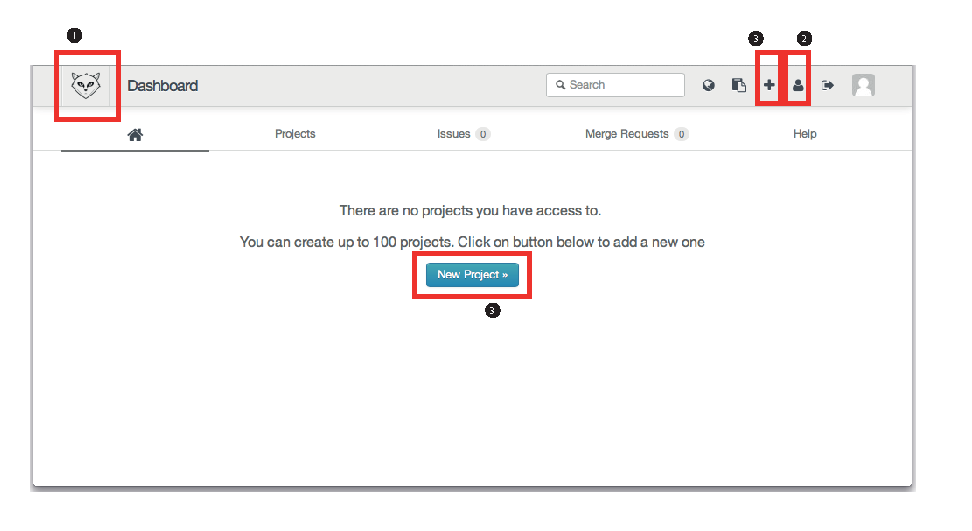
\includegraphics[width=15cm]{images/gitlab-first-login}}
\caption{First login to Gitlab. \protect\circled{1} The Gitlab logo (a sort of raccoon thing) will bring you back to the dashboard; useful if you get lost in gitlab's structure; \protect\circled{2} the user-profile allows you to add more information about yourself, and optionally connect up to Gravatar to give you a user icon; and \protect\circled{3} various ways to create a new project.}\label{figure:gitlab-first-login}
\end{figure}

Select thew `New Project' button from the icons at the top right. Enter \ttout{aboutme} as the project name, and hit `Create project'. You'll see a page similar to Figure \ref{figure:gitlab-new-project}. Notice that the `Git global setup' section contains the commands that you used in the previous section to set up your git configuration; so you don't need to do that again. There are also two other sections of code on how to `create repository' or use `Existing Git Repo?'. Ignore both of these for now and instead follow the instructions here (notice at the top of the gitlab page a warning that `You won't be able to pull or push project code via SSH until you add an SSH key to your profile' -- we need to fix that first). Click on the `add an SSH key' link (marked with \protect\circled{1} on Figure \ref{figure:gitlab-new-project}), which will take you to the SSH key upload page which looks something like Figure \ref{figure:gitlab-ssh}.

\begin{figure}
\centerline{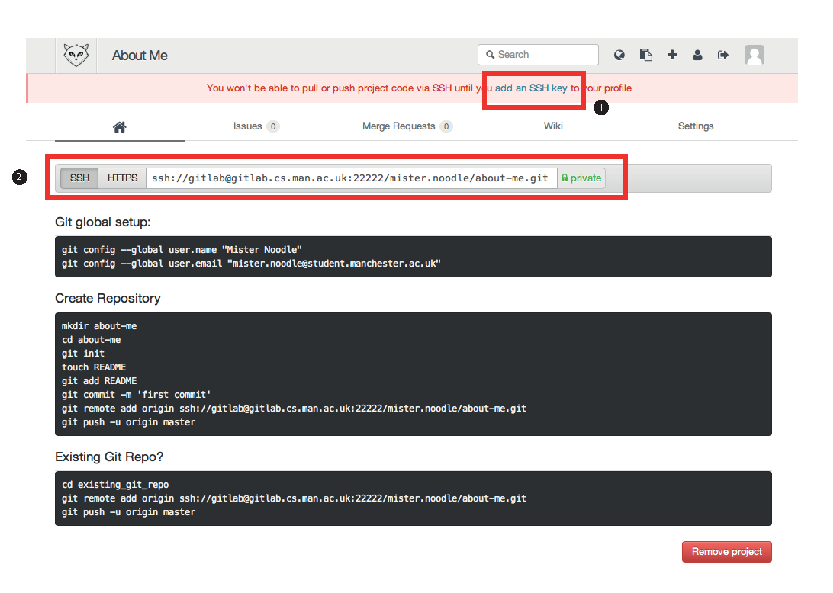
\includegraphics[width=15cm]{images/gitlab-new-project}}
\caption{Creating a new project in Gitlab. \protect\circled{1} You will need to use the  `add an SSH key' link to upload your public key before you can communicate between git and gitlab, and the URL given in \protect\circled{2} can be used from the command line to clone and push this project.}\label{figure:gitlab-new-project}
\end{figure}

\begin{figure}
\centerline{\includegraphics[width=13cm]{images/gitlab-ssh}}
\caption{Adding a SSH key to Gitlab. Once you have used \ttout{ssh-keygen} to create the key, paste the text into the `Key' box; if your key is valid then the title will be filled in for you.}\label{figure:gitlab-ssh}
\end{figure}


You'll now need to set up a means of securely identifying yourself to Gitlab from whichever machine you're using at the time; this is done by creating what's called a `ssh key'. In a terminal, type

\begin{ttoutenv}
ssh-keygen -t rsa -C "[YOUR UNIVERSITY EMAIL]"
\end{ttoutenv}

to create yourself a SSH key. When prompted `Enter file in which to save the key' just press return to accept the default, and the same for `Enter passphrase' twice.  For now don't worry too much about exactly what a SSH key is -- we'll just treat it as a way of identifying yourself to the Gitlab server. 

Look in a directory called \ttout{~/.ssh} and you'll find two new files have been created called \ttout{id\_rsa} and \ttout{id\_rsa.pub}. The first of these is the \textit{private} part of the SSH key that's just been generated for you, and you should keep this secret. The second of these is the \textit{public} part of the key, and this is the bit you need to hand over to gitlab for it to be able to identify you. Use the command

\begin{ttoutenv}
$ less ~/.ssh/id_rsa.pub
\end{ttoutenv}
% $
to display the contents of your public key. You should see something like:

\begin{ttoutenv}
  
  ssh-rsa  AAAAB3NzaC1yc2EAAAADAQABAAABAQDTfAF0KxG94oUJLUER5Ci5HaoEtdi8KI0S+
  iro3EvVkQebW2V3nCaCLAHLmgmINm/NFW5bvbUq7bu2CxFlVBEQqa1idZBLceXKRi1SFtG+
  EzFENyzZBsIDU0IhfQX4qyxgqe0A3ortyAwm2/+0neu74RT0YK3gQI+wyxsFFoCzbahiDJisK
  /vKmqvwowb/Rrl3OZpX9ZO3QA9lgILLVy3J4VpAhR+05MyuM/Bzh/pYk5NIQivedUEduIJXLOetj/
  UnxlH9WbEPEIiDPvzrkb3xI98rLRSlh2hH89nc1SUfVEhY62RQWN7sbXPu+fFck7Dom9wE/
  YAG66Dbl30OsmFh mister.noodle@manchester.ac.uk

\end{ttoutenv}


which starts with \ttout{ssh-rsa}, ends with your email address, and has a load of apparently random characters in between. Select this text (making sure you don't accidentally select any extra newlines or spaces either side of it) and 
Copy and Paste the whole of the SSH key into the `Key' box on the gitlab page. If you've done this correctly, gitlab will spot the email from your key and use this as the `Title' field, in which case just press the Save button. Gitlab will complain if it's not a valid key or has extra spaces or newlines at this point; if you're stuck here grab a demonstrator to help you. 

Once you've uploaded your public key to gitlab, you're ready to put your first bit of content into the `aboutme' project that you've just created. 

Click on the gitlab logo at the top left of the gitlab page to get back to the dashboard, and select the `aboutme' project that you created a moment ago.  Back at your terminal command prompt change to the directory called `aboutme' that you copied over from the Pi at the end of the last session; this should contain at least three files if everything has gone to plan: a bit of HTML about you, a photograph of your, and whatever image you drew using Inkscape (if for whatever reason you didn't get as far as that part in the last session, there's a default set of files you can use; copy them from \ttout{/opt/info/courses/COMP101/aboutme} into a directory called \ttout{aboutme} in your home directory and press on.)

\begin{note}
 Need to set this up in /opt/info
\end{note}

In your \ttout{aboutme} directory, type the following command:

\begin{ttoutenv}
$ git init
\end{ttoutenv}

which tells git that you're about to put this directory under its control; this is known as initialising a repository. Git will respond by telling you that it has `Initialized empty Git repository in ' followed by the full pathname of your \fname{aboutme} directory. 

Type
\begin{ttoutenv}
$ git status
\end{ttoutenv}

and you'll see a message from git that, amongst other things tells you that there are `untracked files' (these should appear in red). 

Now we need to tell git which files we want it to track for us. For each of the three files in that directory run a command along the lines of 

\begin{ttoutenv}
$ git add [FILENAME]
\end{ttoutenv}

% $

replacing [FILENAME] with each of the three file names in turn. Once you've done this, run \ttout{git status} again,, and this time you should see that there are a list of `Change to be committed' and all the files that you'd just added should appear in green. 

Now git knows which of the files in this directory you want to track (which in this case is all of them), we want to do our first `commit', which tells git that we've made a set of changes that we want to keep together: in this case the `changes' are to create the files in the first place; later one we'll go through a similar pattern of \ttout{git add} and {git commit} whenever we've done a set of changes that we think we are happy with. 

The \ttout{-m "Initial Commit"} part of the commit line gives git a label to associate with this particular commit, and it's traditional to put the message `Initial Commit' the first time you tell git about a new set of files. In future you'll be putting text here that summarises in human-readable form what changes you've made in this commit, but more on that later.

\begin{ttoutenv}
$ git commit -m "Initial Commit"
\end{ttoutenv}

Don't worry about what git's response means here, that will become clear as you learn more. Type \ttout{git status} once more and if everything has gone to plan you should see the response

\begin{ttoutenv}
# On branch master
nothing to commit (working directory clean)
\end{ttoutenv}

If you get a different message here, then something has gone wrong in one of the previous steps; don't worry, just call a demonstrator to help out. 

So to recap: in gitlab we've created a project called `aboutme' ready to accept some files, and in your home directory we've created a new repository (which happens to have the same name). The next step is to make an association between the repository in your home filestore, and the project on the gitlab server. 

Look back at the aboutme project's page on gitlab, and you'll see a box with a pair of controls labelled `SSH' and `HTTPS' followed by a fairly long URL (labelled with \protect\circled{2} in Figure \ref{figure:gitlab-new-project}) that is something similar to:

\begin{ttoutenv}
ssh://gitlab@gitlab.cs.man.ac.uk:22222/mister.noodle/aboutme.git
\end{ttoutenv}

Then enter the following command, copy-and-pasting the URL from the web page into the appropriate bit of commandline:

\begin{ttoutenv}
$ git remote add origin [GITLAB-URL-GOES-HERE]
\end{ttoutenv}

And finally to send this first version of the repository over to the gitlab server, enter

\begin{ttoutenv}
$ git push -u origin master
\end{ttoutenv}

which should respond with some variation of 

\begin{ttoutenv}
Counting objects: 3, done.
Writing objects: 100% (3/3), 216 bytes, done.
Total 3 (delta 0), reused 0 (delta 0)
To ssh://gitlab@gitlab.cs.man.ac.uk:22222/mister.noodle/aboutme.git
 * [new branch]      master -> master
Branch master set up to track remote branch master from origin by rebasing.
\end{ttoutenv}

To check that everything worked properly, run the command \ttout{git pull} (note that you won't need to put the \ttout{-u origin master} bits after git pull from now on), and you should get the response:

\begin{ttoutenv}
Everything up-to-date
\end{ttoutenv}

Again, if something has gone wrong and you can't see what, grab a demonstrator. 

Go back to the gitlab page in your browser, and select the dashboard by clicking on the gitlab logo at the top left. On the right, you should see your `aboutme' project; you should see a history of what's happened to the project so far which will include you joining the project, and `pushed a new branch'. Select the `Files' page from the menu near the top of the page, and you should see a list of the three files that you've added so far. 

To recap; you've now created your first local repository (the directory in your filestore called \fname{aboutme}), added and committed your first `changes' (which in this case meant telling git about the existence of the files you want to track in the first instance), and synchronised these files with a remote repository hosted by the School's gitlab server. That may have all seemed like rather hard work, but now you're set up to use the respository for real, and things get a bit easier from here on. 

\subsection{Cloning a repository}

Imagine now that after a particularly hard day's work, you've accidentally deleted your \fname{aboutme} directory. In fact, let's just do that now. Change to your home directory, and type

\begin{ttoutenv}
$ rm -rf aboutme
\end{ttoutenv}

which will recursively delete the \fname{aboutme} directory and all its contents without prompting you for anything. Check that the directory has gone using \ttout{ls}. And now let's fetch it back from our remote gitlab repository (which is nicely backed up for you by the School's IT Services, so you can be safe that nothing bad will happen to it). Type

Find the ssh URL for the project in gitlab, and paste the URL into the \ttout{git clone} command:

\begin{ttoutenv}
$ git clone [PROJECT-URL-GOES-HERE]
\end{ttoutenv}

%$
You should see a response that starts with `Cloning into' followed by some other lines of stuff, and your `aboutme' repository should re-appear, complete with all its contents.

Change into the \fname{aboutme} directory, and issue \ttout{git status}, which should reassuringly tell you that there is `nothing to commit (working directory clean)' (which means `you've not made any changes since the last time you touched this repository'). 

Now edit the HTML file to make some small change (it can be anything you'd recognise as a change, doesn't matter what), and once more type \ttout{git status} to see what git things has happened.

Git should tell you that your HTML file is now `modified'. You've now got two options:
\begin{itemize}
\item Let's say you want to throw away the change you've just made  (imagine it was a much more complex edit
  than the one you've just  made, and you're not happy with it). To do this you can run
  \ttout{git checkout -- [FILENAME]} to revert the file back to the
  last version you committed.
\item Alternatively, if you want to keep the change you've made, you can run \ttout{git add [FILENAME]}
  followed by \ttout{git commit [FILENAME] -m "[A DESCRIPTION OF WHAT YOU CHANGED]"} to commit the file to your local repository. 
\end{itemize}

When you want to preserve your commit on the server (for example, because you've finished for the day and want to pick up the files when you get home, or because someone else in your team needs to see your changes, or because you've finished a nice complete self-contained bit of work), you can then syncrhonise your local repository with the project hosted on gitlab. To do this, you just need to issue 

\begin{ttoutenv}
$ git push
\end{ttoutenv}
% $

and any commits that you've made will get pushed to the gitlab server. 

Experiment now by making a few more changes to the contents of your aboutme directory; add an extra file or two, and modify their content. Use \ttout{git status} regularly to make sure that git reflects what you're doing. Keep in mind the following principles:

\begin{itemize}
\item When you've modified one or more files and want git to know about these changes, use \ttout{git add} to tell git to track the changes to those files.

\item You don't need to use \ttout{commit} after every \ttout{add};
  you can safely bundle up a set of \ttout{add}s in a single commit,
  (when you start working on more complex projects you'll find that is often the case). A    commit should represent a coherent set
  of changes to your work that you are recording for a particular
  reason. You should summarise this reason in the log entry message
  that follows the \ttout{-m} switch on the \ttout{git commit} line, so that
  later on you can see what the different commits were for.

\item When you have finished a particular job, or need to move to another machine, use \ttout{git push} to synchronise the changes you've made to your local repository with the gitlab server; then these changes can be picked up from elsewhere or (later on when you're doing project work) by other people in your team. 
\end{itemize}

After you've played around with \ttout{add}, \ttout{commit} and \ttout{push} a few times, try using the \ttout{git log} command to see the history of what you've done. You should also be able to see this history in gitlab as well --- but we'll leave you to explore the gitlab interface to find out how to do that. 

\subsection{Using git/gitlab to transfer files between machines}

Clone and pull. 

\subsection{Using git to publish content to a webserver}

By now you should have a basic idea of how you can use git to track modifications to files, and how gitlab can help you move files between machines (and when the time comes, an inkling of how it can be used to share content with other members of your project). To finish off this session we're going to show you how to use git and gitlab to manage changes to a website.

In your previous experiments with the simple Python webserver and Apache on your Pi, you've been creating and manipulating files in a directory that is directly visible to the web server. So every time you change and save a file, that change becomes immediately visible to the web server, and therefore to anybody viewing the web page. This was great as a way of showing you what a webserver is really doing behind the scenes, but it's not a good example of how `real world websites' are managed. A real website typically consists of lots of interlinked pages, and changing just one file at a time would mean that during the period you're making edits the content of the site could become inconsistent. Often what you really want to do is to make a whole set of changes to different files, and then only when you're happy that you've made all the changes you need, to make the updated site visible to users. Of course you could do this by taking a copy of the website's files, editing them `offline' somewhere, and then copying them back manually in to the right place on the web server's filestore---but hopefully by now you can see how git/gitlab can help out here.



\section{And finally . . . Blackboard!}
\label{sec:blackboard}

You won't be using it for this course-unit, but for your other course-units you may be using a different Virtual Learning Environment - \textsf{Blackboard}. The usual way to access \textsf{Blackboard} is via the \href{https://my.manchester.ac.uk}{\emph{My Manchester}} page at \urlnop{my.manchester.ac.uk}, and then use the \emph{'My Blackboard'} tab. There is also a plentiful supply of information about how to use Blackboard available online.



\renewcommand{\chaptername}{COMP10120 Lab Session}
\setcounter{chapter}{0}
\coursecode{COMP10120}
\chapter{Academic Malpractice Awareness: DRAFT VERSION}

\notesurl{desktop3}

\begin{note}
  This is where the script for the Academic Malpractice Awareness and Health and safety exercise goes

\end{note}


\chapter{Programming the shell}

\begin{note}
  This is where the script for the shell script exercise goes

\end{note}



% \usepackage{graphicx}
% \usepackage{palatino}
% \usepackage{url}
% \usepackage{hyperref}

% %\usepackage{a4-mancs}

% \usepackage{handout}

% \begin{document}
\newgeometry{a4paper}
\setlength{\parskip}{\parskipdefault}
\setlength{\parindent}{\parindentdefault}

\chapter{Report writing and Digital Typography}
\begin{refsection}
  
  \minitoc

  \notesurl{latex-exercise}

\section{Introduction}

\LaTeX\ is a document preparation system that is fundamentally
different to anything that you are likely to have seen before. It's
used worldwide by publishers, academics and scientists.

\LaTeX\ was written by Leslie Lamport, an American computer scientist now working at Microsoft Research.  It's actually built on top of another system called \TeX, a computer typesetting system designed by one of the world's most influential Computer Scientists, Donald Knuth of Stanford University. Knuth has said that he designed \TeX\ for ``the creation of beautiful books---and especially for books that contain a lot of mathematics.'' \citep{knuth1984}. Figure \ref{figure:knuthlamport} shows what these eminent men look like.

  
So what's the purpose of \LaTeX ? It's purely a layer of software to make \TeX\ easier to use in everyday situations. This is a good idea, because although \TeX\ is amazingly powerful, it operates at a very low-level, which makes it hard for non-expert users.

\begin{figure}[hb]
  \centering
     \includegraphics[height=6cm]{images/knuth.png}
\quad\quad  \includegraphics[height=6cm]{images/lamport.png}
\caption{Don Knuth and Leslie Lamport.}\label{figure:knuthlamport}
\end{figure}

\subsection{Pronunciation}
\label{sec:pronunciation}
  The name \TeX\ is intended by its creator to be pronounced with the final consonant as in the word loch or the name Bach, but English speakers often pronounce it like the first syllable of technical. The first syllable of \LaTeX\ is pronounced as in 'lay'\footnote{The Greek prefix `tex' means `art' as well as `technology', so it's a very nicely chosen name for a piece of software that produces such beautiful output. Knuth explained \citep{knuth1984} that one should ``pronounce the X of TeX as a Greek chi, not as an `x', so that TeX rhymes with the word blecchhh.''. We're not too sure that helps much, unless you are confident in your pronunciation of the word `blecchh'. Maybe it's an American thing.}.


\section{Why \LaTeX?}
\label{sec:why}
 Before we go any further, why do we think \LaTeX\ is important for you---a Computer Science student---to know about? Here are some reasons, in no particular order.

\begin{itemize}
\item \LaTeX\ and \TeX\ are superb examples of Computer Science in action. \TeX\ was designed by Knuth from first principles---in other words, ``from scratch''.  \TeX\ is actually a programming language, and \LaTeX\ is a set of functions defined in the \TeX\ language. The \TeX\ ``compiler''  (the source code is publicly available in C and Pascal)  reads a \TeX\ program and outputs documents. \TeX\ is completely self-contained and designed to be portable to any computer architecture. (For example, it implements its own stack and heap (with garbage collection), and it does fixed-precision arithmetic). 
\item \LaTeX\ is a new, interesting, way for you to think about preparing documents. 
\item \LaTeX\ has a practical advantage for the writer, in that it helps you think more about \emph{what} you want to write, rather than worrying about \emph{how it looks}.
\item \LaTeX\ is a powerful tool for professional scientific documentation, and as a Computer Scientist, you should know about it.
\item \LaTeX\ files are just `plain text', so can easily be created programatically. For example,  the slides used for \courseunit{COMP16120} are generated automatically from the source of John's book; both are typeset using \LaTeX. The program \texttt{labprint} also produces its output using \LaTeX, using information drawn from XML configuration files and ARCADE.
  
\item Using \LaTeX\ is actually quite satisfying, and the quality of its output may surprise you.
\end{itemize}

In this lab session you are going to write several short  documents using \LaTeX. You could also write brief notes in your logbook about how \LaTeX\ works and what commands you used inside the source of your documents.

Please complete the exercises in your \fname{COMP10120/ex3} directory. When you have completed as much as you are going to do, you should run \texttt{submit} and (when next in the School) \texttt{labprint}.

\section{Some history: printing mathematics}

Mathematics is hard to print, on paper, and on the Web (many websites resort to GIF or JPG images of maths formulae, which usually look horrible. \wikipedia{MathML}{MathML} provides another approach, but it is not yet widely used).

In the days before computers, books and newspapers were printed with ``movable type'', made from lots of little blocks of metal each with letters, numbers and symbols standing in relief, which, when inked, left an impression on the paper (see Figure \ref{figure:movabletype}). The job of the printer (the printer here, of course, being a person, not a bit of electronics) was to gather together all the blocks in the right order between two horizontal strips of wood to create a line of the document, and then to assemble all those lines from top to bottom of a page. Thus the term `type setting': an incredible task, when you think about it. In the printer's workshop, by the way, the blocks of metal were stored between jobs in wooden boxes called `cases'. Letters like a, b and c were stored in one case; letters like A, B, and C were stored in a case sitting on top of that. So, a lower case, and an upper case. These terms may ring a bell.

\begin{figure}
\centerline{\includegraphics[width=12cm]{images/movable-type.png}}
\caption{On the left, a piece of cast movable type in the Garamond font. On the right, a case of cast metal type pieces and typeset matter in a composing stick. The text reads `The quick brown fox jumps over the lazy dog and feels as if he were in the seventh heaven of typography together with Hermann Zapf, the most famous artist of the' (this document is typeset in a font called Palatino, created by Hermann Zapf. You may have also seen 'Zapf Dingbats' in the font lists of various desktop applications. Now you know why.)} \label{figure:movabletype}
\end{figure}

As technology progressed, machines controlled by typewriters would mechanically juggle the blocks into the right order. This conceptual model is the basis on which \TeX\ operates. Only now, the metal blocks are little pieces of data, arranged into data structures. 

The one thing that traditional printers hated was dealing with the typesetting of mathematics, and they would charge extra to do it. It was incredibly fiddly: to get the equations looking right they had to squeeze in extra bits of metal horizontally and vertically. 

When computers entered the printing world, attempts to print mathematics were limited by the printing technology available. It took a long time to reach the point where computers could typeset mathematics beautifully, and that was the outstanding achievement of Knuth's \TeX.

Let's look at a quick example of the quality you get from \LaTeX, with a very simple formula that you'll recognise:

\[ x = \frac{-b \pm \sqrt{b^2-4ac}}{2a} \]
%
We'll revisit how \LaTeX\ typesets mathematics in Section~\ref{mathssection}.

\section{To WYSIWYG or not to WYSIWYG?}
Up until now, you have probably used wordprocessing applications such as Microsoft Word to create essays, letters and other (probably fairly short) documents. You most likely know that the majority of modern word processors use a paradigm called WYSIWYG, or What You See Is What You Get, which means that you can modify the visual style of the document you're working on by selecting the relevant bits, and then choosing different attributes such as font size or colour using a GUI. In many ways this seems like such a sensible and obvious way of doing things, that you might be wondering why it even has a special name. The reason is a historical one: in the early days of computing, long before graphical window managers became the norm, and when all you could display on screen was fixed-width ASCII text in whatever the system's default font was, wordprocessors (e.g. Figure \ref{figure:wordperfect}) only allowed you to format documents by using special sequences of characters to cause particular effects. But these effects were only visible when the document was printed. So if you wanted a word to appear in \textbf{bold text}, in the wordprocessor you might write something like \texttt{[bold]hello world[/bold]}: what you saw on screen was \emph{not} a direct reflection of what appeared on the printed page. If you've written any HTML, however, this process of `marking up' text may be familiar, see, for example Figure~\ref{figure:helloworld}. As computers moved to displays able to draw things other than raw characters on screen, wordprocessors became capable of using multiple fonts and styles, as well as graphics, and a new generation of applications appeared where what you saw on screen \emph{was} an accurate reflection of how it would appear when printed: what you see (on screen), is what you get (on paper). 

\begin{figure}
\centerline{\includegraphics[width=12cm]{images/wordperfect.png}}
\caption{A screenshot of Wordperfect 5.1, running in Microsoft DOS circa 1989.}\label{figure:wordperfect}
\end{figure}

\begin{figure}

\begin{verbatim}
                \documentclass{article}
                \begin{document}
                \textbf{Hello world}
                \end{document}
\end{verbatim}
\center{(a)}
\begin{verbatim}
                <html>
                  <body>
                     <b>Hello world</b>
                  </body>
                </html>
\end{verbatim}
\center{(b)}

\caption{Examples of the words `hello world' in bold text typeset (a) \LaTeX\ and (b) HTML}\label{figure:helloworld}
\end{figure}


The huge advantage of WYSIWYG is that it's really easy to understand what's going on, and most people can create reasonably nicely formatted documents with relatively little effort. For short informal documents, one-off letters, memos and such, WYSIWYG works quite nicely. But if you've ever tried writing anything much longer, or that includes images and tables, you may have already started to see where the paradigm breaks down. For example, if you write ``Figure \ref{figure:menandcheeses} on page \pageref{figure:menandcheeses}  shows a picture of some men looking at cheese'', but then later on edit your document to include some more text at the start, and a new picture of a some broccoli (as in Figure \ref{figure:broccoli}), you'd have to search through your report to find all mentions of `Figure \ref{figure:menandcheeses}' and `page \pageref{figure:menandcheeses}' and manually update them to reflect the new numbering. This might be fine if you have two figures and five pages; but for a hundred-page report containing lots of pictures, you can see how this becomes tedious and error prone very quickly. 

\begin{figure}
\centerline{\includegraphics[width=10cm]{images/men-and-cheese.jpg}}
\caption{Some men, possibly Dutch, looking at cheeses.}\label{figure:menandcheeses}
\end{figure}

\begin{figure}
\centerline{\includegraphics[width=10cm]{images/broccoli.jpg}}
\caption{Some broccoli.}\label{figure:broccoli}
\end{figure}

\section{Style and content}

The other thing about WYSIWYG is that it puts you entirely in control of the visual layout and style of your article, and this isn't necessarily a good thing for two reasons. First, it means that instead of focusing on the content and structure of what you're writing, it makes it easy to get distracted by tinkering with the layout and style. And although layout and style are of course important if you want to create a professional-looking document, they are definitely always secondary to content and structure. Second, it means that you are, well, entirely in control of the visual layout and style of your article. And although it might not be obvious up-front, such control is not necessarily a good thing unless you really know what you're doing (and unless you are a talented graphic designer with a deep understanding of typography, you almost certainly don't\footnote{Don't take this personally; we're in the same boat. If you think that this document is nicely formatted, that's all down to \LaTeX, not us!}). Creating documents that are aesthetically pleasing and easy to read is rather a specialist skill with its origins going all the way back to Caxton's invention of the printing press in the fifteenth century.  Over the years, typographers have honed their skills, arriving at complex rules and heuristics that determine the optimum number of characters on a line, ideal relative and absolute font sizes, spacings, margins, figure placement and so on that lead to attractive---and most importantly---readable documents. You could of course learn all these rules, and make sure you implement them manually using your favourite WYSIWG editor, but that's not what a Computer Science degree is about. The \LaTeX\ system implements many of these rules, making decisions for you about the best way to lay your document out on the page. This allows you to concentrate on creating good quality content, safe in the knowledge that \LaTeX\ will do a good job of presenting it out for you. The idea of separating out `content' from `presentation' is something you'll encounter many times during your studies of Computer Science. You'll see it again in a fairly obvious way soon when you come to writing some HTML and CSS in Phase 3 of this course unit: but the concept of distinguishing between a `model' and a `view' will reappear in increasingly subtle ways throughout your degree. 

\section{The right tool for the right job}

To avoid any  misunderstanding, we are not at all trying to claim that \LaTeX\ is ``better'' than Word (or similar), just that it's ``different'', in fact, ``extremely different'', both in its capabilties, and its conceptual model. One of the key skills that any professional needs to learn is to be able to choose the right tool for the right job. If you're going to open a coconut, you'll probably use a corkscrew, not a pneumatic drill. Similarly, if you're writing a quick letter, or making a DO NOT DISTURB sign, you'll probably want to use a quick WYSIWYG tool like Word. If, however, you're writing a technical document, perhaps with some maths, or a 3rd Year Project Report, or an article you want to get published, then you'll probably want \LaTeX.  You might see analogies with programming here---and which languages are best suited to which jobs.

\section{Getting started}

The downside of using a non-WYSIWYG system such as \LaTeX\ is that there is rather more to understand and master before you can get going. You will have probably spotted that this is a recurring pattern: to perform certain tasks, we often have the choice between two approaches: the first (in this case the WYSIWYG way) allows you to get going straight away as a novice, but doesn't allow us to `grow' much expertise to get better and faster, and as you try to do more complex things, you discover problems and limitations that are hard to overcome; the second is inherently more powerful, but requires you to invest time and effort before you can get started. Wordprocessors and file browsers fall into the former category; \LaTeX\ and use of the command line into the latter.

By the time you get to write your third year project report, you will almost certainly want to use \LaTeX. Indeed, that might well be the point at which you will gain the most benefit from it throughout your studies here. What you do not want is to be having to learn \LaTeX\ at that point--it will be challenging enough without that extra burden. So, we are embarking you on a programme of learning \LaTeX\ more gradually.

%Start by creating the directory $HOME/COMP10120/ex4 and make it your current one. 

\section{The exercises}


\exercisess{A closer look}
%\subsection{Exercise 1}
\label{sec:exercise-1}


Fire up your favourite editor, enter the following text (it's important that you enter it exactly as it is below for now), and then save it as a file called \fname{fire-and-ice.tex} (in case you're wondering, it's the first line from a short poem called `Fire and Ice' by American poet Robert Frost \citep{frost1923}; the whole poem is on the \href{http://www.poetryfoundation.org/poem/173527}{Poetry Foundation website} if you're interested.)

\begin{verbatim}
\documentclass[a4paper]{article}
\begin{document}
Some say the world will end in fire,
\end{document}
\end{verbatim}
%
Next, run the command \texttt{pdflatex fire-and-ice.tex} (for now it's sufficient to say that pdflatex invokes \LaTeX\ to create a PDF file as the output; the full story is a bit more complicated.)

\LaTeX\ will process your file, and print out a surprisingly large amount of text into the shell window as it does so. If all is well, the last two lines printed out will be something like:

\begin{verbatim}
Output written on simple.pdf (1 page, 11853 bytes).
Transcript written on simple.log.
\end{verbatim}
%
after which \LaTeX\ will return you to the command prompt. If you've made a mistake typing in the file, \LaTeX\ will stop part way through processing your work, and display an error (possibly, quite an obscure one) and show a `?' prompt. The best thing to do at this stage is to press \ctrl{d}, or \ttout{x}, to tell \LaTeX\ to give up trying to process your file. Then fix the mistake, and try again.  

If you now list the contents of the directory, you should see that a file called `fire-and-ice.pdf' has been created (along with two other files called `fire-and-ice.aux' and `fire-and-ice.log' both of which we will ignore for now). Use one of the PDF readers (such as \cmdname{evince}) to look at the content of `simple.pdf'.  Admittedly, it's not the most exciting result; if everything has worked properly so far, you should see single-page document with the words `Some say the world will end in fire,' a little way down from the top of the page\footnote{If you have been carried away with the sheer excitement and joy of learning to use \LaTeX\, and improvised the text rather than typing the first line of `Fire and Ice' as requested, please go back and change it now: it really is important that you use exactly that text. Really, it is. That's better. Thanks.}.

But now look more closely. A lot more closely\ldots really zoom in. See anything interesting?

Even for this very short document, \LaTeX\ has taken a fairly sophisticated typographical decision on your behalf and `ligated' (which is typo\-graphy-speak for `joined') the `f' and the `i' in the word `fire'; the spacing between the characters has been subtly altered so that the dot above the `i' and the blob on the end of the curvy bit (the `arc of the stem', if we're being formal) on the top of the `f' join together to form a single shape called a \emph{ligature}. Why? Because having two blobs side by side simply looks a bit clumsy as you can see in Figure \ref{figure:twofires}. To make this decision, \LaTeX\ has had to know a lot about the fonts being used (not all `f's in all fonts have a blobby end; not all `i's in all fonts have a round dot that would merge nicely with the blobby bit on the end of an `f', and so on). There's a reasonable chance that you've never heard of ligated characters before---it is, after all, a fairly specialist thing. And there are hundreds of other obscure but important `rules' of typography that go to make professionally typeset documents look good\footnote{Look up `kerning', `combining characters' and `serif' on Wikipedia for starters. And if you're really keen, Donald Knuth's fascinating and compendious book `Digital Typography' \citep{knuth1999} has an entire chapter dedicated to the joys of the letter `S'. Probably best not to bring this subject up at the pub though, or at parties. Unless they are very specialist parties.}. Individually, they might not be obvious or hugely important, but collectively and subliminally they make the difference between something that looks just-about-acceptable (like most things written using wordprocessors) and things that stand out as looking really professional (you might want to remember this when it comes to putting your CV together.)

\begin{figure}[htbp]
\centerline{\includegraphics[width=6cm]{images/fireandfire.png}}
\caption{The word `fire' typeset by (a) Microsoft Word 2011 without ligated characters, and (b) by \LaTeX\ showing the ligation of the characters `f' and `i'.}\label{figure:twofires}
\end{figure}
%
But that's enough about the typography of the word `fire' for now. Let's put together something more substantial. 

\exercisess{A larger example}
%\subsection{Exercise 2}
\label{sec:exercise-2}

 Create yourself a new file, called \fname{sections.tex} by copying \fname{fire-and-ice.tex}. In \fname{sections.tex}, replace the line of poetry with the text from Figure \ref{figure:bleakhouse} (which contains the first three paragraphs of Dickens' novel, `Bleak House' \citep{dickens1852}).

\begin{figure}[tbp]

\begin{quote}

  \itshape
  \raggedright
  
London. Michaelmas term lately over, and the Lord Chancellor sitting
in Lincoln's Inn Hall. Implacable November weather. As much mud in
the streets as if the waters had but newly retired from the face of
the earth, and it would not be wonderful to meet a Megalosaurus,
forty feet long or so, waddling like an elephantine lizard up Holborn
Hill. Smoke lowering down from chimney-pots, making a soft black
drizzle, with flakes of soot in it as big as full-grown
snowflakes--gone into mourning, one might imagine, for the death of
the sun. Dogs, undistinguishable in mire. Horses, scarcely better;
splashed to their very blinkers. Foot passengers, jostling one
another's umbrellas in a general infection of ill temper, and losing
their foot-hold at street-corners, where tens of thousands of other
foot passengers have been slipping and sliding since the day broke
(if this day ever broke), adding new deposits to the crust upon crust
of mud, sticking at those points tenaciously to the pavement, and
accumulating at compound interest.



Fog everywhere. Fog up the river, where it flows among green aits and
meadows; fog down the river, where it rolls defiled among the tiers
of shipping and the waterside pollutions of a great (and dirty) city.
Fog on the Essex marshes, fog on the Kentish heights. Fog creeping
into the cabooses of collier-brigs; fog lying out on the yards and
hovering in the rigging of great ships; fog drooping on the gunwales
of barges and small boats. Fog in the eyes and throats of ancient
Greenwich pensioners, wheezing by the firesides of their wards; fog
in the stem and bowl of the afternoon pipe of the wrathful skipper,
down in his close cabin; fog cruelly pinching the toes and fingers of
his shivering little 'prentice boy on deck. Chance people on the
bridges peeping over the parapets into a nether sky of fog, with fog
all round them, as if they were up in a balloon and hanging in the
misty clouds.

Gas looming through the fog in divers places in the streets, much as
the sun may, from the spongey fields, be seen to loom by husbandman
and ploughboy. Most of the shops lighted two hours before their
time---as the gas seems to know, for it has a haggard and unwilling
look.

\end{quote}

\caption{Some sample text from the opening of the Dickens' novel `Bleak House' \citep{dickens1852}.}\label{figure:bleakhouse}
\end{figure}

Edit the text to make sure that there is a blank line between each of the three paragraphs (it's not enough that each paragraph starts on a new line of its own, there has to be an empty line in between them). That's how paragraphs are distinguished in \LaTeX\ (in fact, it doesn't matter how many blank lines you put as long as there is at least one\ldots for the most part \LaTeX\ ignores spare whitespace). Now type a paragraph of gibberish by randomly hitting keys on the keyboard, and putting spaces in to make `words' in the text file. You should end up with something like the following, but about three times as long (don't cut and paste this from here\ldots it's important that you actually create some unique gibberish yourself!):

\begin{verbatim}
Oisjdf oqweqwe oi soijs hbweo kbsd oijsdf 
oijqwknpiouh iusbdfspb sifuhygwqeb usgweijf 
blimqwoq oieuerwefwiu aokqjw uioshiufds 
qiqks odfubfi psdiweneq.
\end{verbatim}

Be careful at this stage to only include letters (uppercase and lowercase), commas, full-stops and perhaps numbers in your gibberish text: if you use any other symbols, you may upset \LaTeX. 

Next go to the website \href{http://www.lipsum.com/}{http://www.lipsum.com} and follow the instructions to generate yourself three paragraphs of what's called `Lorem Ipsum' text. Copy and paste that text into your \LaTeX\ document too (don't worry about what it means at this stage), again making sure that you have a blank line between the paragraphs.

Re-run \texttt{pdflatex} and look at the resulting \fname{sections.pdf}. Again, at first glance, there's nothing hugely exciting going on here: the text from your \fname{.tex} file has been assembled into a (probably) two page PDF document. But in fact quite a few things have happened: 

% \begin{note}
%   Why don't we indent pars? Because we have lots of short ones?
% \end{note}

\begin{itemize}
\item The blank lines that separate the paragraphs in your source file are gone, and instead \LaTeX\ has indented the first line of each paragraph. There's nothing profound here about the decision to indent paragraphs rather than (say) to leave a gap between them (so called `block paragraphs'); it's just \LaTeX's default paragraph style, and can be changed easily enough.\footnote{Though apparently, there is some evidence in \cite{tinker63} that indented paragraphs increase readability}
\item There are page numbers at the bottom of each page. This is a very sensible default, allowing you in meetings to ask people to ``turn to page 4'' and so on (it's a bit odd, and a source of some annoyance, that most wordprocessors don't do this by default too). But you can easily switch page numbers off, change their style or move them elsewhere if you need to. 
\item The text is `fully justified' so that it's flush on both the left and right hand edges.
\item Certain words that fall at the end of lines have been hyphenated, even if they weren't originally split by hyphens in the source text.
\end{itemize}

These last two points about justification and hyphenation might seem utterly trivial, but getting these factors right turns out to be an important part of making readable documents; readability is not just about which font you choose, but about how the characters and spaces are distributed on each line. It's something that you will have seen happen so often in professionally typeset materials that you'll have taken it for granted, and you may not have spotted that it doesn't happen in quite the same way when you use a wordprocessor. The principle behind justifying text seems easy enough at first glance: you simply have to take any `left over' space that would be at the end of a line, and redistribute it between the words in some way to `space them out' a bit more so that they take up all the available horizontal room. But it turns out to be much harder than it seems, and all the simple ways you might think of for doing this on a per-line basis give results that are visually quite unsatisfactory, with nasty patterns made up of neighbouring whitespace appearing in the layout and ruining everything. The added complication here is that to do the optimum job of shuffling the words round on their lines, you really need the flexibility of being able to hyphenate words to give you extra space on lines that would otherwise be tightly packed with characters. But if you hyphenate words badly, by breaking them in inappropriate places, or do it too often then that makes the text hard to read too. It's all deeply inconvenient and inter-related. The best solution to this aesthetic conundrum so far was developed by \cite{SPE:SPE4380111102} and later improved by Frank Liang during his PhD research \citep{liang}, and it's a technique that tries to optimise the layout of whole paragraphs rather than individual lines. The algorithm takes into account all manner of different things: language-specific character patterns, the number of consecutive lines that end with hyphens, the word `tightness' on each line\ldots any many others. The details don't really matter here, but the really important thing insight is that you get better results by working on a bigger chunk of the document (in this case a paragraph at a time) rather than trying to independently optimise lots of small bits (say, lines) and hoping that the result of joining them all together turns out nicely. This idea of optimising things `globally' versus `locally' is something you'll see many times throughout your Computer Science degree; watch out for it in all the algorithms courses.

This highlights a fundamental difference between the WYSIWYG para\-digm and the way that documents are produced using \LaTeX. As we've seen, small changes down at the the level of individual characters can have fairly large knock-on consequences for the optimal layout of a document: changing one letter for another affects the length of a line, which in turn affects the hyphenation options, which then affects the length of a paragraph, which means that the best place for a figure that was on page 99 might now on page 100, but that means that all references to `page 99' now need a bit more room to account for the extra digit which means that the some line lengths have changed which means\ldots well, you get the idea. It's more complicated that it first seems. \LaTeX\ gets to see the \emph{whole of your document at once}, and can therefore make decisions about how best to hyphenate lines,  position figures or whatever else it likes \emph{before} it shows you the results; so it can make solutions that are optimal for the whole document, as well as looking at details such as ligated characters. Wordprocessors can't afford to do this since it would be deeply distracting if every time you typed a character, the whole layout of the document flapped around in front of your eyes. Wordprocessors can only sensibly make little optimisations at a local (probably per-line level). It's not that wordprocessors are rubbish, or that the people that programmed them were lazy: it's a fundamentally different way of working, and knowing the pros and cons of the different approaches will help you pick the right tool for the job. 

You may have noticed that actual text in your document (and in fact, this one) takes up a (perhaps) surprisingly narrow horizontal region of the page. This last `feature' might seem odd at first, but it illustrates another important typographical point that you may never have thought of before: reading long lines of text is hard, because your eyes find it hard to move in a completely straight line as they scan from left to right. So the longer the line of words, the more you have to work to keep your eyes from accidentally drifting up or down onto a neighbouring line (perhaps you've experienced the phenomenon of accidentally re-reading the same line over and over as your eyes get tired). It may never have occurred to you, but most books have relatively short lines of text; and those that use large pages often split text into several columns so that individual lines are kept relatively short. The widely trusted book ``The Elements of Typographic Style'' \citep{bringhurst92} makes the following assertion:

\begin{quote}
\emph{
``Anything from 45 to 75 characters is widely-regarded as a satisfactory length of line for a single-column page set in a serifed text face in a text size. The 66-character line (counting both letters and spaces) is widely regarded as ideal.''}
\end{quote}

\LaTeX\ knows about this issue, so made a sensible default decision for you. You may have noticed that there is a subtle difference in appearance of this chapter from previous ones: the lines are shorter and paragraphs are indented. We wanted to use the default \LaTeX\ layout for this chapter, but changed it for earlier chapters in an effort to save paper.

There's one last unusual thing to note: your paragraph of gibberish text in between the real words from Bleak House and the Lorem Ipsum almost certainly stands out and looks really quite odd (it might even have confused \LaTeX's hyphenation rules enough to have ended up with one or more lines sticking out proud of the right hand margin).  Let your eyes relax so that your vision blurs for a moment: you can still probably spot that the gibberish paragraph looks out of place. It's quite likely that you even found creating the gibberish unexpectedly hard. The interesting thing here is that as humans, we spend so much time reading and writing `proper' natural language that we become attuned to the patterns of letters words and the underlying `rhythm' of our written language that its very hard to artificially reproduce something that looks plausible; the frequency of the letters you chose by randomly hitting keys, and the length and patterns of the words you put in place most likely don't match the natural patterns of real languages, so they just look plain wrong.  Curiously the Lorem Ipsum text that you got from the website probably doesn't look so bad, in spite of it not being made up of real words. But that's not surprising since `Lorem Ipsum' is specifically created to be used as a placeholder for real text when typesetting. While the words are meaningless Latin-like things, their length, and the distribution of characters and word lengths are chosen to mimic patterns in real language.

% \exercisess{Creating document structure}
% %  \subsection{Exercise 3}
% \label{sec:exercise-3}

Next let's give our document some structure by dividing it up into sections. On the line before Bleak House starts, add the command

\begin{verbatim}
\section{Bleak House}
\end{verbatim}
%
making sure it appears on a line of its own. Then just before your paragraph of gibberish, put similar a similar instruction (again, on its own line), and then create a final section before the Lorem Ipsum. Rerun pdflatex and look at the results. You should see the section headings appear in the appropriate places in the PDF, automatically having been given section numbers. Experiment by adding in a couple of sub-sections towards the end of the document using the  \verb|\subsection| command, which like \verb|\section| command above takes as a parameter some text in contained in wiggly brackets. 

Now, at the top of your document after the \verb|\begin{document}| line and before the command defining the first section, add the following two commands, each on their own line:

\begin{verbatim}
\tableofcontents
\newpage
\end{verbatim}
%
  Re-run pdflatex \emph{twice}, and check that the effect is what you'd expect. You need to process the source twice because on the first run, \LaTeX\ gathers and stores information about what to put in the table of contents, and only creates it on the second run.


\section{Common formatting features}

Before we give you some more exercises to do, here is a brief introduction to some commonly used features of \LaTeX.

\subsection{Enumerated and bulleted lists}

Creating bulleted or numbered lists in \LaTeX\ is straightforward, and is done like this:

\begin{verbatim}
\begin{enumerate}
\item My first item
\item My second item
\item The last thing on my list
\end{enumerate}
\end{verbatim}
%
You must make sure that you both \texttt{begin} and \texttt{end} your list, and that each item is terminated by a newline. Changing `enumerate' to `itemize' gives you a bulleted rather than numbered list (note the American spelling of `itemize').  

\subsection{Bold and italic text}
Text can be typeset in \textbf{bold} font using the \verb|\textbf|, and \textit{italics} using \verb|\textit| as in the example below:

\begin{verbatim}
Some say the \textbf{world} will end in \textit{fire},
\end{verbatim}

\subsection{Cross referencing}

\LaTeX\ allows you to cross-reference almost anything in the document, which includes sections, sub sections and figures. To use the cross-referencing feature you simply insert the command 
\begin{verbatim}
\label{mymarker}
\end{verbatim}
at the point in the document you want to refer to, and then use the command

\begin{verbatim}
\ref{mymarker}
\end{verbatim}
when you want to use the reference. Obviously you replace the text `mymarker' with something more meaningful. An important tip here is to call the marker something that refers to the content of that part of the document, and to avoid the temptation to use numbers (so don't call your marker `section1', instead call it `introduction'; if you reorder your document, it's still likely to be the introduction, but it may no longer be Section 1). For example:

\begin{verbatim}
\section{Reflection on Welcome Week}
\label{welcomeweek}
I spent most of welcome week getting to know my way
around campus. I should have made more effort to join
societies I think; I must remember to get to the
Students' Union and take a look around there.

\subsection{Things I enjoyed}
Everything so far has been wonderful, with the caveat I 
mentioned in Section \ref{welcomeweek}.

\subsection{Things I didn't enjoy}
I've discovered that I don't like soggy chips.
\end{verbatim}

The really useful thing about cross-referencing in \LaTeX\ is that you'll get warnings when you compile your document if cross-references are undefined or used incorrectly. This means you don't have to manually check every reference in your document to make sure its still right. You do, however, have to run \LaTeX\ twice, for similar reasons to those given above.

\subsection{Figures and pictures}

Including figures and pictures in your document is easy. You do it like this:

\begin{verbatim}
\begin{figure}
\centerline{\includegraphics[width=10cm]{images/men-and-cheese.jpg}}
\caption{Some men, possibly Dutch, looking at cheeses.}
\label{figure:menandcheeses}
\end{figure}
\end{verbatim}
which we used to create Figure~\ref{figure:menandcheeses}. You can probably see what's happening. The command \verb|\includegraphics{}| gets your image, which can be PDF, PNG, JPG, GIF or PostScript. The \verb|\begin...\end| code ``wraps'' up whatever picture you're including, and allows \LaTeX\ to treat it as an unbreakable ``floating'' thing that it will position for you as best it can in the document, while maintaining an overall nice typographical layout. This ``floating'' of figures can sometimes result in the figure ending up in a place you didn't expect, but in most cases \LaTeX\ will make the most sensible choice. It's possible to exercise finer control over figure placement, but that's beyond the scope of this exercise.

The \verb+\includegraphics+ command is not built in to core \LaTeX\ but is in an additional \emph{package}, which needs to be explicitly loaded. We load this package by this using the command \verb+\includepackage{graphicx}+ in the document preamble, i.e.\ after the \verb+\documentclass+ command, but before  \verb+\begin{document}+.


\exercisess{Including images}
Create a document \fname{image.tex}, that contains some text (maybe from 'Lorem Ipsum', together with a figure containing an image of your choice, perhaps the one you made in Intro Lab 2 like Steve's Mr Noodle. There should also be a reference to the figure in the text. You should first use the program \cmdname{convert} (check its man page) to create a \fname{PDF} version of the file.


\subsection{Typesetting Mathematics}
\label{mathssection}

Earlier we saw this formula:

\[ x = \frac{-b \pm \sqrt{b^2-4ac}}{2a} \]
It looks nice, doesn't it? To tell \LaTeX\ to display this, you have to type a bit of magic, but it's easily-learned magic. To create such a formula in a WYSIWYG editor, there is also magic involved, but it usually involves a lot of mouse-clicking, and remembering special key combinations like 'control-this' and 'alt-that'. In \LaTeX\ it doesn't. You simply type this:
\begin{verbatim}
     \[ x = \frac{-b \pm \sqrt{b^2-4ac}}{2a} \]
\end{verbatim}
You can probably work out how most of this creates the formula, but it won't be obvious that the \verb|\[| and  \verb|\]| characters that enclose the formula mean ``typeset this as a displayed formula, giving it some vertical space from the surrounding text''. If we'd used \verb|\(| and \verb|\)| instead to enclose the formula it would appear in-line, like this: \(  x = \frac{-b \pm \sqrt{b^2-4ac}}{2a} \). It still looks very nice, and observe how it's automatically been resized to fit, and that the lines of text have had their spacing changed a bit. This all looks simple, but the implementation inside \LaTeX\ and \TeX\ is complex. It involves parsing the description of the formula to create a corresponding tree data structure, which is then recursively ``walked'' to work out the horizontal and vertical typographical spacings needed. You'll meet these ideas in \courseunit{COMP11120} and \courseunit{COMP26120} Algorithms and Imperative Programming.

Here's another example, taken from \courseunit{COMP27112} Computer Graphics (it's a `simple' local illumination model incorporating ambient, diffuse and specular reflection by multiple lights):

\[ I = k_a I_a + \sum_{i=1}^M {\frac{{I_p}_i}{d'_i}} [ k_d(\hat{N}\cdot\hat{L_i}) + k_s(\hat{R_i}\cdot\hat{V})^n] \]
%
We write this in \LaTeX\ as follows:

\begin{verbatim}
    \[ I = k_a I_a + \sum_{i=1}^M { \frac{{I_p}_i}{d'_i} }
    [ k_d(\hat{N} \cdot \hat{L_i}) 
    + k_s(\hat{R_i} \cdot \hat{V})^n] \]
\end{verbatim}
%
Try to match the \LaTeX\ commands with the formula displayed above. You'll see lots of curly brackets, and this example illustrates their two uses in \LaTeX. The first is to provide an argument to a command; for example \verb|\hat{N}| means ``apply the \verb|\hat| command to $N$'', which creates \(\hat{N}\), the vector \( N \) with a little hat  on.  

The second use of curly brackets is to group things together to avoid ambiguities. In the example you can see \verb|\sum_{i=1}^M|, which creates a summation sign and its lower and upper limits: \( \sum_{i=1}^{M} \). We wrap the lower bound, \verb|i=1|, in curly brackets to group it into an indivisible unit. If we were to omit the brackets, writing \verb|\sum_i=1^M|, \LaTeX\ would then produce \( \sum_i=1^M \), which is not at all what we want (even \LaTeX\ can't always know what we really want).

One final example. If we tell \LaTeX:

\begin{verbatim}
   \[ T_1 = \left[
    \begin{array}{cccc}
    \cos \theta & -\sin \theta & 0 & \delta \\
    \sin \theta  & \cos \theta & 0 & \epsilon \\
    0 & 0 & 1 & \eta \\
    \alpha & \beta & \gamma & 1
    \end{array}
    \right] \]
\end{verbatim}
%
we'll get a splendid matrix which expresses a particular 3D geometrical transformation (don't worry if you don't recognise this, you'll be introduced to matrix notation in the latter part of \courseunit{COMP11120}: Mathematical Techniques for Computer Science. For now you can just treat it as `some maths'):

\[   T_1 = \left[
    \begin{array}{cccc}
    \cos \theta & -\sin \theta & 0 & \delta \\
    \sin \theta  & \cos \theta & 0 & \epsilon \\
    0 & 0 & 1 & \eta \\
    \alpha & \beta & \gamma & 1
    \end{array}
    \right]
\]
%

In the \LaTeX\ code,  \verb|\left[| means ``big opening square bracket please'';  \verb|{cccc}| means ``an array with 4 columns please, with the items in each column centred"; \verb|&| means ``start a new column''; and \verb|\\| means ``start a new row''. You'll notice that \LaTeX\ knows about  greek letters; it knows about all standard maths symbols too, and also they ways  they're usually used.


\subsubsection{A longer piece of mathematics}
\label{sec:longer-piece-maths}

  We conclude this section with an example of a longer piece of mathematics, that shows how you might typeset a complete mathematical argument rather than a single formula. The example is Euclid's proof of the fact that $\sqrt{2}$ is irrational. It's an argument that has been covered in COMP11120 and is an example of proof by contradiction. It starts by making the assumption that it is \emph{not the case} that $\sqrt{2}$ is irrational, in other words that we can find integers $p$ and $q$ with $\sqrt{2} = p/q$.

  We can assume, without losing anything, that $p$ and $q$ have \emph{no common factors} (Why?)
  \[
  \begin{array}{lcl}
     \sqrt{2}    & = & p/q \\ 
      q\sqrt{2} & = & p   \\ 
      2q^2       & = & p^2 \\ 
  \end{array}
  \]
  This means that $p^2$ is even, from which we can also deduce that $p$ is even. (Why?)

  This means that $p = 2k$, for some $k$, so \ldots
  \[
  \begin{array}{llcl}
                       & 2q^2 & = & (2k)^2 \\ 
      \therefore & 2q^2 & = & 4k^2   \\ 
      \text{so}   & q^2   & = & 2k^2   \\
   \end{array}
  \]
  But this means that $q^2$, and hence $q$ is  even. Since $p$ and $q$ are both even we have a contradiction to our initial assumption, so no such $p$ and $q$ exist.

The way this is formatted is shown here:

{\small
\begin{verbatim}
 We conclude this section with an example of a longer piece of mathematics,
that shows how you might typeset a complete mathematical argument rather
than a single formula. The example is Euclid's proof of the fact that
$\sqrt{2}$ is irrational. It's an argument that has been covered in
COMP11120 and is an example of proof by contradiction. It starts by
making the assumption that it is \emph{not the case}that $\sqrt{2}$
is irrational, in other words that we can find integers
$p$ and $q$ with $\sqrt{2} = p/q$.

  We can assume, without losing anything, that $p$ and $q$ have
 \emph{no common factors} (Why?)
  \[
  \begin{array}{lcl}
     \sqrt{2}   & = & p/q \\ 
      q\sqrt{2} & = & p   \\ 
      2q^2      & = & p^2 \\ 
  \end{array}
  \]
  This means that $p^2$ is even, from which we can also deduce that $p$
is even. (Why?)

  This means that $p = 2k$, for some $k$, so \ldots
  \[
  \begin{array}{llcl}
                 & 2q^2 & = & (2k)^2 \\ 
      \therefore & 2q^2 & = & 4k^2   \\ 
      \text{so}  & q^2  & = & 2k^2   \\
   \end{array}
  \]
  But this means that $q^2$, and hence $q$ is  even. Since $p$ and $q$ are
 both even we have a contradiction to our initial assumption, so no
 such $p$ and $q$ exist.
\end{verbatim}
}

  \LaTeX\ really shines at typesetting mathematics, and it would take pages and pages to describe all the features. Have a look at:
\\
\\
\href{http://en.wikibooks.org/wiki/LaTeX/Mathematics}{http://en.wikibooks.org/wiki/LaTeX/Mathematics}
\\
\\
for a flavour. 
 
\section{More Exercises}

\exercisess{A reflection on your studies}
Your first \LaTeX\ document will be a very brief reflection on your studies so far.

You should work in \verb+$HOME/COMP10120/ex3+. Write a hand-crafted \LaTeX\ document called 
\fname{courses-reflection.tex} (exact name please, otherwise submit will not work). It will have the following structure.

\begin{enumerate}
\item 
Appropriate title including author and date.
\item Table of contents.
\item A brief paragraph saying what the document is about.
\item  A section, appropriately titled, for one of your courses, containing:
  \begin{itemize}
  \item  a brief paragraph saying what the course is about. This will contain a citation referring to the URL of the course syllabus page.
 \item A sub-section, appropriately titled, containing an enumeration of the three things you like the most about the course.
\item A sub-section, appropriately titled, containing an enumeration of the three things you like the least about the course.

  \end{itemize}
 A repeat of item 4 for each other course you are studying. These sections should appear in alphabetical order by course code (e.g. COMP10120).
\end{enumerate} 
After completing and successfully `compiling' and viewing your document, you should spell-check it as follows.

\begin{ttoutenv}
ispell courses-reflection.tex   
\end{ttoutenv}

Once you are completely satisfied with it, produce a hard copy ready for marking.


% \exercisess{Arguments about software patents}
% \label{sec:exercise-2:-arguments}

% \begin{note}
%   This won't work and needs replacing
% \end{note}

% In this exercise you will create three documents which have two shared parts in common. All together you will create five files as follows (please be exact with the filenames).

% pros-and-cons.tex This will be a document that contains the pros and cons of software patents. It will contain a paragraph explaining what the document is about, a section listing the pros, another section listing the cons and finally a section concluding the balanced argument.
% for.tex This will be a document that contains only the pros of software patents. It will contain a paragraph explaining what the document is about, a section listing the pros and finally a section concluding the argument for software patents.
% against.tex This will be a document that contains only the cons of software patents. It will contain a paragraph explaining what the document is about, a section listing the cons and finally a section concluding the argument against software patents.
% pros.tex This will be a piece of \LaTeX\ (not a full document) that will be included in the first and second document.
% cons.tex This will be a piece of \LaTeX\ (not a full document) that will be included in the first and third document.
% Just to be clear, you will not cut and paste the pros and cons lists into the two documents they each finally appear in. Instead you will arrange for the file containing each list to be input by the two documents. The idea here is that if you think of more pros or cons, or wish to change the wording of any, you can edit the corresponding single file, and the changes will appear in both documents that use it. You will need to find out how to make a \LaTeX\ source file input another one.

\exercisess{Formatting mathematics}
\label{sec:exercise-maths}

 Now for an exercise that involves some mathematics. Please create a file \fname{f-w.tex} which typesets the following piece of text and mathematics.
\begin{quote}
  % \documentclass{article}
% \usepackage{palatino}

% \begin{document}
There are many positive integer solutions to the equation
\[
x^2 + y^2 =  z^2
\]
which can be rewritten as
\[
z = \sqrt{x^2 + y^2}
\]
For example \((3,4, 5)\) or \((5,12,13)\). Such solutions
are called \emph{Pythagorean triples}.

However, for higher powers the situation is very different,
and we have:-

\noindent \textbf{Theorem: Fermat-Wiles}\\
For all natural numbers \(n \ge 3 \), there are no integers
$x, y, z$ satisfying the equation
\[
x^n + y^n = z^n
\]
% \end{document}

\end{quote}

% \begin{center}
%   \includegraphics[width=.95\textwidth]{images/f-w}
% \end{center}


\exercisess{Exploring more \LaTeX\ features (optional)} 
Take a copy of the file \fname{/opt/info/courses/COMP10120/ex3/latex-intro.tex} and follow the instructions it contains. You should read it \emph{before} you process it with \LaTeX.

\exercisess{A neat directory listing (optional)} 
The fact that \LaTeX\ source files are just text makes it easy to have them generated by a program. You are going to exploit this and use \LaTeX\ to produce a neat document containing a listing of the files in any directory.

Find how to create tables in \LaTeX\ tables using the tabular environment.
Make a \LaTeX\ document by hand that uses a table to neatly show the information about the files in some (small) directory (as produced by \ttout{ls -l}).
Write a shell script, called \fname{neat-ls}, that takes an argument which is the path name of a directory, and produces a \LaTeX\ document containing the above table for the given directory. The script could also process the \LaTeX\ and display the resulting pdf file.
Finally, find out about the longtable package and change your script to use that instead.

\exercisess{A cleaning rota (optional)}
Now you will write a shell script, called rota, that generates a house cleaning rota. (Very handy for next year ...). This is a table with columns such as Kitchen, Bathroom and Lounge. The rows will be weeks in the year, labelled with a date (e.g. always a Sunday). The idea is that house mates can write their initials in the boxes, promising to clean the corresponding room in that particular week. Start by making a sample table by hand.

Your script should take a single argument which is the date of the first row, e.g. Sun 20 Oct 13 - Sat 26 Oct 13. The result will be a document that contains as many rows as fit on a single page (find out by experimenting).

The dates of each row should be generated from the first. See the manual page for date to figure out how you can generate a date that is a number of weeks and days later than an existing one.


\section{Next steps}

\LaTeX\ is a very powerful tool, and it does take a little getting used to. But it's not as scary as it might initially seem, and you should find that it doesn't take long to learn the common commands and techniques to make your documents well-structured and readable. As you become more comfortable with the basics and understand the principles of typesetting, finding out how to do more complex and sophisticated things is easy---there are hundreds of tutorials on the web. 

Don't get carried away though, and use the features judiciously: just because you've found a cool new command doesn't mean that you should use it just to show off your \LaTeX\ skills: content and structure always trumps typographic twiddlings\footnote{For example, footnotes like this are, for some reason, a really tempting feature to use in \LaTeX, and in this document we have abused them mercilessly to illustrate a point. Footnotes were originally a means for mechanical typesetters to insert comments, corrections or additions to existing documents without having to adjust the layout of a whole page, and of course in digital typography this is no longer necessary. They can justifiably be used for citations (though it's not common to do so these days) and URLs if you don't want these intruding into the body of your text. And in some very very rare cases, they can be used as an `aside' to the main flow of the text (which is what has been done in this document). But this should be used sparingly\ldots. If something is important to say, put it in the main body of your text. If it's not, then perhaps you should think about leaving it out completely, or find some other way of including it. Asking the reader to look down at the bottom of a page to find out whether something is important or not is irritating, and as you've probably found out already, often means you lose track of your reading position. They also give the impression that the author isn't clear about whether something is important or not, which is never good. And long footnotes like this one---while \LaTeX\ will typeset them perfectly well---are just plain silly. Best avoid.}.

\section{Acknowledgements}

 The images in Figure \ref{figure:knuthlamport} are from Wikimedia Commons, via the wikipedia articles on Knuth and Lamport, and are in the public domain. Figure \ref{figure:wordperfect} is from Wikimedia Commons, via the wikipedia article on \href{http://en.wikipedia.org/wiki/WordPerfect}{WordPerfect}, and is in the public domain. Likewise, for Figure \ref{figure:menandcheeses} from the Wikipedia article on \href{http://en.wikipedia.org/wiki/Cheese}{cheese}. Figure \ref{figure:broccoli}, also via Wikimedia Commons, is reproduced with the permission of its creator \href{http://commons.wikimedia.org/wiki/User:Fir0002}{\emph{Fir0002/Flagstaffotos}} under the terms of the \href{http://commons.wikimedia.org/wiki/Commons:GNU_Free_Documentation_License_1.2}{GNU Free Documentation License}. Figure \ref{figure:movabletype} is a combination of images by Daniel Ullrich and Willi Heidelbach, both from wikipedia and both released under the GNU Free Documentation License.

\printbibliography[heading=subbibliography]
\end{refsection}

\restoregeometry
\setlength{\parskip}{4pt plus 1pt}%
\setlength{\parindent}{0pt}

\endinput

\section{License}

The text of this exercise is licensed under the terms of the \href{http://creativecommons.org/licenses/by/3.0/}{Creative Commons Attribution 2.0 Generic (CC BY 3.0) License}. 

\bibliographystyle{natbib}
\bibliography{latex-exercise}

\appendix

\section{Fire And Ice}
\label{appendix:fireandice}

\begin{quote}
Fire and Ice, \emph{by Robert Frost.}\\

\begin{verse}
Some say the world will end in fire,\\
Some say in ice.\\
From what I've tasted of desire\\
I hold with those who favor fire.\\
But if it had to perish twice,\\
I think I know enough of hate\\
To say that for destruction ice\\
Is also great\\
And would suffice.\\
\end{verse}
\end{quote}

\section{Search Terms}
\label{appendix:searchterms}

dots per inch  / resolution
contrast
LED / LCD / CRT / e-ink
emissive versus reflective
anti aliasing
reading in light / dark environments
annotating / doodling
viewing angles
brightness
levels of colour

use google / google scholar / ACM digital library



Kindle / iPad / eInk / retina display


\end{document} 

Any text, like this, that is after the end of the document is ignored. This can be a
handy place to keep general comments and/or old fragments of the document
which you want to keep.


\chapter{More Linux stuff}

\notesurl{desktop5}

\begin{note}
  This is where the script for the last exercise before reading week goes

\end{note}


\chapter{Appendix}

\notesurl{appendix}

\section{Basic HTML}
\label{appendix:simplehtml}

HTML~\ref{blah} is a markup language used for creating web pages. It
encodes the structure and content of a page, and it's interpreted by a
web browser in order to display the page. This section gives a very
quick overview of a few basic HTML features, and omits a lot of stuff,
most notably CSS~\ref{blah} which is used to style the visual
appearance of the content encoded by HTML. You'll meet CSS properly,
later in the course.

For a complete HMTL tutorial, see, for example,
http://www.w3schools.com/html.

\subsection{Basic page structure}

Here's the basic structure of a webpage. 

\begin{ttoutenv}
<html>
<head>
<body>
Hello world!
</body>
</head>
</html>
\end{ttoutenv}

Each construction in angle-brackets, such as \verb|<body>| is called a
`tag'. Most tags come in in pairs, as in the above example, where
\verb|<body>| and \verb|</body>| delimit the `body' of the page, which
in this case it's simply the text `Hello World!'.

\subsection{Page structure}

Let's expand the body of the page, first to introduce some section
headings, and add some paragraphs:

\begin{ttoutenv}
<body>
<h1>This is a level-1 section heading</h1>

<p>Hello world! (paragraph 1) </p>

<p>This is paragraph 2 </p>
</body>
\end{ttoutenv}

The \verb|<h1>| tag specfifies the start of a new section. The browser
will render this as larger-than-usual text, and add some vertical
space around it. The \verb|<p>| tag says `start a new paragraph', and
\verb|</p>| says `end the paragraph', which again the browser renders
with a bit of vertical space. You probably get the idea.

Here's how to make a bulleted list (\verb||<ul>| stands for `unordered
list'; \verb|<li>| means `list item'):

\begin{ttoutenv}
My hobbies are:
<ul>
<li>astronomy</li>
<li>gastronomy</li>
<li>hippogastronomy</li>
</ul>
\end{ttoutenv}

You can make a numbered list with \verb|<ol>...</ol>|.

\subsection{Hyperlinks}

One of the most powerful features of HMTL is of course to create hyperlinks to
other pages, using the \verb|<a>| tag, as follows:

\begin{ttoutenv}
<a href="web page address">text for link</a>.
\end{ttoutenv}

For example:

\begin{ttoutenv}
My hobby is writing for <a href="http://en.wikipedia.org/">wikipedia</a>.
\end{ttoutenv}

\section{Using USB sticks in Linux}
\label{appendix:usingUSB}

Using a USB drive with the Pi presents an interesting challenge. If you are running the graphical LXDE environment, then you can just plug a USB Drive into one of the USB ports, and a handy filebrowser window will appear, allowing you to copy files on and off the drive, and then eject it when you're done much as you would do in Windows or OS X. But the problem is that the Pi only has two USB ports, and the chances are that both of these will be in use with the keyboard and mouse. Oh dear. You could of course use a USB hub to get around this, but unless you happen to have one handy you're a bit stuck. 

Fortunately, it's quite possible to mount USB devices using the command line, and by dropping back to console mode, you can unplug the mouse to free up a USB slot. Unfortunately, the process of mounting a USB device `manually' is a little fiddly. But follow these instructions and all will be well.

The first thing you'll need to do is to find out what the Pi thinks your USB device is called. To do this, we'll need to use the \ttout{tail} command to look at a system log and spot the name of the device when you plug it in. Type:

\begin{ttoutenv}
tail -f /var/log/messages
\end{ttoutenv}

and then plug in your USB drive. You'll see a series of lines appear, containing text like 'New USB device found', and after these a line which says `sda: sda1' (actually 'sda1' may be a different number on your Pi, but unless you've connected other USB storage devices it will most-likely be sda1). Note this number down, you will need it in a moment. 

The \ttout{tail} command behaves a little like \ttout{less} in that it displays the contents of a file (in this case, one of the systems log files); the difference is that tail allows you to see the last few lines of a file instead of starting from the beginning. The \ttout{-f} switch to \ttout{tail} tells it to `follow' a file, that is to continue to watch the file and to display any new lines that get appended to the end of that file (without the switch, \ttout{tail} just displays the lines and then quits). 

Now that you have the sda number from the log file, quit \ttout{tail} using CTRL+C.




\printbibliography

\end{document}
                                
%%% Local Variables: 
%%% mode: latex
%%% TeX-master: t
%%% End: 
